
% Default to the notebook output style

    


% Inherit from the specified cell style.




    
\documentclass[11pt]{article}

    
    
    \usepackage[T1]{fontenc}
    % Nicer default font (+ math font) than Computer Modern for most use cases
    \usepackage{mathpazo}

    % Basic figure setup, for now with no caption control since it's done
    % automatically by Pandoc (which extracts ![](path) syntax from Markdown).
    \usepackage{graphicx}
    % We will generate all images so they have a width \maxwidth. This means
    % that they will get their normal width if they fit onto the page, but
    % are scaled down if they would overflow the margins.
    \makeatletter
    \def\maxwidth{\ifdim\Gin@nat@width>\linewidth\linewidth
    \else\Gin@nat@width\fi}
    \makeatother
    \let\Oldincludegraphics\includegraphics
    % Set max figure width to be 80% of text width, for now hardcoded.
    \renewcommand{\includegraphics}[1]{\Oldincludegraphics[width=.8\maxwidth]{#1}}
    % Ensure that by default, figures have no caption (until we provide a
    % proper Figure object with a Caption API and a way to capture that
    % in the conversion process - todo).
    \usepackage{caption}
    \DeclareCaptionLabelFormat{nolabel}{}
    \captionsetup{labelformat=nolabel}

    \usepackage{adjustbox} % Used to constrain images to a maximum size 
    \usepackage{xcolor} % Allow colors to be defined
    \usepackage{enumerate} % Needed for markdown enumerations to work
    \usepackage{geometry} % Used to adjust the document margins
    \usepackage{amsmath} % Equations
    \usepackage{amssymb} % Equations
    \usepackage{textcomp} % defines textquotesingle
    % Hack from http://tex.stackexchange.com/a/47451/13684:
    \AtBeginDocument{%
        \def\PYZsq{\textquotesingle}% Upright quotes in Pygmentized code
    }
    \usepackage{upquote} % Upright quotes for verbatim code
    \usepackage{eurosym} % defines \euro
    \usepackage[mathletters]{ucs} % Extended unicode (utf-8) support
    \usepackage[utf8x]{inputenc} % Allow utf-8 characters in the tex document
    \usepackage{fancyvrb} % verbatim replacement that allows latex
    \usepackage{grffile} % extends the file name processing of package graphics 
                         % to support a larger range 
    % The hyperref package gives us a pdf with properly built
    % internal navigation ('pdf bookmarks' for the table of contents,
    % internal cross-reference links, web links for URLs, etc.)
    \usepackage{hyperref}
    \usepackage{longtable} % longtable support required by pandoc >1.10
    \usepackage{booktabs}  % table support for pandoc > 1.12.2
    \usepackage[inline]{enumitem} % IRkernel/repr support (it uses the enumerate* environment)
    \usepackage[normalem]{ulem} % ulem is needed to support strikethroughs (\sout)
                                % normalem makes italics be italics, not underlines
    

    
    
    % Colors for the hyperref package
    \definecolor{urlcolor}{rgb}{0,.145,.698}
    \definecolor{linkcolor}{rgb}{.71,0.21,0.01}
    \definecolor{citecolor}{rgb}{.12,.54,.11}

    % ANSI colors
    \definecolor{ansi-black}{HTML}{3E424D}
    \definecolor{ansi-black-intense}{HTML}{282C36}
    \definecolor{ansi-red}{HTML}{E75C58}
    \definecolor{ansi-red-intense}{HTML}{B22B31}
    \definecolor{ansi-green}{HTML}{00A250}
    \definecolor{ansi-green-intense}{HTML}{007427}
    \definecolor{ansi-yellow}{HTML}{DDB62B}
    \definecolor{ansi-yellow-intense}{HTML}{B27D12}
    \definecolor{ansi-blue}{HTML}{208FFB}
    \definecolor{ansi-blue-intense}{HTML}{0065CA}
    \definecolor{ansi-magenta}{HTML}{D160C4}
    \definecolor{ansi-magenta-intense}{HTML}{A03196}
    \definecolor{ansi-cyan}{HTML}{60C6C8}
    \definecolor{ansi-cyan-intense}{HTML}{258F8F}
    \definecolor{ansi-white}{HTML}{C5C1B4}
    \definecolor{ansi-white-intense}{HTML}{A1A6B2}

    % commands and environments needed by pandoc snippets
    % extracted from the output of `pandoc -s`
    \providecommand{\tightlist}{%
      \setlength{\itemsep}{0pt}\setlength{\parskip}{0pt}}
    \DefineVerbatimEnvironment{Highlighting}{Verbatim}{commandchars=\\\{\}}
    % Add ',fontsize=\small' for more characters per line
    \newenvironment{Shaded}{}{}
    \newcommand{\KeywordTok}[1]{\textcolor[rgb]{0.00,0.44,0.13}{\textbf{{#1}}}}
    \newcommand{\DataTypeTok}[1]{\textcolor[rgb]{0.56,0.13,0.00}{{#1}}}
    \newcommand{\DecValTok}[1]{\textcolor[rgb]{0.25,0.63,0.44}{{#1}}}
    \newcommand{\BaseNTok}[1]{\textcolor[rgb]{0.25,0.63,0.44}{{#1}}}
    \newcommand{\FloatTok}[1]{\textcolor[rgb]{0.25,0.63,0.44}{{#1}}}
    \newcommand{\CharTok}[1]{\textcolor[rgb]{0.25,0.44,0.63}{{#1}}}
    \newcommand{\StringTok}[1]{\textcolor[rgb]{0.25,0.44,0.63}{{#1}}}
    \newcommand{\CommentTok}[1]{\textcolor[rgb]{0.38,0.63,0.69}{\textit{{#1}}}}
    \newcommand{\OtherTok}[1]{\textcolor[rgb]{0.00,0.44,0.13}{{#1}}}
    \newcommand{\AlertTok}[1]{\textcolor[rgb]{1.00,0.00,0.00}{\textbf{{#1}}}}
    \newcommand{\FunctionTok}[1]{\textcolor[rgb]{0.02,0.16,0.49}{{#1}}}
    \newcommand{\RegionMarkerTok}[1]{{#1}}
    \newcommand{\ErrorTok}[1]{\textcolor[rgb]{1.00,0.00,0.00}{\textbf{{#1}}}}
    \newcommand{\NormalTok}[1]{{#1}}
    
    % Additional commands for more recent versions of Pandoc
    \newcommand{\ConstantTok}[1]{\textcolor[rgb]{0.53,0.00,0.00}{{#1}}}
    \newcommand{\SpecialCharTok}[1]{\textcolor[rgb]{0.25,0.44,0.63}{{#1}}}
    \newcommand{\VerbatimStringTok}[1]{\textcolor[rgb]{0.25,0.44,0.63}{{#1}}}
    \newcommand{\SpecialStringTok}[1]{\textcolor[rgb]{0.73,0.40,0.53}{{#1}}}
    \newcommand{\ImportTok}[1]{{#1}}
    \newcommand{\DocumentationTok}[1]{\textcolor[rgb]{0.73,0.13,0.13}{\textit{{#1}}}}
    \newcommand{\AnnotationTok}[1]{\textcolor[rgb]{0.38,0.63,0.69}{\textbf{\textit{{#1}}}}}
    \newcommand{\CommentVarTok}[1]{\textcolor[rgb]{0.38,0.63,0.69}{\textbf{\textit{{#1}}}}}
    \newcommand{\VariableTok}[1]{\textcolor[rgb]{0.10,0.09,0.49}{{#1}}}
    \newcommand{\ControlFlowTok}[1]{\textcolor[rgb]{0.00,0.44,0.13}{\textbf{{#1}}}}
    \newcommand{\OperatorTok}[1]{\textcolor[rgb]{0.40,0.40,0.40}{{#1}}}
    \newcommand{\BuiltInTok}[1]{{#1}}
    \newcommand{\ExtensionTok}[1]{{#1}}
    \newcommand{\PreprocessorTok}[1]{\textcolor[rgb]{0.74,0.48,0.00}{{#1}}}
    \newcommand{\AttributeTok}[1]{\textcolor[rgb]{0.49,0.56,0.16}{{#1}}}
    \newcommand{\InformationTok}[1]{\textcolor[rgb]{0.38,0.63,0.69}{\textbf{\textit{{#1}}}}}
    \newcommand{\WarningTok}[1]{\textcolor[rgb]{0.38,0.63,0.69}{\textbf{\textit{{#1}}}}}
    
    
    % Define a nice break command that doesn't care if a line doesn't already
    % exist.
    \def\br{\hspace*{\fill} \\* }
    % Math Jax compatability definitions
    \def\gt{>}
    \def\lt{<}
    % Document parameters
    \title{Final Report}
    
    
    

    % Pygments definitions
    
\makeatletter
\def\PY@reset{\let\PY@it=\relax \let\PY@bf=\relax%
    \let\PY@ul=\relax \let\PY@tc=\relax%
    \let\PY@bc=\relax \let\PY@ff=\relax}
\def\PY@tok#1{\csname PY@tok@#1\endcsname}
\def\PY@toks#1+{\ifx\relax#1\empty\else%
    \PY@tok{#1}\expandafter\PY@toks\fi}
\def\PY@do#1{\PY@bc{\PY@tc{\PY@ul{%
    \PY@it{\PY@bf{\PY@ff{#1}}}}}}}
\def\PY#1#2{\PY@reset\PY@toks#1+\relax+\PY@do{#2}}

\expandafter\def\csname PY@tok@w\endcsname{\def\PY@tc##1{\textcolor[rgb]{0.73,0.73,0.73}{##1}}}
\expandafter\def\csname PY@tok@c\endcsname{\let\PY@it=\textit\def\PY@tc##1{\textcolor[rgb]{0.25,0.50,0.50}{##1}}}
\expandafter\def\csname PY@tok@cp\endcsname{\def\PY@tc##1{\textcolor[rgb]{0.74,0.48,0.00}{##1}}}
\expandafter\def\csname PY@tok@k\endcsname{\let\PY@bf=\textbf\def\PY@tc##1{\textcolor[rgb]{0.00,0.50,0.00}{##1}}}
\expandafter\def\csname PY@tok@kp\endcsname{\def\PY@tc##1{\textcolor[rgb]{0.00,0.50,0.00}{##1}}}
\expandafter\def\csname PY@tok@kt\endcsname{\def\PY@tc##1{\textcolor[rgb]{0.69,0.00,0.25}{##1}}}
\expandafter\def\csname PY@tok@o\endcsname{\def\PY@tc##1{\textcolor[rgb]{0.40,0.40,0.40}{##1}}}
\expandafter\def\csname PY@tok@ow\endcsname{\let\PY@bf=\textbf\def\PY@tc##1{\textcolor[rgb]{0.67,0.13,1.00}{##1}}}
\expandafter\def\csname PY@tok@nb\endcsname{\def\PY@tc##1{\textcolor[rgb]{0.00,0.50,0.00}{##1}}}
\expandafter\def\csname PY@tok@nf\endcsname{\def\PY@tc##1{\textcolor[rgb]{0.00,0.00,1.00}{##1}}}
\expandafter\def\csname PY@tok@nc\endcsname{\let\PY@bf=\textbf\def\PY@tc##1{\textcolor[rgb]{0.00,0.00,1.00}{##1}}}
\expandafter\def\csname PY@tok@nn\endcsname{\let\PY@bf=\textbf\def\PY@tc##1{\textcolor[rgb]{0.00,0.00,1.00}{##1}}}
\expandafter\def\csname PY@tok@ne\endcsname{\let\PY@bf=\textbf\def\PY@tc##1{\textcolor[rgb]{0.82,0.25,0.23}{##1}}}
\expandafter\def\csname PY@tok@nv\endcsname{\def\PY@tc##1{\textcolor[rgb]{0.10,0.09,0.49}{##1}}}
\expandafter\def\csname PY@tok@no\endcsname{\def\PY@tc##1{\textcolor[rgb]{0.53,0.00,0.00}{##1}}}
\expandafter\def\csname PY@tok@nl\endcsname{\def\PY@tc##1{\textcolor[rgb]{0.63,0.63,0.00}{##1}}}
\expandafter\def\csname PY@tok@ni\endcsname{\let\PY@bf=\textbf\def\PY@tc##1{\textcolor[rgb]{0.60,0.60,0.60}{##1}}}
\expandafter\def\csname PY@tok@na\endcsname{\def\PY@tc##1{\textcolor[rgb]{0.49,0.56,0.16}{##1}}}
\expandafter\def\csname PY@tok@nt\endcsname{\let\PY@bf=\textbf\def\PY@tc##1{\textcolor[rgb]{0.00,0.50,0.00}{##1}}}
\expandafter\def\csname PY@tok@nd\endcsname{\def\PY@tc##1{\textcolor[rgb]{0.67,0.13,1.00}{##1}}}
\expandafter\def\csname PY@tok@s\endcsname{\def\PY@tc##1{\textcolor[rgb]{0.73,0.13,0.13}{##1}}}
\expandafter\def\csname PY@tok@sd\endcsname{\let\PY@it=\textit\def\PY@tc##1{\textcolor[rgb]{0.73,0.13,0.13}{##1}}}
\expandafter\def\csname PY@tok@si\endcsname{\let\PY@bf=\textbf\def\PY@tc##1{\textcolor[rgb]{0.73,0.40,0.53}{##1}}}
\expandafter\def\csname PY@tok@se\endcsname{\let\PY@bf=\textbf\def\PY@tc##1{\textcolor[rgb]{0.73,0.40,0.13}{##1}}}
\expandafter\def\csname PY@tok@sr\endcsname{\def\PY@tc##1{\textcolor[rgb]{0.73,0.40,0.53}{##1}}}
\expandafter\def\csname PY@tok@ss\endcsname{\def\PY@tc##1{\textcolor[rgb]{0.10,0.09,0.49}{##1}}}
\expandafter\def\csname PY@tok@sx\endcsname{\def\PY@tc##1{\textcolor[rgb]{0.00,0.50,0.00}{##1}}}
\expandafter\def\csname PY@tok@m\endcsname{\def\PY@tc##1{\textcolor[rgb]{0.40,0.40,0.40}{##1}}}
\expandafter\def\csname PY@tok@gh\endcsname{\let\PY@bf=\textbf\def\PY@tc##1{\textcolor[rgb]{0.00,0.00,0.50}{##1}}}
\expandafter\def\csname PY@tok@gu\endcsname{\let\PY@bf=\textbf\def\PY@tc##1{\textcolor[rgb]{0.50,0.00,0.50}{##1}}}
\expandafter\def\csname PY@tok@gd\endcsname{\def\PY@tc##1{\textcolor[rgb]{0.63,0.00,0.00}{##1}}}
\expandafter\def\csname PY@tok@gi\endcsname{\def\PY@tc##1{\textcolor[rgb]{0.00,0.63,0.00}{##1}}}
\expandafter\def\csname PY@tok@gr\endcsname{\def\PY@tc##1{\textcolor[rgb]{1.00,0.00,0.00}{##1}}}
\expandafter\def\csname PY@tok@ge\endcsname{\let\PY@it=\textit}
\expandafter\def\csname PY@tok@gs\endcsname{\let\PY@bf=\textbf}
\expandafter\def\csname PY@tok@gp\endcsname{\let\PY@bf=\textbf\def\PY@tc##1{\textcolor[rgb]{0.00,0.00,0.50}{##1}}}
\expandafter\def\csname PY@tok@go\endcsname{\def\PY@tc##1{\textcolor[rgb]{0.53,0.53,0.53}{##1}}}
\expandafter\def\csname PY@tok@gt\endcsname{\def\PY@tc##1{\textcolor[rgb]{0.00,0.27,0.87}{##1}}}
\expandafter\def\csname PY@tok@err\endcsname{\def\PY@bc##1{\setlength{\fboxsep}{0pt}\fcolorbox[rgb]{1.00,0.00,0.00}{1,1,1}{\strut ##1}}}
\expandafter\def\csname PY@tok@kc\endcsname{\let\PY@bf=\textbf\def\PY@tc##1{\textcolor[rgb]{0.00,0.50,0.00}{##1}}}
\expandafter\def\csname PY@tok@kd\endcsname{\let\PY@bf=\textbf\def\PY@tc##1{\textcolor[rgb]{0.00,0.50,0.00}{##1}}}
\expandafter\def\csname PY@tok@kn\endcsname{\let\PY@bf=\textbf\def\PY@tc##1{\textcolor[rgb]{0.00,0.50,0.00}{##1}}}
\expandafter\def\csname PY@tok@kr\endcsname{\let\PY@bf=\textbf\def\PY@tc##1{\textcolor[rgb]{0.00,0.50,0.00}{##1}}}
\expandafter\def\csname PY@tok@bp\endcsname{\def\PY@tc##1{\textcolor[rgb]{0.00,0.50,0.00}{##1}}}
\expandafter\def\csname PY@tok@fm\endcsname{\def\PY@tc##1{\textcolor[rgb]{0.00,0.00,1.00}{##1}}}
\expandafter\def\csname PY@tok@vc\endcsname{\def\PY@tc##1{\textcolor[rgb]{0.10,0.09,0.49}{##1}}}
\expandafter\def\csname PY@tok@vg\endcsname{\def\PY@tc##1{\textcolor[rgb]{0.10,0.09,0.49}{##1}}}
\expandafter\def\csname PY@tok@vi\endcsname{\def\PY@tc##1{\textcolor[rgb]{0.10,0.09,0.49}{##1}}}
\expandafter\def\csname PY@tok@vm\endcsname{\def\PY@tc##1{\textcolor[rgb]{0.10,0.09,0.49}{##1}}}
\expandafter\def\csname PY@tok@sa\endcsname{\def\PY@tc##1{\textcolor[rgb]{0.73,0.13,0.13}{##1}}}
\expandafter\def\csname PY@tok@sb\endcsname{\def\PY@tc##1{\textcolor[rgb]{0.73,0.13,0.13}{##1}}}
\expandafter\def\csname PY@tok@sc\endcsname{\def\PY@tc##1{\textcolor[rgb]{0.73,0.13,0.13}{##1}}}
\expandafter\def\csname PY@tok@dl\endcsname{\def\PY@tc##1{\textcolor[rgb]{0.73,0.13,0.13}{##1}}}
\expandafter\def\csname PY@tok@s2\endcsname{\def\PY@tc##1{\textcolor[rgb]{0.73,0.13,0.13}{##1}}}
\expandafter\def\csname PY@tok@sh\endcsname{\def\PY@tc##1{\textcolor[rgb]{0.73,0.13,0.13}{##1}}}
\expandafter\def\csname PY@tok@s1\endcsname{\def\PY@tc##1{\textcolor[rgb]{0.73,0.13,0.13}{##1}}}
\expandafter\def\csname PY@tok@mb\endcsname{\def\PY@tc##1{\textcolor[rgb]{0.40,0.40,0.40}{##1}}}
\expandafter\def\csname PY@tok@mf\endcsname{\def\PY@tc##1{\textcolor[rgb]{0.40,0.40,0.40}{##1}}}
\expandafter\def\csname PY@tok@mh\endcsname{\def\PY@tc##1{\textcolor[rgb]{0.40,0.40,0.40}{##1}}}
\expandafter\def\csname PY@tok@mi\endcsname{\def\PY@tc##1{\textcolor[rgb]{0.40,0.40,0.40}{##1}}}
\expandafter\def\csname PY@tok@il\endcsname{\def\PY@tc##1{\textcolor[rgb]{0.40,0.40,0.40}{##1}}}
\expandafter\def\csname PY@tok@mo\endcsname{\def\PY@tc##1{\textcolor[rgb]{0.40,0.40,0.40}{##1}}}
\expandafter\def\csname PY@tok@ch\endcsname{\let\PY@it=\textit\def\PY@tc##1{\textcolor[rgb]{0.25,0.50,0.50}{##1}}}
\expandafter\def\csname PY@tok@cm\endcsname{\let\PY@it=\textit\def\PY@tc##1{\textcolor[rgb]{0.25,0.50,0.50}{##1}}}
\expandafter\def\csname PY@tok@cpf\endcsname{\let\PY@it=\textit\def\PY@tc##1{\textcolor[rgb]{0.25,0.50,0.50}{##1}}}
\expandafter\def\csname PY@tok@c1\endcsname{\let\PY@it=\textit\def\PY@tc##1{\textcolor[rgb]{0.25,0.50,0.50}{##1}}}
\expandafter\def\csname PY@tok@cs\endcsname{\let\PY@it=\textit\def\PY@tc##1{\textcolor[rgb]{0.25,0.50,0.50}{##1}}}

\def\PYZbs{\char`\\}
\def\PYZus{\char`\_}
\def\PYZob{\char`\{}
\def\PYZcb{\char`\}}
\def\PYZca{\char`\^}
\def\PYZam{\char`\&}
\def\PYZlt{\char`\<}
\def\PYZgt{\char`\>}
\def\PYZsh{\char`\#}
\def\PYZpc{\char`\%}
\def\PYZdl{\char`\$}
\def\PYZhy{\char`\-}
\def\PYZsq{\char`\'}
\def\PYZdq{\char`\"}
\def\PYZti{\char`\~}
% for compatibility with earlier versions
\def\PYZat{@}
\def\PYZlb{[}
\def\PYZrb{]}
\makeatother


    % Exact colors from NB
    \definecolor{incolor}{rgb}{0.0, 0.0, 0.5}
    \definecolor{outcolor}{rgb}{0.545, 0.0, 0.0}



    
    % Prevent overflowing lines due to hard-to-break entities
    \sloppy 
    % Setup hyperref package
    \hypersetup{
      breaklinks=true,  % so long urls are correctly broken across lines
      colorlinks=true,
      urlcolor=urlcolor,
      linkcolor=linkcolor,
      citecolor=citecolor,
      }
    % Slightly bigger margins than the latex defaults
    
    \geometry{verbose,tmargin=1in,bmargin=1in,lmargin=1in,rmargin=1in}
    
    

    \begin{document}
    
    
    \maketitle
    
    

    
    Shah Rahim\\
Intro to Data Science\\
Intermmediate report

\section{Topic : 2018's NBA MVP/Player Rank
Prediction}\label{topic-2018s-nba-mvpplayer-rank-prediction}

\subsection{Overview:}\label{overview}

For this project, I have chosen to mine and analyze data pertaining to
the NBA. This topic has been an interest of mine and I wanted to use
data science concepts taught in class to embellish upon some interesting
findings. The reason why this is an interesting topic is because
basketball is one of the most popular sports in the world. The NBA is
the world's most premier basketball league with a very large fan base.
Fans are very keen on predicting who will be the next MVP or which team
will be the next NBA champions. From my experience, many people make
predictions soley based on their limited understanding of the game with
little research to back up their claims. I howver will make a prediction
with solid analytics and machine learning. Beginning this project, I
wanted to pick a data source that had both credibility and volume.
NBA.com was my first choice but I ran into many bottle necks with
scraping the data, so basketball-reference.com and ESPN were the next
best options. This notebook consists of my source code, and some the
findings I across during my journey.

\subsection{Note:}\label{note}

After working on this intermeddiate report, I have realized that I will
need to scrape more data for my sample dataset. This report is simply
some analysis' that I could come up with, and my plan is to scrape more
data following this report. I planned on scraping more data for this
report, but I was affraid I would have to spend quite a bit of time
debugging my code to accommodate the data, so I will scrape more data
after this report.

\subsection{Note 2:}\label{note-2}

After the first intermmediate report, I concluded as mentioned in this
report that the data I had was not sufficient for training. So I decided
to rescrape my data from a better source so i decided to use
\textbf{basketball-reference.com} as an additional resource as it had
plenty of useful data. I am adding the final parts of my report to this
intermmediate to show the evolution of my project from lacking to a
better and more thought out report. I encourage the graders to go
through the intermmediate report to see the flaws I had going into this
project. \textbf{Part 2} will be highlighted as the final part of this
project, and you may skip to that portion for my official final report
if you wish.

\subsection{Scraping (espn.com):}\label{scraping-espn.com}

\paragraph{Source Code is attached in the zip file, please have a
look}\label{source-code-is-attached-in-the-zip-file-please-have-a-look}

    Apologies for the long and cluttered python code. It is my first time
scraping data on the web using python, so there are many shortcuts that
I have yet to learn. This code was originally written mostly in the main
method, but debugging became a big issue, so I wrote helper methods to
help with debugging and code reusability.

\subsubsection{Getting the top 10 players
data:}\label{getting-the-top-10-players-data}

This dataset was scraped from the ESPN website. The first task that is
being accomplished is scraping each season's top 10 players from the
year 2008-2018. Seasons 2008-2017 will serve as training data. The data
consists of: Player name, position, height, age, weight, team, team
record, games played, games started, minutes played, field goals made
versus attempted, field goal percentage, 3-points made versus attempted,
free-throws made versus attempted, free-throw percentage, points per
game...ect. The csv file for each season's data consists of categorical
and quantative data types which will make for a variety of different
visualizations. \newline

\textbf{Bottle Necks:} \newline

\begin{itemize}
\item
  I originally attempted to scrape data from the official NBA website,
  and tried many times to extract the information I needed. Sadly,
  everytime I retrievd the contents of the webpage through the beautiful
  soup library, the data was missing. After many attempts I decided to
  scrape data from another website , thus I chose ESPN.
\item
  Each players row of data on the website had alternating class names
  for their class tags. Class names were either "odd...ect" or
  "even...ect". To solve this problem, I simply created separate
  containers for each class, and I had to scrape the odd class tags
  separatly from the even. I also alternated between containers to write
  the players stats in chronological order into the csv file.
\item
  Certain players' age attribute was in a separate tag location than
  most players. This kept causing runtime errors and to fix this, I had
  to create a helper method isVetPlayer() which identified the players
  with this special case and lets the program know to look in another
  tag for their age
\item
  Another special case was related to players such as Kevin Durant,
  Chris Paul and Deron Williams. When atempting to scrape their team
  acronyms for cetain seasons, the program crashed because their team
  tags were not existent. To solve this, I had to manually put in their
  team name.
\end{itemize}

    \subsubsection{Getting the team standings
data}\label{getting-the-team-standings-data}

Scraping the team standings data was simpler than scraping the player
stats. The source of this data is also from ESPN. I used a dictionary
that kept the stats for each team. Each key was the acronym for the
teams, and the value was the respective team's list of stats. This was
very useful as I could easily look up team stats in O(1) time and insert
certain information in the player stats such as team-record. Each csv
file consists of all 30 NBA teams and their respective stats such as
wins-losses, home wins, away wins,conference wins, points per game,
difference and streak. \newline

\textbf{Bottle Necks:} \newline

\begin{itemize}
\tightlist
\item
  One big bottleneck was the runtime of this specific aspect of the
  code. When I was only scraping player data, the runtime was no more
  than 10 seconds. After adding the functionality of scraping team
  stats, the runtime was on average half of a minute. This was a problem
  as everytime I wanted to test small aspects of the code, I would have
  to wait quite a bit. This was one of the main reasons I aded a
  dictionary because otherwise the runtime would me much longer.
\end{itemize}

    \subsubsection{Getting the MVP data}\label{getting-the-mvp-data}

Last but not least, I scraped each season's MVP stats which is also from
the ESPN website. This will serve as important training data for my
model. I created a separate file for this data set for easy
accessibility and readibility. \newline

\textbf{Bottle Necks:}

\begin{itemize}
\tightlist
\item
  One big bottleneck was again performance. Adding this functionality
  added 10 to 15 more seconds to the runtime of this program. Besides
  the runtime, the scraping the data for this dataset was quite straight
  forward and easy.
\end{itemize}

    \subsection{Scraping
(basketball-reference.com):}\label{scraping-basketball-reference.com}

    \subsubsection{Getting MVP from 1956-2017
data:}\label{getting-mvp-from-1956-2017-data}

After doing the intermmediate report, I decided to get more MVP data, so
I scraped MVP data from 1956 until 2017. This will serve very useful in
the training portion of this project. \newline

\textbf{Bottle Necks:}

\begin{itemize}
\tightlist
\item
  There was not much of a bottle neck in scraping the data, but there
  was the issue of having the lack of data from certain columns from
  MVP's from earlier years. Other than this, scraping the MVP data was
  quite simple
\end{itemize}

    \subsubsection{Getting MVP voting data:}\label{getting-mvp-voting-data}

This data is very important as it consisted of the top 10 players from
each season and the respective scores they recieved on their MVP run,
this allowed me to differentiate what characteristics MVPs had in
comparison to the other top players \newline

\textbf{Bottle Necks:}

\begin{itemize}
\tightlist
\item
  Bottle necks for this portion of the scraping was having to deal with
  different types of tags. Certain data was inside 'td' tags while other
  data was inside 'a' tags and some data was also inside 'th' tags.
  Having these unpredictable cases with such a large dataset resulted in
  many runtime errors. Luckily I figured out a shortcut to this which
  made the debugging process not too difficult.
\end{itemize}

    \subsubsection{Getting NBA Leaders
data:}\label{getting-nba-leaders-data}

This data is also very important because it serves as a good reference
to saee which categories might be necessary to excel at to be MVP. This
data dates back form 1970 to the present. \newline

\textbf{Bottle Necks:}

\begin{itemize}
\tightlist
\item
  Bottle necks for this portion of the scraping was not much except the
  tag format was very confusing, so having to scrape the data took a few
  tries. The class name for the tag that contained this data was
  formatted differently so my attempts at scraping it was not successful
  until a few tries later.
\end{itemize}

    \subsubsection{Getting League Winners
data:}\label{getting-league-winners-data}

This data gave a nice overview of who was the mvp, rookie of the year,
and which team were the champion for each year. \newline

\textbf{Bottle Necks:}

\begin{itemize}
\tightlist
\item
  No Bottle necks for this
\end{itemize}

    \subsubsection{Getting Team Stats data:}\label{getting-team-stats-data}

This data is porbably one of the most important datasets for my topic as
a player is nothing without his team, and analyzing team performance
along with player performance is vital in predicting this year's MVP. I
scraped the team stats from 1980 to the present. \newline

\textbf{Bottle Necks:}

\begin{itemize}
\tightlist
\item
  This portion of my scraping had the most bottle necks. 50\% of my time
  spent scraping from basketball-reference was this particular dataset.
  For some reason, when I got the contents of the webpage, it was not
  consistent with what was being hosted on the web. I tried almost
  everything to get the required data but to no avail. I had to use some
  different techniques such as manually extracting the data instead of
  using library functions. This caused the program to run quite slow.
\end{itemize}

    \subsubsection{Getting Draft Picks
data:}\label{getting-draft-picks-data}

This dataset will help me analyze players from different angles. Points
per game, assists, blocks..ect are great but looking at draft picks is
also very useful. SO I scraped the top 10 draft picks for each year
since 1970. \newline

\textbf{Bottle Necks:}

\begin{itemize}
\tightlist
\item
  No bottlenecks for this part
\end{itemize}

    \subsection{Analysis and
Visualization}\label{analysis-and-visualization}

The next part of this report consists of visualizations and some
analysis made from these visualizations. \newline

\textbf{Visualization 1} \newline

First lets us see any correlations in points per game for the MVPs of
each year with their respective age. The code and visuals for this
visualization is as follows:

    \begin{Verbatim}[commandchars=\\\{\}]
{\color{incolor}In [{\color{incolor}587}]:} \PY{k+kn}{import} \PY{n+nn}{csv}
          \PY{k+kn}{from} \PY{n+nn}{matplotlib} \PY{k}{import} \PY{n}{pyplot} \PY{k}{as} \PY{n}{plt}
          \PY{k+kn}{from} \PY{n+nn}{IPython}\PY{n+nn}{.}\PY{n+nn}{display} \PY{k}{import} \PY{n}{display}\PY{p}{,} \PY{n}{HTML}
          \PY{k}{def} \PY{n+nf}{getMvpCsvData}\PY{p}{(}\PY{n}{filename}\PY{p}{,} \PY{n}{index}\PY{p}{,}\PY{n}{data\PYZus{}type}\PY{p}{)}\PY{p}{:}
              \PY{n}{lis} \PY{o}{=} \PY{p}{[}\PY{l+m+mi}{0}\PY{p}{]}\PY{o}{*}\PY{l+m+mi}{10}    
              \PY{k}{with} \PY{n+nb}{open}\PY{p}{(}\PY{n}{filename}\PY{p}{,} \PY{l+s+s1}{\PYZsq{}}\PY{l+s+s1}{r}\PY{l+s+s1}{\PYZsq{}}\PY{p}{)}\PY{k}{as} \PY{n}{csv\PYZus{}file}\PY{p}{:}
                  \PY{n}{csv\PYZus{}reader} \PY{o}{=} \PY{n}{csv}\PY{o}{.}\PY{n}{reader}\PY{p}{(}\PY{n}{csv\PYZus{}file}\PY{p}{)}
                  \PY{n}{i} \PY{o}{=} \PY{l+m+mi}{0}
                  \PY{k}{for} \PY{n}{line} \PY{o+ow}{in} \PY{n}{csv\PYZus{}reader}\PY{p}{:}
                      \PY{k}{if}\PY{p}{(}\PY{n}{i}\PY{o}{\PYZgt{}}\PY{l+m+mi}{0}\PY{p}{)}\PY{p}{:}
                          \PY{k}{if}\PY{p}{(}\PY{n}{data\PYZus{}type}\PY{o}{==}\PY{l+s+s1}{\PYZsq{}}\PY{l+s+s1}{f}\PY{l+s+s1}{\PYZsq{}}\PY{p}{)}\PY{p}{:}
                              \PY{n}{lis}\PY{p}{[}\PY{n}{i}\PY{o}{\PYZhy{}}\PY{l+m+mi}{1}\PY{p}{]} \PY{o}{=} \PY{n+nb}{float}\PY{p}{(}\PY{n}{line}\PY{p}{[}\PY{n}{index}\PY{p}{]}\PY{p}{)}
                          \PY{k}{elif}\PY{p}{(}\PY{n}{data\PYZus{}type}\PY{o}{==}\PY{l+s+s1}{\PYZsq{}}\PY{l+s+s1}{i}\PY{l+s+s1}{\PYZsq{}}\PY{p}{)}\PY{p}{:}
                              \PY{n}{lis}\PY{p}{[}\PY{n}{i}\PY{o}{\PYZhy{}}\PY{l+m+mi}{1}\PY{p}{]} \PY{o}{=} \PY{n+nb}{int}\PY{p}{(}\PY{n}{line}\PY{p}{[}\PY{n}{index}\PY{p}{]}\PY{p}{)}
                          \PY{k}{else}\PY{p}{:}
                              \PY{n}{lis}\PY{p}{[}\PY{n}{i}\PY{o}{\PYZhy{}}\PY{l+m+mi}{1}\PY{p}{]} \PY{o}{=} \PY{n}{line}\PY{p}{[}\PY{n}{index}\PY{p}{]}
                      \PY{n}{i}\PY{o}{+}\PY{o}{=}\PY{l+m+mi}{1}
                  \PY{k}{return} \PY{n}{lis}
          \PY{n}{age} \PY{o}{=} \PY{n}{getMvpCsvData}\PY{p}{(}\PY{l+s+s1}{\PYZsq{}}\PY{l+s+s1}{mvp.csv}\PY{l+s+s1}{\PYZsq{}}\PY{p}{,}\PY{l+m+mi}{4}\PY{p}{,}\PY{l+s+s1}{\PYZsq{}}\PY{l+s+s1}{i}\PY{l+s+s1}{\PYZsq{}}\PY{p}{)}
          \PY{n}{points} \PY{o}{=} \PY{n}{getMvpCsvData}\PY{p}{(}\PY{l+s+s1}{\PYZsq{}}\PY{l+s+s1}{mvp.csv}\PY{l+s+s1}{\PYZsq{}}\PY{p}{,}\PY{l+m+mi}{25}\PY{p}{,}\PY{l+s+s1}{\PYZsq{}}\PY{l+s+s1}{f}\PY{l+s+s1}{\PYZsq{}}\PY{p}{)}
          \PY{n}{plt}\PY{o}{.}\PY{n}{scatter}\PY{p}{(}\PY{n}{age}\PY{p}{,}\PY{n}{points}\PY{p}{,}\PY{n}{label}\PY{o}{=}\PY{l+s+s1}{\PYZsq{}}\PY{l+s+s1}{age}\PY{l+s+s1}{\PYZsq{}}\PY{p}{,}\PY{n}{color}\PY{o}{=}\PY{l+s+s1}{\PYZsq{}}\PY{l+s+s1}{b}\PY{l+s+s1}{\PYZsq{}}\PY{p}{)}
          \PY{n}{plt}\PY{o}{.}\PY{n}{xlabel}\PY{p}{(}\PY{l+s+s1}{\PYZsq{}}\PY{l+s+s1}{Age}\PY{l+s+s1}{\PYZsq{}}\PY{p}{)}
          \PY{n}{plt}\PY{o}{.}\PY{n}{ylabel}\PY{p}{(}\PY{l+s+s1}{\PYZsq{}}\PY{l+s+s1}{Points}\PY{l+s+s1}{\PYZsq{}}\PY{p}{)}
          \PY{n}{plt}\PY{o}{.}\PY{n}{title}\PY{p}{(}\PY{l+s+s1}{\PYZsq{}}\PY{l+s+s1}{Mvp Points to Age}\PY{l+s+s1}{\PYZsq{}}\PY{p}{)}
          \PY{n}{plt}\PY{o}{.}\PY{n}{show}\PY{p}{(}\PY{p}{)}
\end{Verbatim}


    \begin{center}
    \adjustimage{max size={0.9\linewidth}{0.9\paperheight}}{output_12_0.png}
    \end{center}
    { \hspace*{\fill} \\}
    
    \textbf{Analysis 1} \newline

From this scatter plot I do not see much of a correlation between the
age of the MVP and the amount of points they scored. So I conclude that
the age of the MVP and the points they scored per game has no
correlation. \newline
\newline

\textbf{Visualization 2} \newline

Now let us look a histogram of different age groups of the MVPs

    \begin{Verbatim}[commandchars=\\\{\}]
{\color{incolor}In [{\color{incolor}588}]:} \PY{n}{age\PYZus{}bins} \PY{o}{=} \PY{p}{[}\PY{l+m+mi}{0}\PY{p}{]}\PY{o}{*}\PY{l+m+mi}{15}
          \PY{n}{i} \PY{o}{=} \PY{l+m+mi}{0}
          \PY{k}{for} \PY{n}{j} \PY{o+ow}{in} \PY{n+nb}{range}\PY{p}{(}\PY{l+m+mi}{20}\PY{p}{,}\PY{l+m+mi}{35}\PY{p}{)}\PY{p}{:}
              \PY{n}{age\PYZus{}bins}\PY{p}{[}\PY{n}{i}\PY{p}{]} \PY{o}{=} \PY{n}{j}
              \PY{n}{i}\PY{o}{+}\PY{o}{=}\PY{l+m+mi}{1}
          \PY{n}{plt}\PY{o}{.}\PY{n}{hist}\PY{p}{(}\PY{n}{age}\PY{p}{,}\PY{n}{age\PYZus{}bins}\PY{p}{,}\PY{n}{histtype}\PY{o}{=}\PY{l+s+s1}{\PYZsq{}}\PY{l+s+s1}{bar}\PY{l+s+s1}{\PYZsq{}}\PY{p}{,}\PY{n}{rwidth}\PY{o}{=}\PY{l+m+mf}{0.8}\PY{p}{)}
          \PY{n}{plt}\PY{o}{.}\PY{n}{xlabel}\PY{p}{(}\PY{l+s+s1}{\PYZsq{}}\PY{l+s+s1}{Age}\PY{l+s+s1}{\PYZsq{}}\PY{p}{)}
          \PY{n}{plt}\PY{o}{.}\PY{n}{ylabel}\PY{p}{(}\PY{l+s+s1}{\PYZsq{}}\PY{l+s+s1}{Amount}\PY{l+s+s1}{\PYZsq{}}\PY{p}{)}
          \PY{n}{plt}\PY{o}{.}\PY{n}{show}\PY{p}{(}\PY{p}{)}
          \PY{n+nb}{print}\PY{p}{(}\PY{n}{age}\PY{p}{)}
\end{Verbatim}


    \begin{center}
    \adjustimage{max size={0.9\linewidth}{0.9\paperheight}}{output_14_0.png}
    \end{center}
    { \hspace*{\fill} \\}
    
    \begin{Verbatim}[commandchars=\\\{\}]
[30, 25, 26, 23, 28, 29, 26, 28, 29, 29]

    \end{Verbatim}

    \textbf{Analysis 2} \newline

This histogram demonstartes that among the last 10 years of NBA MVPs,
30\% of them were 29 years old and 70\% were in the range of 26-29. This
is a good insight as there is a more likely chance that a player in the
range of 26-29 years old of being MVP. \newline
\newline

\textbf{Visualization 3} \newline

Now let us see if there is correlation between points scored per game of
the MVP and their respective team record average.

    \begin{Verbatim}[commandchars=\\\{\}]
{\color{incolor}In [{\color{incolor}589}]:} \PY{k}{def} \PY{n+nf}{getWinPer}\PY{p}{(}\PY{n}{team\PYZus{}record}\PY{p}{)}\PY{p}{:}
              \PY{n}{lis} \PY{o}{=} \PY{p}{[}\PY{l+m+mi}{0}\PY{p}{]}\PY{o}{*}\PY{l+m+mi}{10}
              \PY{n}{j} \PY{o}{=} \PY{l+m+mi}{0}
              \PY{n}{k} \PY{o}{=} \PY{l+m+mi}{0}
              \PY{k}{for} \PY{n}{i} \PY{o+ow}{in} \PY{n}{team\PYZus{}record}\PY{p}{:}
                  \PY{k}{while}\PY{p}{(}\PY{k+kc}{True}\PY{p}{)}\PY{p}{:}
                      \PY{k}{if}\PY{p}{(}\PY{n}{i}\PY{p}{[}\PY{n}{j}\PY{p}{]}\PY{o}{==}\PY{l+s+s1}{\PYZsq{}}\PY{l+s+s1}{\PYZhy{}}\PY{l+s+s1}{\PYZsq{}}\PY{p}{)}\PY{p}{:}
                          \PY{k}{break}
                      \PY{n}{j}\PY{o}{+}\PY{o}{=}\PY{l+m+mi}{1}
                  \PY{n}{avg} \PY{o}{=} \PY{n+nb}{float}\PY{p}{(}\PY{l+s+s2}{\PYZdq{}}\PY{l+s+si}{\PYZob{}0:.3f\PYZcb{}}\PY{l+s+s2}{\PYZdq{}}\PY{o}{.}\PY{n}{format}\PY{p}{(} \PY{n+nb}{int}\PY{p}{(}\PY{n}{i}\PY{p}{[}\PY{l+m+mi}{0}\PY{p}{:}\PY{n}{j}\PY{p}{]}\PY{p}{)}\PY{o}{/}\PY{l+m+mi}{82}\PY{p}{)}\PY{p}{)}
                  \PY{n}{lis}\PY{p}{[}\PY{n}{k}\PY{p}{]} \PY{o}{=} \PY{n}{avg}
                  \PY{n}{j} \PY{o}{=} \PY{l+m+mi}{0}
                  \PY{n}{k}\PY{o}{+}\PY{o}{=}\PY{l+m+mi}{1}
              \PY{k}{return} \PY{n}{lis}
          \PY{n}{team\PYZus{}record} \PY{o}{=} \PY{n}{getMvpCsvData}\PY{p}{(}\PY{l+s+s1}{\PYZsq{}}\PY{l+s+s1}{mvp.csv}\PY{l+s+s1}{\PYZsq{}}\PY{p}{,}\PY{l+m+mi}{7}\PY{p}{,}\PY{l+s+s1}{\PYZsq{}}\PY{l+s+s1}{s}\PY{l+s+s1}{\PYZsq{}}\PY{p}{)}
          \PY{n}{team\PYZus{}avg} \PY{o}{=} \PY{n}{getWinPer}\PY{p}{(}\PY{n}{team\PYZus{}record}\PY{p}{)}
          \PY{n}{plt}\PY{o}{.}\PY{n}{scatter}\PY{p}{(}\PY{n}{points}\PY{p}{,}\PY{n}{team\PYZus{}avg}\PY{p}{,}\PY{n}{label}\PY{o}{=}\PY{l+s+s1}{\PYZsq{}}\PY{l+s+s1}{Points/Team\PYZhy{}Avg}\PY{l+s+s1}{\PYZsq{}}\PY{p}{,}\PY{n}{color}\PY{o}{=}\PY{l+s+s1}{\PYZsq{}}\PY{l+s+s1}{g}\PY{l+s+s1}{\PYZsq{}}\PY{p}{)}
          \PY{n}{plt}\PY{o}{.}\PY{n}{xlabel}\PY{p}{(}\PY{l+s+s1}{\PYZsq{}}\PY{l+s+s1}{Points}\PY{l+s+s1}{\PYZsq{}}\PY{p}{)}
          \PY{n}{plt}\PY{o}{.}\PY{n}{ylabel}\PY{p}{(}\PY{l+s+s1}{\PYZsq{}}\PY{l+s+s1}{Team Avg}\PY{l+s+s1}{\PYZsq{}}\PY{p}{)}
          \PY{n}{plt}\PY{o}{.}\PY{n}{title}\PY{p}{(}\PY{l+s+s1}{\PYZsq{}}\PY{l+s+s1}{Points/Team\PYZhy{}Avg}\PY{l+s+s1}{\PYZsq{}}\PY{p}{)}
          \PY{n}{plt}\PY{o}{.}\PY{n}{show}\PY{p}{(}\PY{p}{)}
\end{Verbatim}


    \begin{center}
    \adjustimage{max size={0.9\linewidth}{0.9\paperheight}}{output_16_0.png}
    \end{center}
    { \hspace*{\fill} \\}
    
    \textbf{Analysis 3} \newline

To my surprise, there is no real correlation between the points per game
for the MVP and his respective team-record average. This shows that a
player's team can have a mediocre record all the while the MVP scores
many points. An example of this is Russell Westbrook who scored 31.6 ppg
and his team record is below 60\% \newline
\newline

\textbf{Visualization 4} \newline

Now let us look at the poisitions of the MVPs. The goal is to see which
position is more likely to fit into the MVP category.

    \begin{Verbatim}[commandchars=\\\{\}]
{\color{incolor}In [{\color{incolor}590}]:} \PY{k}{def} \PY{n+nf}{posReduce}\PY{p}{(}\PY{n}{pos}\PY{p}{)}\PY{p}{:}
              \PY{n}{lis} \PY{o}{=} \PY{p}{[}\PY{l+m+mi}{0}\PY{p}{]}\PY{o}{*}\PY{l+m+mi}{5}
              \PY{k}{for} \PY{n}{i} \PY{o+ow}{in} \PY{n}{pos}\PY{p}{:}
                  \PY{k}{if}\PY{p}{(}\PY{n}{i}\PY{o}{==}\PY{l+s+s1}{\PYZsq{}}\PY{l+s+s1}{PG}\PY{l+s+s1}{\PYZsq{}}\PY{p}{)}\PY{p}{:}
                      \PY{n}{lis}\PY{p}{[}\PY{l+m+mi}{0}\PY{p}{]}\PY{o}{+}\PY{o}{=}\PY{l+m+mi}{1}
                  \PY{k}{elif}\PY{p}{(}\PY{n}{i}\PY{o}{==}\PY{l+s+s1}{\PYZsq{}}\PY{l+s+s1}{SG}\PY{l+s+s1}{\PYZsq{}}\PY{p}{)}\PY{p}{:}
                      \PY{n}{lis}\PY{p}{[}\PY{l+m+mi}{1}\PY{p}{]}\PY{o}{+}\PY{o}{=}\PY{l+m+mi}{1}
                  \PY{k}{elif}\PY{p}{(}\PY{n}{i}\PY{o}{==}\PY{l+s+s1}{\PYZsq{}}\PY{l+s+s1}{SF}\PY{l+s+s1}{\PYZsq{}}\PY{p}{)}\PY{p}{:}
                      \PY{n}{lis}\PY{p}{[}\PY{l+m+mi}{2}\PY{p}{]}\PY{o}{+}\PY{o}{=}\PY{l+m+mi}{1}
                  \PY{k}{elif}\PY{p}{(}\PY{n}{i}\PY{o}{==}\PY{l+s+s1}{\PYZsq{}}\PY{l+s+s1}{PF}\PY{l+s+s1}{\PYZsq{}}\PY{p}{)}\PY{p}{:}
                      \PY{n}{lis}\PY{p}{[}\PY{l+m+mi}{3}\PY{p}{]}\PY{o}{+}\PY{o}{=}\PY{l+m+mi}{1}
                  \PY{k}{else}\PY{p}{:}
                      \PY{n}{lis}\PY{p}{[}\PY{l+m+mi}{4}\PY{p}{]}\PY{o}{+}\PY{o}{=}\PY{l+m+mi}{1}
              \PY{k}{return} \PY{n}{lis}
          \PY{n}{position} \PY{o}{=} \PY{n}{getMvpCsvData}\PY{p}{(}\PY{l+s+s1}{\PYZsq{}}\PY{l+s+s1}{mvp.csv}\PY{l+s+s1}{\PYZsq{}}\PY{p}{,}\PY{l+m+mi}{2}\PY{p}{,}\PY{l+s+s1}{\PYZsq{}}\PY{l+s+s1}{s}\PY{l+s+s1}{\PYZsq{}}\PY{p}{)}
          \PY{n}{pos\PYZus{}list} \PY{o}{=} \PY{n}{posReduce}\PY{p}{(}\PY{n}{position}\PY{p}{)}
          \PY{n}{activities} \PY{o}{=} \PY{p}{[}\PY{l+s+s1}{\PYZsq{}}\PY{l+s+s1}{PG}\PY{l+s+s1}{\PYZsq{}}\PY{p}{,}\PY{l+s+s1}{\PYZsq{}}\PY{l+s+s1}{SG}\PY{l+s+s1}{\PYZsq{}}\PY{p}{,}\PY{l+s+s1}{\PYZsq{}}\PY{l+s+s1}{SF}\PY{l+s+s1}{\PYZsq{}}\PY{p}{,}\PY{l+s+s1}{\PYZsq{}}\PY{l+s+s1}{PF}\PY{l+s+s1}{\PYZsq{}}\PY{p}{,}\PY{l+s+s1}{\PYZsq{}}\PY{l+s+s1}{C}\PY{l+s+s1}{\PYZsq{}}\PY{p}{]}
          \PY{n}{cols}\PY{o}{=}\PY{p}{[}\PY{l+s+s1}{\PYZsq{}}\PY{l+s+s1}{c}\PY{l+s+s1}{\PYZsq{}}\PY{p}{,}\PY{l+s+s1}{\PYZsq{}}\PY{l+s+s1}{m}\PY{l+s+s1}{\PYZsq{}}\PY{p}{,}\PY{l+s+s1}{\PYZsq{}}\PY{l+s+s1}{r}\PY{l+s+s1}{\PYZsq{}}\PY{p}{,}\PY{l+s+s1}{\PYZsq{}}\PY{l+s+s1}{b}\PY{l+s+s1}{\PYZsq{}}\PY{p}{,}\PY{l+s+s1}{\PYZsq{}}\PY{l+s+s1}{g}\PY{l+s+s1}{\PYZsq{}}\PY{p}{]}
          \PY{n}{plt}\PY{o}{.}\PY{n}{pie}\PY{p}{(}\PY{n}{pos\PYZus{}list}\PY{p}{,}
              \PY{n}{labels}\PY{o}{=}\PY{n}{activities}\PY{p}{,}
              \PY{n}{colors} \PY{o}{=} \PY{n}{cols}\PY{p}{,}
              \PY{n}{startangle} \PY{o}{=} \PY{l+m+mi}{90}\PY{p}{,}
              \PY{n}{shadow} \PY{o}{=} \PY{k+kc}{True}\PY{p}{,}
              \PY{n}{explode} \PY{o}{=} \PY{p}{(}\PY{l+m+mf}{0.1}\PY{p}{,}\PY{l+m+mi}{0}\PY{p}{,}\PY{l+m+mf}{0.1}\PY{p}{,}\PY{l+m+mi}{0}\PY{p}{,}\PY{l+m+mi}{0}\PY{p}{)}\PY{p}{,}
              \PY{n}{autopct}\PY{o}{=}\PY{l+s+s1}{\PYZsq{}}\PY{l+s+si}{\PYZpc{}1.1f}\PY{l+s+si}{\PYZpc{}\PYZpc{}}\PY{l+s+s1}{\PYZsq{}}\PY{p}{)}
          \PY{n}{plt}\PY{o}{.}\PY{n}{title}\PY{p}{(}\PY{l+s+s1}{\PYZsq{}}\PY{l+s+s1}{Positions}\PY{l+s+s1}{\PYZsq{}}\PY{p}{)}
          \PY{n}{plt}\PY{o}{.}\PY{n}{show}\PY{p}{(}\PY{p}{)}
\end{Verbatim}


    \begin{center}
    \adjustimage{max size={0.9\linewidth}{0.9\paperheight}}{output_18_0.png}
    \end{center}
    { \hspace*{\fill} \\}
    
    \textbf{Analysis 4} \newline

What I found from this pie chart is that 100\% of the last 10 years of
MVPs were from only two positions: Point Guard and Small Forward. So I
can safely conclude that it is more likely that 2018's MVP will belong
to one of these two positions \newline
\newline

\textbf{Visualization 5} \newline

Looking into the data set, I saw that superstar Lebron James was MVP 4
times in the last 10 years. This is an unprecedented achievement and I
want to look into his performance in the years he was MVP.

So the next visualization is a stack plot of Lebrons performance in the
categories: minutes played/game, rebounds/game, assists/game,
blocks/game, steals/game, and points/game.

    \begin{Verbatim}[commandchars=\\\{\}]
{\color{incolor}In [{\color{incolor}591}]:} \PY{k}{def} \PY{n+nf}{getLebronMvpData}\PY{p}{(}\PY{n}{stat\PYZus{}list}\PY{p}{)}\PY{p}{:}
              \PY{n}{lis} \PY{o}{=} \PY{p}{[}\PY{l+m+mi}{0}\PY{p}{]}\PY{o}{*}\PY{l+m+mi}{4}
              \PY{n}{lis}\PY{p}{[}\PY{l+m+mi}{0}\PY{p}{]} \PY{o}{=} \PY{n}{stat\PYZus{}list}\PY{p}{[}\PY{l+m+mi}{1}\PY{p}{]}
              \PY{n}{lis}\PY{p}{[}\PY{l+m+mi}{1}\PY{p}{]} \PY{o}{=} \PY{n}{stat\PYZus{}list}\PY{p}{[}\PY{l+m+mi}{2}\PY{p}{]}
              \PY{n}{lis}\PY{p}{[}\PY{l+m+mi}{2}\PY{p}{]} \PY{o}{=} \PY{n}{stat\PYZus{}list}\PY{p}{[}\PY{l+m+mi}{4}\PY{p}{]}
              \PY{n}{lis}\PY{p}{[}\PY{l+m+mi}{3}\PY{p}{]} \PY{o}{=} \PY{n}{stat\PYZus{}list}\PY{p}{[}\PY{l+m+mi}{5}\PY{p}{]}
              \PY{k}{return} \PY{n}{lis}
          \PY{n}{years} \PY{o}{=} \PY{n}{getMvpCsvData}\PY{p}{(}\PY{l+s+s1}{\PYZsq{}}\PY{l+s+s1}{mvp.csv}\PY{l+s+s1}{\PYZsq{}}\PY{p}{,}\PY{l+m+mi}{0}\PY{p}{,}\PY{l+s+s1}{\PYZsq{}}\PY{l+s+s1}{i}\PY{l+s+s1}{\PYZsq{}}\PY{p}{)}
          \PY{n}{minutes} \PY{o}{=} \PY{n}{getMvpCsvData}\PY{p}{(}\PY{l+s+s1}{\PYZsq{}}\PY{l+s+s1}{mvp.csv}\PY{l+s+s1}{\PYZsq{}}\PY{p}{,}\PY{l+m+mi}{10}\PY{p}{,}\PY{l+s+s1}{\PYZsq{}}\PY{l+s+s1}{f}\PY{l+s+s1}{\PYZsq{}}\PY{p}{)}
          \PY{n}{rebounds} \PY{o}{=} \PY{n}{getMvpCsvData}\PY{p}{(}\PY{l+s+s1}{\PYZsq{}}\PY{l+s+s1}{mvp.csv}\PY{l+s+s1}{\PYZsq{}}\PY{p}{,}\PY{l+m+mi}{19}\PY{p}{,}\PY{l+s+s1}{\PYZsq{}}\PY{l+s+s1}{f}\PY{l+s+s1}{\PYZsq{}}\PY{p}{)}
          \PY{n}{assists} \PY{o}{=} \PY{n}{getMvpCsvData}\PY{p}{(}\PY{l+s+s1}{\PYZsq{}}\PY{l+s+s1}{mvp.csv}\PY{l+s+s1}{\PYZsq{}}\PY{p}{,}\PY{l+m+mi}{20}\PY{p}{,}\PY{l+s+s1}{\PYZsq{}}\PY{l+s+s1}{f}\PY{l+s+s1}{\PYZsq{}}\PY{p}{)}
          \PY{n}{blocks} \PY{o}{=} \PY{n}{getMvpCsvData}\PY{p}{(}\PY{l+s+s1}{\PYZsq{}}\PY{l+s+s1}{mvp.csv}\PY{l+s+s1}{\PYZsq{}}\PY{p}{,}\PY{l+m+mi}{21}\PY{p}{,}\PY{l+s+s1}{\PYZsq{}}\PY{l+s+s1}{f}\PY{l+s+s1}{\PYZsq{}}\PY{p}{)}
          \PY{n}{steals} \PY{o}{=} \PY{n}{getMvpCsvData}\PY{p}{(}\PY{l+s+s1}{\PYZsq{}}\PY{l+s+s1}{mvp.csv}\PY{l+s+s1}{\PYZsq{}}\PY{p}{,}\PY{l+m+mi}{22}\PY{p}{,}\PY{l+s+s1}{\PYZsq{}}\PY{l+s+s1}{f}\PY{l+s+s1}{\PYZsq{}}\PY{p}{)}
          \PY{n}{lebron\PYZus{}years} \PY{o}{=} \PY{n}{getLebronMvpData}\PY{p}{(}\PY{n}{years}\PY{p}{)}
          \PY{n}{lebron\PYZus{}minutes} \PY{o}{=} \PY{n}{getLebronMvpData}\PY{p}{(}\PY{n}{minutes}\PY{p}{)}
          \PY{n}{lebron\PYZus{}rebounds} \PY{o}{=} \PY{n}{getLebronMvpData}\PY{p}{(}\PY{n}{rebounds}\PY{p}{)}
          \PY{n}{lebron\PYZus{}assists} \PY{o}{=} \PY{n}{getLebronMvpData}\PY{p}{(}\PY{n}{assists}\PY{p}{)}
          \PY{n}{lebron\PYZus{}blocks} \PY{o}{=} \PY{n}{getLebronMvpData}\PY{p}{(}\PY{n}{blocks}\PY{p}{)}
          \PY{n}{lebron\PYZus{}steals} \PY{o}{=} \PY{n}{getLebronMvpData}\PY{p}{(}\PY{n}{steals}\PY{p}{)}
          \PY{n}{lebron\PYZus{}points} \PY{o}{=} \PY{n}{getLebronMvpData}\PY{p}{(}\PY{n}{points}\PY{p}{)}
          \PY{n}{plt}\PY{o}{.}\PY{n}{plot}\PY{p}{(}\PY{p}{[}\PY{p}{]}\PY{p}{,}\PY{p}{[}\PY{p}{]}\PY{p}{,}\PY{n}{color}\PY{o}{=}\PY{l+s+s1}{\PYZsq{}}\PY{l+s+s1}{m}\PY{l+s+s1}{\PYZsq{}}\PY{p}{,}\PY{n}{label}\PY{o}{=}\PY{l+s+s1}{\PYZsq{}}\PY{l+s+s1}{Minutes}\PY{l+s+s1}{\PYZsq{}}\PY{p}{,}\PY{n}{linewidth}\PY{o}{=}\PY{l+m+mi}{5}\PY{p}{)}
          \PY{n}{plt}\PY{o}{.}\PY{n}{plot}\PY{p}{(}\PY{p}{[}\PY{p}{]}\PY{p}{,}\PY{p}{[}\PY{p}{]}\PY{p}{,}\PY{n}{color}\PY{o}{=}\PY{l+s+s1}{\PYZsq{}}\PY{l+s+s1}{c}\PY{l+s+s1}{\PYZsq{}}\PY{p}{,}\PY{n}{label}\PY{o}{=}\PY{l+s+s1}{\PYZsq{}}\PY{l+s+s1}{Rebounds}\PY{l+s+s1}{\PYZsq{}}\PY{p}{,}\PY{n}{linewidth}\PY{o}{=}\PY{l+m+mi}{5}\PY{p}{)}
          \PY{n}{plt}\PY{o}{.}\PY{n}{plot}\PY{p}{(}\PY{p}{[}\PY{p}{]}\PY{p}{,}\PY{p}{[}\PY{p}{]}\PY{p}{,}\PY{n}{color}\PY{o}{=}\PY{l+s+s1}{\PYZsq{}}\PY{l+s+s1}{r}\PY{l+s+s1}{\PYZsq{}}\PY{p}{,}\PY{n}{label}\PY{o}{=}\PY{l+s+s1}{\PYZsq{}}\PY{l+s+s1}{Assists}\PY{l+s+s1}{\PYZsq{}}\PY{p}{,}\PY{n}{linewidth}\PY{o}{=}\PY{l+m+mi}{5}\PY{p}{)}
          \PY{n}{plt}\PY{o}{.}\PY{n}{plot}\PY{p}{(}\PY{p}{[}\PY{p}{]}\PY{p}{,}\PY{p}{[}\PY{p}{]}\PY{p}{,}\PY{n}{color}\PY{o}{=}\PY{l+s+s1}{\PYZsq{}}\PY{l+s+s1}{b}\PY{l+s+s1}{\PYZsq{}}\PY{p}{,}\PY{n}{label}\PY{o}{=}\PY{l+s+s1}{\PYZsq{}}\PY{l+s+s1}{Blocks}\PY{l+s+s1}{\PYZsq{}}\PY{p}{,}\PY{n}{linewidth}\PY{o}{=}\PY{l+m+mi}{5}\PY{p}{)}
          \PY{n}{plt}\PY{o}{.}\PY{n}{plot}\PY{p}{(}\PY{p}{[}\PY{p}{]}\PY{p}{,}\PY{p}{[}\PY{p}{]}\PY{p}{,}\PY{n}{color}\PY{o}{=}\PY{l+s+s1}{\PYZsq{}}\PY{l+s+s1}{k}\PY{l+s+s1}{\PYZsq{}}\PY{p}{,}\PY{n}{label}\PY{o}{=}\PY{l+s+s1}{\PYZsq{}}\PY{l+s+s1}{Steals}\PY{l+s+s1}{\PYZsq{}}\PY{p}{,}\PY{n}{linewidth}\PY{o}{=}\PY{l+m+mi}{5}\PY{p}{)}
          \PY{n}{plt}\PY{o}{.}\PY{n}{plot}\PY{p}{(}\PY{p}{[}\PY{p}{]}\PY{p}{,}\PY{p}{[}\PY{p}{]}\PY{p}{,}\PY{n}{color}\PY{o}{=}\PY{l+s+s1}{\PYZsq{}}\PY{l+s+s1}{g}\PY{l+s+s1}{\PYZsq{}}\PY{p}{,}\PY{n}{label}\PY{o}{=}\PY{l+s+s1}{\PYZsq{}}\PY{l+s+s1}{Points}\PY{l+s+s1}{\PYZsq{}}\PY{p}{,}\PY{n}{linewidth}\PY{o}{=}\PY{l+m+mi}{5}\PY{p}{)}
          \PY{n}{plt}\PY{o}{.}\PY{n}{stackplot}\PY{p}{(}\PY{n}{lebron\PYZus{}years}\PY{p}{,}\PY{n}{lebron\PYZus{}minutes}\PY{p}{,}\PY{n}{lebron\PYZus{}rebounds}\PY{p}{,}\PY{n}{lebron\PYZus{}assists}\PY{p}{,}\PY{n}{lebron\PYZus{}blocks}\PY{p}{,}\PY{n}{lebron\PYZus{}steals}\PY{p}{,}\PY{n}{lebron\PYZus{}points}\PY{p}{,}\PY{n}{colors}\PY{o}{=}\PY{p}{[}\PY{l+s+s1}{\PYZsq{}}\PY{l+s+s1}{m}\PY{l+s+s1}{\PYZsq{}}\PY{p}{,}\PY{l+s+s1}{\PYZsq{}}\PY{l+s+s1}{c}\PY{l+s+s1}{\PYZsq{}}\PY{p}{,}\PY{l+s+s1}{\PYZsq{}}\PY{l+s+s1}{r}\PY{l+s+s1}{\PYZsq{}}\PY{p}{,}\PY{l+s+s1}{\PYZsq{}}\PY{l+s+s1}{b}\PY{l+s+s1}{\PYZsq{}}\PY{p}{,}\PY{l+s+s1}{\PYZsq{}}\PY{l+s+s1}{k}\PY{l+s+s1}{\PYZsq{}}\PY{p}{,}\PY{l+s+s1}{\PYZsq{}}\PY{l+s+s1}{g}\PY{l+s+s1}{\PYZsq{}}\PY{p}{]}\PY{p}{)}
          \PY{n}{plt}\PY{o}{.}\PY{n}{xlabel}\PY{p}{(}\PY{l+s+s1}{\PYZsq{}}\PY{l+s+s1}{Year}\PY{l+s+s1}{\PYZsq{}}\PY{p}{)}
          \PY{n}{plt}\PY{o}{.}\PY{n}{ylabel}\PY{p}{(}\PY{l+s+s1}{\PYZsq{}}\PY{l+s+s1}{Y}\PY{l+s+s1}{\PYZsq{}}\PY{p}{)}
          \PY{n}{plt}\PY{o}{.}\PY{n}{title}\PY{p}{(}\PY{l+s+s1}{\PYZsq{}}\PY{l+s+s1}{Stack Plot}\PY{l+s+s1}{\PYZsq{}}\PY{p}{)}
          \PY{n}{plt}\PY{o}{.}\PY{n}{legend}\PY{p}{(}\PY{p}{)}
          \PY{n}{plt}\PY{o}{.}\PY{n}{show}\PY{p}{(}\PY{p}{)}
\end{Verbatim}


    \begin{center}
    \adjustimage{max size={0.9\linewidth}{0.9\paperheight}}{output_20_0.png}
    \end{center}
    { \hspace*{\fill} \\}
    
    \textbf{Analysis 5} \newline

This Stack plot does not demonstate much information, but it emphasizes
one key point in Lebron's 4 years of reigning as the role of MVP:

\begin{itemize}
\tightlist
\item
  Lebron has evolved into a team player which is evident by him scoring
  less points, and focusing on other aspects such as rebounds, and
  assists which have gradually increased.
\end{itemize}

So the take away is that to be an MVP, it does not mean that a player
must score a definite amount, but they can still be MVP if they make up
for the lack of points in other categories such as rebounds and assists.
\newline
\newline

\textbf{Visualization 6} \newline

Now let us look at the percentage stats such as FG\%, 3P\% for all of
the mvps:

    \begin{Verbatim}[commandchars=\\\{\}]
{\color{incolor}In [{\color{incolor}592}]:} \PY{n}{fg} \PY{o}{=} \PY{n}{getMvpCsvData}\PY{p}{(}\PY{l+s+s1}{\PYZsq{}}\PY{l+s+s1}{mvp.csv}\PY{l+s+s1}{\PYZsq{}}\PY{p}{,}\PY{l+m+mi}{12}\PY{p}{,}\PY{l+s+s1}{\PYZsq{}}\PY{l+s+s1}{f}\PY{l+s+s1}{\PYZsq{}}\PY{p}{)}
          \PY{n}{three\PYZus{}pg} \PY{o}{=} \PY{n}{getMvpCsvData}\PY{p}{(}\PY{l+s+s1}{\PYZsq{}}\PY{l+s+s1}{mvp.csv}\PY{l+s+s1}{\PYZsq{}}\PY{p}{,}\PY{l+m+mi}{14}\PY{p}{,}\PY{l+s+s1}{\PYZsq{}}\PY{l+s+s1}{f}\PY{l+s+s1}{\PYZsq{}}\PY{p}{)}
          \PY{n}{plt}\PY{o}{.}\PY{n}{plot}\PY{p}{(}\PY{n}{years}\PY{p}{,}\PY{n}{fg}\PY{p}{,}\PY{n}{label}\PY{o}{=}\PY{l+s+s1}{\PYZsq{}}\PY{l+s+s1}{FG}\PY{l+s+s1}{\PYZpc{}}\PY{l+s+s1}{\PYZsq{}}\PY{p}{,}\PY{n}{linewidth}\PY{o}{=}\PY{l+m+mi}{4}\PY{p}{)}
          \PY{n}{plt}\PY{o}{.}\PY{n}{plot}\PY{p}{(}\PY{n}{years}\PY{p}{,}\PY{n}{three\PYZus{}pg}\PY{p}{,}\PY{n}{label}\PY{o}{=}\PY{l+s+s2}{\PYZdq{}}\PY{l+s+s2}{3P}\PY{l+s+s2}{\PYZpc{}}\PY{l+s+s2}{\PYZdq{}}\PY{p}{,}\PY{n}{linewidth}\PY{o}{=}\PY{l+m+mi}{4}\PY{p}{)}
          \PY{n}{plt}\PY{o}{.}\PY{n}{title}\PY{p}{(}\PY{l+s+s1}{\PYZsq{}}\PY{l+s+s1}{Field Goal }\PY{l+s+s1}{\PYZpc{}}\PY{l+s+s1}{\PYZsq{}}\PY{p}{)}
          \PY{n}{plt}\PY{o}{.}\PY{n}{ylabel}\PY{p}{(}\PY{l+s+s1}{\PYZsq{}}\PY{l+s+s1}{\PYZpc{}}\PY{l+s+s1}{\PYZsq{}}\PY{p}{)}
          \PY{n}{plt}\PY{o}{.}\PY{n}{xlabel}\PY{p}{(}\PY{l+s+s1}{\PYZsq{}}\PY{l+s+s1}{Year}\PY{l+s+s1}{\PYZsq{}}\PY{p}{)}
          \PY{n}{plt}\PY{o}{.}\PY{n}{legend}\PY{p}{(}\PY{p}{)}
          \PY{n}{plt}\PY{o}{.}\PY{n}{grid}\PY{p}{(}\PY{k+kc}{True}\PY{p}{,}\PY{n}{color}\PY{o}{=}\PY{l+s+s1}{\PYZsq{}}\PY{l+s+s1}{k}\PY{l+s+s1}{\PYZsq{}}\PY{p}{)}
          \PY{n}{plt}\PY{o}{.}\PY{n}{show}\PY{p}{(}\PY{p}{)}
\end{Verbatim}


    \begin{center}
    \adjustimage{max size={0.9\linewidth}{0.9\paperheight}}{output_22_0.png}
    \end{center}
    { \hspace*{\fill} \\}
    
    \textbf{Analysis 6} \newline

What I gathered from this line graph is that 3P\% should be atleast
above 30\% and overall FG\% should be above 40\%. What I also see is
that certain players had a noticably less FG\% and 3P\% but still
managed to become MVP.

    \subsection{Thoughts and Conclusions( Intermmediate
Report):}\label{thoughts-and-conclusions-intermmediate-report}

I have concluded from this report that my dataset needs to be larger. I
have spoken to my TA regarding this, and I was given the go-ahead to put
together my report but I will need more data. The dataset I have so far
is 11 seasons of the top 10 players, 11 seasons of the teams standings
data, and the a file containing the last 10 MVPs. My goal is to increase
this sample size by scraping the last 40 years of MVPs, including their
respective top 10 players and if possible, the each years teams stats.
This larger sample size will make for a more thorough and complete
analysis. After I scrape more data, I hope to do more in-depth data
visualizations and analysis. After this I wish to use machine learning
libraries such as sklearn to learn and come up with a feasible model.
One useful application of this topic is if I wish to make a fantasy
league in any sport, I can scrape the data and use concepts of
predictive analytics to come up with a great fantasy team.

    \section{Part 2 (Final Report)}\label{part-2-final-report}

    Now we will look at some visualizations after having more training data
\#\# Analysis and Visualization(Part 2) \newline

Below code is used extensively throughout this report, so I thought I
would put it at the begginning for ease of testing my notebook.

    \begin{Verbatim}[commandchars=\\\{\}]
{\color{incolor}In [{\color{incolor}593}]:} \PY{k+kn}{import} \PY{n+nn}{statistics}
          \PY{k+kn}{import} \PY{n+nn}{csv}
          \PY{k+kn}{from} \PY{n+nn}{matplotlib} \PY{k}{import} \PY{n}{pyplot} \PY{k}{as} \PY{n}{plt}
          \PY{k+kn}{from} \PY{n+nn}{scipy} \PY{k}{import} \PY{n}{stats}
          \PY{k+kn}{import} \PY{n+nn}{numpy} \PY{k}{as} \PY{n+nn}{np}
          \PY{k+kn}{from} \PY{n+nn}{mpl\PYZus{}toolkits}\PY{n+nn}{.}\PY{n+nn}{mplot3d} \PY{k}{import} \PY{n}{Axes3D}
          \PY{k+kn}{from} \PY{n+nn}{collections} \PY{k}{import} \PY{n}{Counter}
          
          \PY{k}{def} \PY{n+nf}{getCsvData}\PY{p}{(}\PY{n}{filename}\PY{p}{,} \PY{n}{index}\PY{p}{,}\PY{n}{data\PYZus{}type}\PY{p}{)}\PY{p}{:}
              \PY{k}{with} \PY{n+nb}{open}\PY{p}{(}\PY{n}{filename}\PY{p}{,} \PY{l+s+s1}{\PYZsq{}}\PY{l+s+s1}{r}\PY{l+s+s1}{\PYZsq{}}\PY{p}{)}\PY{k}{as} \PY{n}{csv\PYZus{}file}\PY{p}{:}
                  \PY{n}{csv\PYZus{}reader} \PY{o}{=} \PY{n}{csv}\PY{o}{.}\PY{n}{reader}\PY{p}{(}\PY{n}{csv\PYZus{}file}\PY{p}{)}
                  \PY{n}{lis} \PY{o}{=} \PY{p}{[}\PY{p}{]}
                  \PY{n}{i} \PY{o}{=} \PY{l+m+mi}{0}
                  \PY{k}{for} \PY{n}{line} \PY{o+ow}{in} \PY{n}{csv\PYZus{}reader}\PY{p}{:}
                      \PY{k}{if}\PY{p}{(}\PY{n}{i}\PY{o}{\PYZgt{}}\PY{l+m+mi}{0}\PY{p}{)}\PY{p}{:}
                          \PY{k}{if}\PY{p}{(}\PY{o+ow}{not} \PY{n}{line}\PY{p}{)}\PY{p}{:}
                              \PY{k}{continue}
                          \PY{k}{if}\PY{p}{(}\PY{n}{data\PYZus{}type}\PY{o}{==}\PY{l+s+s1}{\PYZsq{}}\PY{l+s+s1}{f}\PY{l+s+s1}{\PYZsq{}}\PY{p}{)}\PY{p}{:}
                             
                              \PY{n}{lis}\PY{o}{.}\PY{n}{append}\PY{p}{(}\PY{n+nb}{float}\PY{p}{(}\PY{n}{line}\PY{p}{[}\PY{n}{index}\PY{p}{]}\PY{p}{)}\PY{p}{)}
                          \PY{k}{elif}\PY{p}{(}\PY{n}{data\PYZus{}type}\PY{o}{==}\PY{l+s+s1}{\PYZsq{}}\PY{l+s+s1}{i}\PY{l+s+s1}{\PYZsq{}}\PY{p}{)}\PY{p}{:}
                              \PY{n}{lis}\PY{o}{.}\PY{n}{append}\PY{p}{(}\PY{n+nb}{int}\PY{p}{(}\PY{n}{line}\PY{p}{[}\PY{n}{index}\PY{p}{]}\PY{p}{)}\PY{p}{)}
                          \PY{k}{else}\PY{p}{:}
                              \PY{n}{lis}\PY{o}{.}\PY{n}{append}\PY{p}{(}\PY{n}{line}\PY{p}{[}\PY{n}{index}\PY{p}{]}\PY{p}{)}
                      \PY{n}{i}\PY{o}{+}\PY{o}{=}\PY{l+m+mi}{1}
                  \PY{k}{return} \PY{n}{lis}
\end{Verbatim}


    \subsection{Points per game}\label{points-per-game}

Now lets examine the Points per game groups

    \begin{Verbatim}[commandchars=\\\{\}]
{\color{incolor}In [{\color{incolor}594}]:} \PY{n}{mvp\PYZus{}points} \PY{o}{=} \PY{n}{getCsvData}\PY{p}{(}\PY{l+s+s1}{\PYZsq{}}\PY{l+s+s1}{mvp\PYZus{}1.csv}\PY{l+s+s1}{\PYZsq{}}\PY{p}{,}\PY{l+m+mi}{8}\PY{p}{,}\PY{l+s+s1}{\PYZsq{}}\PY{l+s+s1}{f}\PY{l+s+s1}{\PYZsq{}}\PY{p}{)}
          \PY{n+nb}{print}\PY{p}{(}\PY{l+s+s1}{\PYZsq{}}\PY{l+s+s1}{Median: }\PY{l+s+s1}{\PYZsq{}} \PY{o}{+} \PY{n+nb}{str}\PY{p}{(}\PY{n}{statistics}\PY{o}{.}\PY{n}{median}\PY{p}{(}\PY{n}{mvp\PYZus{}points}\PY{p}{)}\PY{p}{)}\PY{p}{)}
          \PY{n+nb}{print}\PY{p}{(}\PY{l+s+s1}{\PYZsq{}}\PY{l+s+s1}{Mean: }\PY{l+s+s1}{\PYZsq{}} \PY{o}{+}\PY{n+nb}{str}\PY{p}{(}\PY{n}{statistics}\PY{o}{.}\PY{n}{mean}\PY{p}{(}\PY{n}{mvp\PYZus{}points}\PY{p}{)}\PY{p}{)}\PY{p}{)}
          \PY{n}{age\PYZus{}bins} \PY{o}{=} \PY{p}{[}\PY{l+m+mi}{0}\PY{p}{]}\PY{o}{*}\PY{l+m+mi}{15}
          \PY{n}{plt}\PY{o}{.}\PY{n}{hist}\PY{p}{(}\PY{n}{mvp\PYZus{}points}\PY{p}{,}\PY{n}{bins}\PY{o}{=}\PY{l+m+mi}{20}\PY{p}{,}\PY{n}{histtype}\PY{o}{=}\PY{l+s+s1}{\PYZsq{}}\PY{l+s+s1}{bar}\PY{l+s+s1}{\PYZsq{}}\PY{p}{,}\PY{n}{rwidth}\PY{o}{=}\PY{l+m+mf}{0.8}\PY{p}{)}
          \PY{n}{plt}\PY{o}{.}\PY{n}{xlabel}\PY{p}{(}\PY{l+s+s1}{\PYZsq{}}\PY{l+s+s1}{Points}\PY{l+s+s1}{\PYZsq{}}\PY{p}{)}
          \PY{n}{plt}\PY{o}{.}\PY{n}{ylabel}\PY{p}{(}\PY{l+s+s1}{\PYZsq{}}\PY{l+s+s1}{Amount}\PY{l+s+s1}{\PYZsq{}}\PY{p}{)}
          \PY{n}{plt}\PY{o}{.}\PY{n}{show}\PY{p}{(}\PY{p}{)}
\end{Verbatim}


    \begin{Verbatim}[commandchars=\\\{\}]
Median: 25.75
Mean: 25.912903225806453

    \end{Verbatim}

    \begin{center}
    \adjustimage{max size={0.9\linewidth}{0.9\paperheight}}{output_29_1.png}
    \end{center}
    { \hspace*{\fill} \\}
    
    \textbf{Analysis} \newline

This histogram shows that a majority of the pointers per game/mvp is
within the range of 24-31 points per game, with a median of 25.75 points
per game and a mean of 25.9 points per game. So we can conclude that
this year's MVP will have points in the range between 24-27 ppg.

\subsection{Assists per game}\label{assists-per-game}

Lets us now look at assists per game

    \begin{Verbatim}[commandchars=\\\{\}]
{\color{incolor}In [{\color{incolor}595}]:} \PY{n}{mvp\PYZus{}assists} \PY{o}{=} \PY{n}{getCsvData}\PY{p}{(}\PY{l+s+s1}{\PYZsq{}}\PY{l+s+s1}{mvp\PYZus{}1.csv}\PY{l+s+s1}{\PYZsq{}}\PY{p}{,}\PY{l+m+mi}{10}\PY{p}{,}\PY{l+s+s1}{\PYZsq{}}\PY{l+s+s1}{f}\PY{l+s+s1}{\PYZsq{}}\PY{p}{)}
          \PY{n+nb}{print}\PY{p}{(}\PY{l+s+s1}{\PYZsq{}}\PY{l+s+s1}{Median: }\PY{l+s+s1}{\PYZsq{}} \PY{o}{+} \PY{n+nb}{str}\PY{p}{(}\PY{n}{statistics}\PY{o}{.}\PY{n}{median}\PY{p}{(}\PY{n}{mvp\PYZus{}assists}\PY{p}{)}\PY{p}{)}\PY{p}{)}
          \PY{n+nb}{print}\PY{p}{(}\PY{l+s+s1}{\PYZsq{}}\PY{l+s+s1}{Mean: }\PY{l+s+s1}{\PYZsq{}} \PY{o}{+}\PY{n+nb}{str}\PY{p}{(}\PY{n}{statistics}\PY{o}{.}\PY{n}{mean}\PY{p}{(}\PY{n}{mvp\PYZus{}assists}\PY{p}{)}\PY{p}{)}\PY{p}{)}
          \PY{n}{plt}\PY{o}{.}\PY{n}{hist}\PY{p}{(}\PY{n}{mvp\PYZus{}assists}\PY{p}{,}\PY{n}{bins}\PY{o}{=}\PY{l+m+mi}{20}\PY{p}{,}\PY{n}{histtype}\PY{o}{=}\PY{l+s+s1}{\PYZsq{}}\PY{l+s+s1}{bar}\PY{l+s+s1}{\PYZsq{}}\PY{p}{,}\PY{n}{rwidth}\PY{o}{=}\PY{l+m+mf}{0.8}\PY{p}{,} \PY{n}{orientation}\PY{o}{=}\PY{l+s+s1}{\PYZsq{}}\PY{l+s+s1}{vertical}\PY{l+s+s1}{\PYZsq{}}\PY{p}{,} \PY{n}{color} \PY{o}{=} \PY{l+s+s1}{\PYZsq{}}\PY{l+s+s1}{g}\PY{l+s+s1}{\PYZsq{}}\PY{p}{)}
          \PY{n}{plt}\PY{o}{.}\PY{n}{xlabel}\PY{p}{(}\PY{l+s+s1}{\PYZsq{}}\PY{l+s+s1}{Assists}\PY{l+s+s1}{\PYZsq{}}\PY{p}{)}
          \PY{n}{plt}\PY{o}{.}\PY{n}{ylabel}\PY{p}{(}\PY{l+s+s1}{\PYZsq{}}\PY{l+s+s1}{Amount}\PY{l+s+s1}{\PYZsq{}}\PY{p}{)}
          \PY{n}{plt}\PY{o}{.}\PY{n}{show}\PY{p}{(}\PY{p}{)}
\end{Verbatim}


    \begin{Verbatim}[commandchars=\\\{\}]
Median: 4.9
Mean: 5.501612903225807

    \end{Verbatim}

    \begin{center}
    \adjustimage{max size={0.9\linewidth}{0.9\paperheight}}{output_31_1.png}
    \end{center}
    { \hspace*{\fill} \\}
    
    \textbf{Analysis} \newline

As per the histogram, the median assists per game is 4.9 with a mean of
5.5 assists per game. This histogram shows that it is rare to see
players get above 9 assists per game. So it can be concluded that most
of the MVPs prioritize their own scoring over setting up their teammates
up for scoring.

\subsection{Rebounds per game}\label{rebounds-per-game}

Now lets look at the distribution of rebounds per game

    \begin{Verbatim}[commandchars=\\\{\}]
{\color{incolor}In [{\color{incolor}596}]:} \PY{n}{mvp\PYZus{}rebounds} \PY{o}{=} \PY{n}{getCsvData}\PY{p}{(}\PY{l+s+s1}{\PYZsq{}}\PY{l+s+s1}{mvp\PYZus{}1.csv}\PY{l+s+s1}{\PYZsq{}}\PY{p}{,}\PY{l+m+mi}{9}\PY{p}{,}\PY{l+s+s1}{\PYZsq{}}\PY{l+s+s1}{f}\PY{l+s+s1}{\PYZsq{}}\PY{p}{)}
          \PY{n+nb}{print}\PY{p}{(}\PY{l+s+s1}{\PYZsq{}}\PY{l+s+s1}{Median: }\PY{l+s+s1}{\PYZsq{}} \PY{o}{+} \PY{n+nb}{str}\PY{p}{(}\PY{n}{statistics}\PY{o}{.}\PY{n}{median}\PY{p}{(}\PY{n}{mvp\PYZus{}rebounds}\PY{p}{)}\PY{p}{)}\PY{p}{)}
          \PY{n+nb}{print}\PY{p}{(}\PY{l+s+s1}{\PYZsq{}}\PY{l+s+s1}{Mean: }\PY{l+s+s1}{\PYZsq{}} \PY{o}{+}\PY{n+nb}{str}\PY{p}{(}\PY{n}{statistics}\PY{o}{.}\PY{n}{mean}\PY{p}{(}\PY{n}{mvp\PYZus{}rebounds}\PY{p}{)}\PY{p}{)}\PY{p}{)}
          \PY{n}{plt}\PY{o}{.}\PY{n}{hist}\PY{p}{(}\PY{n}{mvp\PYZus{}rebounds}\PY{p}{,}\PY{n}{bins}\PY{o}{=}\PY{l+m+mi}{20}\PY{p}{,}\PY{n}{histtype}\PY{o}{=}\PY{l+s+s1}{\PYZsq{}}\PY{l+s+s1}{bar}\PY{l+s+s1}{\PYZsq{}}\PY{p}{,}\PY{n}{rwidth}\PY{o}{=}\PY{l+m+mf}{0.8}\PY{p}{,} \PY{n}{orientation}\PY{o}{=}\PY{l+s+s1}{\PYZsq{}}\PY{l+s+s1}{vertical}\PY{l+s+s1}{\PYZsq{}}\PY{p}{,} \PY{n}{color} \PY{o}{=} \PY{l+s+s1}{\PYZsq{}}\PY{l+s+s1}{m}\PY{l+s+s1}{\PYZsq{}}\PY{p}{)}
          \PY{n}{plt}\PY{o}{.}\PY{n}{xlabel}\PY{p}{(}\PY{l+s+s1}{\PYZsq{}}\PY{l+s+s1}{Rebounds}\PY{l+s+s1}{\PYZsq{}}\PY{p}{)}
          \PY{n}{plt}\PY{o}{.}\PY{n}{ylabel}\PY{p}{(}\PY{l+s+s1}{\PYZsq{}}\PY{l+s+s1}{Amount}\PY{l+s+s1}{\PYZsq{}}\PY{p}{)}
          \PY{n}{plt}\PY{o}{.}\PY{n}{show}\PY{p}{(}\PY{p}{)}
\end{Verbatim}


    \begin{Verbatim}[commandchars=\\\{\}]
Median: 10.8
Mean: 12.291935483870967

    \end{Verbatim}

    \begin{center}
    \adjustimage{max size={0.9\linewidth}{0.9\paperheight}}{output_33_1.png}
    \end{center}
    { \hspace*{\fill} \\}
    
    \textbf{Analysis} \newline

The average rebounds for the MVP's from the last 62 years is 12.29
rebounds per game. It is interesting to see that 11\% of MVPs had 24
rebounds per game.\\
\newline
\newline

\subsection{Note}\label{note}

The next few graphs are used to illustrate an interesting and important
point. For those who are not strict followers of basketball and the NBA
will usually attribute an MVP to being an amazing scorer, assister,
rebounder, and maybe even dunker. Many believe that MVPs are all around
gifted atheletes who breeze by competition. On the contrary, the next
few visualizations illustrate an important point when attempting to
predict the next MVP-\/- and that is you do not need to be a Michael
Jordan to be an MVP. Many aspects are looked at when choosing an MVP

\subsection{Points per game VS Assists per
game}\label{points-per-game-vs-assists-per-game}

Now we will look to see if there is any correlation between the amounts
of points a player scores and the players team winning percentage.

    \begin{Verbatim}[commandchars=\\\{\}]
{\color{incolor}In [{\color{incolor}597}]:} \PY{n}{points\PYZus{}per\PYZus{}game} \PY{o}{=} \PY{n}{getCsvData}\PY{p}{(}\PY{l+s+s1}{\PYZsq{}}\PY{l+s+s1}{mvp\PYZus{}1.csv}\PY{l+s+s1}{\PYZsq{}}\PY{p}{,}\PY{l+m+mi}{8}\PY{p}{,}\PY{l+s+s1}{\PYZsq{}}\PY{l+s+s1}{f}\PY{l+s+s1}{\PYZsq{}}\PY{p}{)}
          \PY{n}{assists\PYZus{}per\PYZus{}game} \PY{o}{=} \PY{n}{getCsvData}\PY{p}{(}\PY{l+s+s1}{\PYZsq{}}\PY{l+s+s1}{mvp\PYZus{}1.csv}\PY{l+s+s1}{\PYZsq{}}\PY{p}{,}\PY{l+m+mi}{10}\PY{p}{,}\PY{l+s+s1}{\PYZsq{}}\PY{l+s+s1}{f}\PY{l+s+s1}{\PYZsq{}}\PY{p}{)}
          \PY{n}{plt}\PY{o}{.}\PY{n}{scatter}\PY{p}{(}\PY{n}{points\PYZus{}per\PYZus{}game}\PY{p}{,}\PY{n}{assists\PYZus{}per\PYZus{}game}\PY{p}{,}\PY{n}{label}\PY{o}{=}\PY{l+s+s1}{\PYZsq{}}\PY{l+s+s1}{Points/Assists}\PY{l+s+s1}{\PYZsq{}}\PY{p}{,}\PY{n}{color}\PY{o}{=}\PY{l+s+s1}{\PYZsq{}}\PY{l+s+s1}{g}\PY{l+s+s1}{\PYZsq{}}\PY{p}{)}
          \PY{n}{plt}\PY{o}{.}\PY{n}{xlabel}\PY{p}{(}\PY{l+s+s1}{\PYZsq{}}\PY{l+s+s1}{Points}\PY{l+s+s1}{\PYZsq{}}\PY{p}{)}
          \PY{n}{plt}\PY{o}{.}\PY{n}{ylabel}\PY{p}{(}\PY{l+s+s1}{\PYZsq{}}\PY{l+s+s1}{Assists}\PY{l+s+s1}{\PYZsq{}}\PY{p}{)}
          \PY{n}{plt}\PY{o}{.}\PY{n}{title}\PY{p}{(}\PY{l+s+s1}{\PYZsq{}}\PY{l+s+s1}{Points/Assists}\PY{l+s+s1}{\PYZsq{}}\PY{p}{)}
          \PY{n}{plt}\PY{o}{.}\PY{n}{show}\PY{p}{(}\PY{p}{)}
          \PY{n}{slope}\PY{p}{,} \PY{n}{intercept}\PY{p}{,} \PY{n}{r\PYZus{}value}\PY{p}{,} \PY{n}{p\PYZus{}value}\PY{p}{,} \PY{n}{std\PYZus{}err} \PY{o}{=} \PY{n}{stats}\PY{o}{.}\PY{n}{linregress}\PY{p}{(}\PY{n}{points\PYZus{}per\PYZus{}game}\PY{p}{,}\PY{n}{assists\PYZus{}per\PYZus{}game}\PY{p}{)}
          \PY{n+nb}{print}\PY{p}{(}\PY{l+s+s2}{\PYZdq{}}\PY{l+s+s2}{r\PYZhy{}squared:}\PY{l+s+s2}{\PYZdq{}}\PY{p}{,} \PY{n+nb}{str}\PY{p}{(}\PY{n}{r\PYZus{}value}\PY{o}{*}\PY{o}{*}\PY{l+m+mi}{2}\PY{p}{)}\PY{p}{)}
\end{Verbatim}


    \begin{center}
    \adjustimage{max size={0.9\linewidth}{0.9\paperheight}}{output_35_0.png}
    \end{center}
    { \hspace*{\fill} \\}
    
    \begin{Verbatim}[commandchars=\\\{\}]
r-squared: 0.011934048124251678

    \end{Verbatim}

    \textbf{Analysis} \newline

To my surpise there is no correlation between the amounts of points an
mvp scored vs the amounts of assists. There is a very important take
away from this. This lack of correlation shows that to be an MVP, a
player is not required to meet a threshold of points and assists. To be
MVP, there are several other categories one can excel at to reach the
top. 

    \subsection{Points per game VS Field goal
percentage}\label{points-per-game-vs-field-goal-percentage}

Let us look at points per game vs field goal percentage

    \begin{Verbatim}[commandchars=\\\{\}]
{\color{incolor}In [{\color{incolor}598}]:} \PY{n}{field\PYZus{}per} \PY{o}{=} \PY{n}{getCsvData}\PY{p}{(}\PY{l+s+s1}{\PYZsq{}}\PY{l+s+s1}{mvp\PYZus{}1.csv}\PY{l+s+s1}{\PYZsq{}}\PY{p}{,}\PY{l+m+mi}{13}\PY{p}{,}\PY{l+s+s1}{\PYZsq{}}\PY{l+s+s1}{f}\PY{l+s+s1}{\PYZsq{}}\PY{p}{)}
          \PY{n}{plt}\PY{o}{.}\PY{n}{scatter}\PY{p}{(}\PY{n}{points\PYZus{}per\PYZus{}game}\PY{p}{,}\PY{n}{field\PYZus{}per}\PY{p}{,}\PY{n}{label}\PY{o}{=}\PY{l+s+s1}{\PYZsq{}}\PY{l+s+s1}{Points/Field Goal }\PY{l+s+s1}{\PYZpc{}}\PY{l+s+s1}{\PYZsq{}}\PY{p}{,}\PY{n}{color}\PY{o}{=}\PY{l+s+s1}{\PYZsq{}}\PY{l+s+s1}{b}\PY{l+s+s1}{\PYZsq{}}\PY{p}{)}
          \PY{n}{plt}\PY{o}{.}\PY{n}{xlabel}\PY{p}{(}\PY{l+s+s1}{\PYZsq{}}\PY{l+s+s1}{Points}\PY{l+s+s1}{\PYZsq{}}\PY{p}{)}
          \PY{n}{plt}\PY{o}{.}\PY{n}{ylabel}\PY{p}{(}\PY{l+s+s1}{\PYZsq{}}\PY{l+s+s1}{Field Goal }\PY{l+s+s1}{\PYZpc{}}\PY{l+s+s1}{\PYZsq{}}\PY{p}{)}
          \PY{n}{plt}\PY{o}{.}\PY{n}{title}\PY{p}{(}\PY{l+s+s1}{\PYZsq{}}\PY{l+s+s1}{Points/Field Goal }\PY{l+s+s1}{\PYZpc{}}\PY{l+s+s1}{\PYZsq{}}\PY{p}{)}
          \PY{n}{plt}\PY{o}{.}\PY{n}{show}\PY{p}{(}\PY{p}{)}
          \PY{n}{slope}\PY{p}{,} \PY{n}{intercept}\PY{p}{,} \PY{n}{r\PYZus{}value}\PY{p}{,} \PY{n}{p\PYZus{}value}\PY{p}{,} \PY{n}{std\PYZus{}err} \PY{o}{=} \PY{n}{stats}\PY{o}{.}\PY{n}{linregress}\PY{p}{(}\PY{n}{points\PYZus{}per\PYZus{}game}\PY{p}{,}\PY{n}{field\PYZus{}per}\PY{p}{)}
          \PY{n+nb}{print}\PY{p}{(}\PY{l+s+s2}{\PYZdq{}}\PY{l+s+s2}{r\PYZhy{}squared:}\PY{l+s+s2}{\PYZdq{}}\PY{p}{,} \PY{n+nb}{str}\PY{p}{(}\PY{n}{r\PYZus{}value}\PY{o}{*}\PY{o}{*}\PY{l+m+mi}{2}\PY{p}{)}\PY{p}{)}
\end{Verbatim}


    \begin{center}
    \adjustimage{max size={0.9\linewidth}{0.9\paperheight}}{output_38_0.png}
    \end{center}
    { \hspace*{\fill} \\}
    
    \begin{Verbatim}[commandchars=\\\{\}]
r-squared: 0.06657774655071803

    \end{Verbatim}

    \textbf{Analysis} \newline

There is no real correlation between the amount of points a player
scores, and their field goal percentage. This raises an interesting
point that there are MVP's that scored less than 15 points per game and
their field goal percentage was below 45\%, and they still managed to be
MVPs. The Stigma that MVP's must score over 25-26 points per game and
that their field goal percentage must be higher than 50 percent is not
true.

\subsection{Points per game, Assists per game, and Win shares per
game-\/-3D}\label{points-per-game-assists-per-game-and-win-shares-per-game--3d}

Now let us include another feature for further analysis. Along with the
data set above, I will introduce \textbf{win shares/game} - which is the
overall score a player gets for how much they contribute a team's
\textbf{winnings} . The higher the win share, the more the player is
helping the team win games.

    \begin{Verbatim}[commandchars=\\\{\}]
{\color{incolor}In [{\color{incolor}599}]:} \PY{n}{fig} \PY{o}{=} \PY{n}{plt}\PY{o}{.}\PY{n}{figure}\PY{p}{(}\PY{p}{)}
          \PY{n}{ax} \PY{o}{=} \PY{n}{fig}\PY{o}{.}\PY{n}{add\PYZus{}subplot}\PY{p}{(}\PY{l+m+mi}{111}\PY{p}{,}\PY{n}{projection} \PY{o}{=} \PY{l+s+s1}{\PYZsq{}}\PY{l+s+s1}{3d}\PY{l+s+s1}{\PYZsq{}}\PY{p}{)}
          \PY{n}{win\PYZus{}shares} \PY{o}{=} \PY{n}{getCsvData}\PY{p}{(}\PY{l+s+s1}{\PYZsq{}}\PY{l+s+s1}{mvp\PYZus{}1.csv}\PY{l+s+s1}{\PYZsq{}}\PY{p}{,}\PY{l+m+mi}{16}\PY{p}{,}\PY{l+s+s1}{\PYZsq{}}\PY{l+s+s1}{f}\PY{l+s+s1}{\PYZsq{}}\PY{p}{)}
          \PY{n}{ax}\PY{o}{.}\PY{n}{scatter}\PY{p}{(}\PY{n}{points\PYZus{}per\PYZus{}game}\PY{p}{,}\PY{n}{field\PYZus{}per}\PY{p}{,}\PY{n}{win\PYZus{}shares}\PY{p}{,} \PY{n}{c}\PY{o}{=}\PY{l+s+s1}{\PYZsq{}}\PY{l+s+s1}{r}\PY{l+s+s1}{\PYZsq{}}\PY{p}{,} \PY{n}{marker}\PY{o}{=}\PY{l+s+s1}{\PYZsq{}}\PY{l+s+s1}{o}\PY{l+s+s1}{\PYZsq{}}\PY{p}{)}
          \PY{n}{ax}\PY{o}{.}\PY{n}{set\PYZus{}xlabel}\PY{p}{(}\PY{l+s+s1}{\PYZsq{}}\PY{l+s+s1}{Points/game}\PY{l+s+s1}{\PYZsq{}}\PY{p}{)}
          \PY{n}{ax}\PY{o}{.}\PY{n}{set\PYZus{}ylabel}\PY{p}{(}\PY{l+s+s1}{\PYZsq{}}\PY{l+s+s1}{Field Goal }\PY{l+s+s1}{\PYZpc{}}\PY{l+s+s1}{\PYZsq{}}\PY{p}{)}
          \PY{n}{ax}\PY{o}{.}\PY{n}{set\PYZus{}zlabel}\PY{p}{(}\PY{l+s+s1}{\PYZsq{}}\PY{l+s+s1}{Win Shares}\PY{l+s+s1}{\PYZsq{}}\PY{p}{)}
          \PY{n}{plt}\PY{o}{.}\PY{n}{show}\PY{p}{(}\PY{p}{)}
\end{Verbatim}


    \begin{center}
    \adjustimage{max size={0.9\linewidth}{0.9\paperheight}}{output_40_0.png}
    \end{center}
    { \hspace*{\fill} \\}
    
    \textbf{Analysis} \newline

It is a little hard to tell, but some of the players who had scored
around 15 points/game and had a field goal \% \textless{} 45\% have a
decently high win share rating. So these types of MVP's focus less on
their offense, and focus more on the offense of their teammates to
secure more wins. So because of their efforts as a teamplayer they are
awarded the MVP spot.

\subsection{Points per game, Assists per game, Rebounds per
game-\/-3D}\label{points-per-game-assists-per-game-rebounds-per-game--3d}

Lets look at another 3D plot seeing the correlation between
poins/assists/rebounds

    \begin{Verbatim}[commandchars=\\\{\}]
{\color{incolor}In [{\color{incolor}600}]:} \PY{n}{fig} \PY{o}{=} \PY{n}{plt}\PY{o}{.}\PY{n}{figure}\PY{p}{(}\PY{p}{)}
          \PY{n}{ax} \PY{o}{=} \PY{n}{fig}\PY{o}{.}\PY{n}{add\PYZus{}subplot}\PY{p}{(}\PY{l+m+mi}{111}\PY{p}{,}\PY{n}{projection} \PY{o}{=} \PY{l+s+s1}{\PYZsq{}}\PY{l+s+s1}{3d}\PY{l+s+s1}{\PYZsq{}}\PY{p}{)}
          \PY{n}{rebounds\PYZus{}per\PYZus{}game} \PY{o}{=} \PY{n}{getCsvData}\PY{p}{(}\PY{l+s+s1}{\PYZsq{}}\PY{l+s+s1}{mvp\PYZus{}1.csv}\PY{l+s+s1}{\PYZsq{}}\PY{p}{,}\PY{l+m+mi}{9}\PY{p}{,}\PY{l+s+s1}{\PYZsq{}}\PY{l+s+s1}{f}\PY{l+s+s1}{\PYZsq{}}\PY{p}{)}
          \PY{n}{rebound\PYZus{}avg} \PY{o}{=} \PY{n+nb}{sum}\PY{p}{(}\PY{n}{rebounds\PYZus{}per\PYZus{}game}\PY{p}{)}\PY{o}{/}\PY{n+nb}{len}\PY{p}{(}\PY{n}{rebounds\PYZus{}per\PYZus{}game}\PY{p}{)}
          \PY{n}{ax}\PY{o}{.}\PY{n}{scatter}\PY{p}{(}\PY{n}{points\PYZus{}per\PYZus{}game}\PY{p}{,}\PY{n}{assists\PYZus{}per\PYZus{}game}\PY{p}{,}\PY{n}{rebounds\PYZus{}per\PYZus{}game}\PY{p}{,} \PY{n}{c}\PY{o}{=}\PY{l+s+s1}{\PYZsq{}}\PY{l+s+s1}{g}\PY{l+s+s1}{\PYZsq{}}\PY{p}{,} \PY{n}{marker}\PY{o}{=}\PY{l+s+s1}{\PYZsq{}}\PY{l+s+s1}{o}\PY{l+s+s1}{\PYZsq{}}\PY{p}{)}
          \PY{n}{ax}\PY{o}{.}\PY{n}{set\PYZus{}xlabel}\PY{p}{(}\PY{l+s+s1}{\PYZsq{}}\PY{l+s+s1}{Points/game}\PY{l+s+s1}{\PYZsq{}}\PY{p}{)}
          \PY{n}{ax}\PY{o}{.}\PY{n}{set\PYZus{}ylabel}\PY{p}{(}\PY{l+s+s1}{\PYZsq{}}\PY{l+s+s1}{Assists/game}\PY{l+s+s1}{\PYZsq{}}\PY{p}{)}
          \PY{n}{ax}\PY{o}{.}\PY{n}{set\PYZus{}zlabel}\PY{p}{(}\PY{l+s+s1}{\PYZsq{}}\PY{l+s+s1}{Rebounds/game}\PY{l+s+s1}{\PYZsq{}}\PY{p}{)}
          \PY{n+nb}{print}\PY{p}{(}\PY{l+s+s1}{\PYZsq{}}\PY{l+s+s1}{Average Rebounds per game for MVPs: }\PY{l+s+s1}{\PYZsq{}} \PY{o}{+} \PY{n+nb}{str}\PY{p}{(}\PY{n}{rebound\PYZus{}avg}\PY{p}{)}\PY{p}{)}
          \PY{n}{plt}\PY{o}{.}\PY{n}{show}\PY{p}{(}\PY{p}{)}
\end{Verbatim}


    \begin{Verbatim}[commandchars=\\\{\}]
Average Rebounds per game for MVPs: 12.29193548387097

    \end{Verbatim}

    \begin{center}
    \adjustimage{max size={0.9\linewidth}{0.9\paperheight}}{output_42_1.png}
    \end{center}
    { \hspace*{\fill} \\}
    
    \textbf{Analysis} \newline

This graph has some very intersting plot points. If closely analyzed,
this graph shows that if a player is lacking in two of the three
features, they will excel at the other feature. Meaning, if a player has
scored 15 points per game and has less that 3-4 assists per game, they
will have over 20 rebounds per game! The average rebounds per game is 12
reb/game so this is quite impressive to get over 20 rebounds/game. It is
very rare that we see an MVP excel at all three features. Also, a
majority of the MVP's excel at 2 of the three features.

\subsection{MVP Team's}\label{mvp-teams}

Now let us examine a pie chart of MVP's and what team they belonged to.

    \begin{Verbatim}[commandchars=\\\{\}]
{\color{incolor}In [{\color{incolor}601}]:} \PY{n}{teams} \PY{o}{=} \PY{n}{getCsvData}\PY{p}{(}\PY{l+s+s1}{\PYZsq{}}\PY{l+s+s1}{mvp\PYZus{}1.csv}\PY{l+s+s1}{\PYZsq{}}\PY{p}{,}\PY{l+m+mi}{5}\PY{p}{,}\PY{l+s+s1}{\PYZsq{}}\PY{l+s+s1}{s}\PY{l+s+s1}{\PYZsq{}}\PY{p}{)}
          \PY{n}{team\PYZus{}count} \PY{o}{=} \PY{n}{Counter}\PY{p}{(}\PY{n}{teams}\PY{p}{)}
          \PY{n}{teams\PYZus{}set} \PY{o}{=} \PY{n+nb}{set}\PY{p}{(}\PY{n}{teams}\PY{p}{)}
          \PY{n}{teams\PYZus{}value} \PY{o}{=} \PY{p}{[}\PY{p}{]}
          \PY{k}{for} \PY{n}{i} \PY{o+ow}{in} \PY{n}{teams\PYZus{}set}\PY{p}{:}
              \PY{n}{teams\PYZus{}value}\PY{o}{.}\PY{n}{append}\PY{p}{(}\PY{n+nb}{int}\PY{p}{(}\PY{n}{team\PYZus{}count}\PY{p}{[}\PY{n}{i}\PY{p}{]}\PY{p}{)}\PY{p}{)}
          \PY{n}{plt}\PY{o}{.}\PY{n}{pie}\PY{p}{(}\PY{n}{teams\PYZus{}value}\PY{p}{,}
              \PY{n}{labels}\PY{o}{=}\PY{n}{teams\PYZus{}set}\PY{p}{,}
              \PY{n}{startangle} \PY{o}{=} \PY{l+m+mi}{90}\PY{p}{,}
              \PY{n}{shadow} \PY{o}{=} \PY{k+kc}{True}\PY{p}{,}
              \PY{n}{autopct}\PY{o}{=}\PY{l+s+s1}{\PYZsq{}}\PY{l+s+si}{\PYZpc{}1.1f}\PY{l+s+si}{\PYZpc{}\PYZpc{}}\PY{l+s+s1}{\PYZsq{}}\PY{p}{)}
          \PY{n}{plt}\PY{o}{.}\PY{n}{title}\PY{p}{(}\PY{l+s+s1}{\PYZsq{}}\PY{l+s+s1}{MVP}\PY{l+s+se}{\PYZbs{}\PYZsq{}}\PY{l+s+s1}{s Team}\PY{l+s+s1}{\PYZsq{}}\PY{p}{)}
          \PY{n}{plt}\PY{o}{.}\PY{n}{show}\PY{p}{(}\PY{p}{)}
\end{Verbatim}


    \begin{center}
    \adjustimage{max size={0.9\linewidth}{0.9\paperheight}}{output_44_0.png}
    \end{center}
    { \hspace*{\fill} \\}
    
    \textbf{Analysis} \newline

This pie chart is quite cluttered, but it illustrates that in the last
62 years of MVP's, nearly 50\% of the the MVP's belong to only 4 teams!
This is very interesting as it really narrows down where the next MVP
might emerge from. There could be a few factors as to why there were so
many MVP's from these four teams?

\subsection{NBA Championship Teams
(1955-2017)}\label{nba-championship-teams-1955-2017}

To better understand why these four teams lets look at how many
championships these teams have won since 1955.

    \begin{Verbatim}[commandchars=\\\{\}]
{\color{incolor}In [{\color{incolor}602}]:} \PY{n}{nba\PYZus{}champs} \PY{o}{=} \PY{n}{getCsvData}\PY{p}{(}\PY{l+s+s1}{\PYZsq{}}\PY{l+s+s1}{league\PYZus{}winners.csv}\PY{l+s+s1}{\PYZsq{}}\PY{p}{,}\PY{l+m+mi}{2}\PY{p}{,}\PY{l+s+s1}{\PYZsq{}}\PY{l+s+s1}{s}\PY{l+s+s1}{\PYZsq{}}\PY{p}{)}
          \PY{n}{champs} \PY{o}{=} \PY{p}{[}\PY{p}{]}
          \PY{n}{champs\PYZus{}label} \PY{o}{=} \PY{p}{[}\PY{p}{]}
          \PY{n}{celtics\PYZus{}champs} \PY{o}{=} \PY{n}{nba\PYZus{}champs}\PY{o}{.}\PY{n}{count}\PY{p}{(}\PY{l+s+s1}{\PYZsq{}}\PY{l+s+s1}{Boston Celtics}\PY{l+s+s1}{\PYZsq{}}\PY{p}{)}
          \PY{n}{lakers\PYZus{}champs} \PY{o}{=} \PY{n}{nba\PYZus{}champs}\PY{o}{.}\PY{n}{count}\PY{p}{(}\PY{l+s+s1}{\PYZsq{}}\PY{l+s+s1}{Los Angeles Lakers}\PY{l+s+s1}{\PYZsq{}}\PY{p}{)}
          \PY{n}{sixers\PYZus{}champs} \PY{o}{=} \PY{n}{nba\PYZus{}champs}\PY{o}{.}\PY{n}{count}\PY{p}{(}\PY{l+s+s1}{\PYZsq{}}\PY{l+s+s1}{Philadelphia 76ers}\PY{l+s+s1}{\PYZsq{}}\PY{p}{)}
          \PY{n}{bulls\PYZus{}champs} \PY{o}{=} \PY{n}{nba\PYZus{}champs}\PY{o}{.}\PY{n}{count}\PY{p}{(}\PY{l+s+s1}{\PYZsq{}}\PY{l+s+s1}{Chicago Bulls}\PY{l+s+s1}{\PYZsq{}}\PY{p}{)}
          \PY{n}{four\PYZus{}champs} \PY{o}{=} \PY{n}{celtics\PYZus{}champs}\PY{o}{+} \PY{n}{lakers\PYZus{}champs}\PY{o}{+} \PY{n}{sixers\PYZus{}champs} \PY{o}{+}\PY{n}{bulls\PYZus{}champs}
          \PY{n}{champs}\PY{o}{.}\PY{n}{append}\PY{p}{(}\PY{n}{celtics\PYZus{}champs}\PY{p}{)}
          \PY{n}{champs}\PY{o}{.}\PY{n}{append}\PY{p}{(}\PY{n}{lakers\PYZus{}champs}\PY{p}{)}
          \PY{n}{champs}\PY{o}{.}\PY{n}{append}\PY{p}{(}\PY{n}{sixers\PYZus{}champs}\PY{p}{)}
          \PY{n}{champs}\PY{o}{.}\PY{n}{append}\PY{p}{(}\PY{n}{bulls\PYZus{}champs}\PY{p}{)}
          \PY{n}{champs}\PY{o}{.}\PY{n}{append}\PY{p}{(}\PY{l+m+mi}{62}\PY{o}{\PYZhy{}}\PY{n}{four\PYZus{}champs}\PY{p}{)}
          \PY{n}{champs\PYZus{}label}\PY{o}{.}\PY{n}{append}\PY{p}{(}\PY{l+s+s1}{\PYZsq{}}\PY{l+s+s1}{BOS}\PY{l+s+s1}{\PYZsq{}}\PY{p}{)}
          \PY{n}{champs\PYZus{}label}\PY{o}{.}\PY{n}{append}\PY{p}{(}\PY{l+s+s1}{\PYZsq{}}\PY{l+s+s1}{LAL}\PY{l+s+s1}{\PYZsq{}}\PY{p}{)}
          \PY{n}{champs\PYZus{}label}\PY{o}{.}\PY{n}{append}\PY{p}{(}\PY{l+s+s1}{\PYZsq{}}\PY{l+s+s1}{PHI}\PY{l+s+s1}{\PYZsq{}}\PY{p}{)}
          \PY{n}{champs\PYZus{}label}\PY{o}{.}\PY{n}{append}\PY{p}{(}\PY{l+s+s1}{\PYZsq{}}\PY{l+s+s1}{CHI}\PY{l+s+s1}{\PYZsq{}}\PY{p}{)}
          \PY{n}{champs\PYZus{}label}\PY{o}{.}\PY{n}{append}\PY{p}{(}\PY{l+s+s1}{\PYZsq{}}\PY{l+s+s1}{Other}\PY{l+s+s1}{\PYZsq{}}\PY{p}{)}
          \PY{n}{plt}\PY{o}{.}\PY{n}{pie}\PY{p}{(}\PY{n}{champs}\PY{p}{,}
              \PY{n}{labels}\PY{o}{=}\PY{n}{champs\PYZus{}label}\PY{p}{,}
              \PY{n}{startangle} \PY{o}{=} \PY{l+m+mi}{90}\PY{p}{,}
              \PY{n}{shadow} \PY{o}{=} \PY{k+kc}{True}\PY{p}{,}
              \PY{n}{autopct}\PY{o}{=}\PY{l+s+s1}{\PYZsq{}}\PY{l+s+si}{\PYZpc{}1.1f}\PY{l+s+si}{\PYZpc{}\PYZpc{}}\PY{l+s+s1}{\PYZsq{}}\PY{p}{)}
          \PY{n}{plt}\PY{o}{.}\PY{n}{title}\PY{p}{(}\PY{l+s+s1}{\PYZsq{}}\PY{l+s+s1}{MVP champs}\PY{l+s+s1}{\PYZsq{}}\PY{p}{)}
          \PY{n}{plt}\PY{o}{.}\PY{n}{show}\PY{p}{(}\PY{p}{)}
\end{Verbatim}


    \begin{center}
    \adjustimage{max size={0.9\linewidth}{0.9\paperheight}}{output_46_0.png}
    \end{center}
    { \hspace*{\fill} \\}
    
    \textbf{Analysis} \newline

This was a very interesting finding. We find in the pie chart regarding
MVP teams that four teams \textbf{(Boston Celtics, Los Angeles Lakers,
Sixers, and Chicago Bulls)} Are homes to nearly 50\% MVP's from the last
62 years. What is also interesting in the pie chart above is that these
very same teams also account for nearly 60 \% of NBA Championship teams
in the last 62 years. Meaning, these four teams combined have won almost
60 percent of the NBA championships in the last 62 years. This shows
that NBA championship teams are more likely to produce an NBA mvp.

\subsection{Win shares VS Win shares/48
games}\label{win-shares-vs-win-shares48-games}

Now let us see a correlation between win shares and win shares per 48
games

    \begin{Verbatim}[commandchars=\\\{\}]
{\color{incolor}In [{\color{incolor}603}]:} \PY{n}{win\PYZus{}shares} \PY{o}{=} \PY{n}{getCsvData}\PY{p}{(}\PY{l+s+s1}{\PYZsq{}}\PY{l+s+s1}{mvp\PYZus{}1.csv}\PY{l+s+s1}{\PYZsq{}}\PY{p}{,}\PY{l+m+mi}{16}\PY{p}{,}\PY{l+s+s1}{\PYZsq{}}\PY{l+s+s1}{f}\PY{l+s+s1}{\PYZsq{}}\PY{p}{)}
          \PY{n}{win\PYZus{}shares\PYZus{}per} \PY{o}{=} \PY{n}{getCsvData}\PY{p}{(}\PY{l+s+s1}{\PYZsq{}}\PY{l+s+s1}{mvp\PYZus{}1.csv}\PY{l+s+s1}{\PYZsq{}}\PY{p}{,}\PY{l+m+mi}{17}\PY{p}{,}\PY{l+s+s1}{\PYZsq{}}\PY{l+s+s1}{f}\PY{l+s+s1}{\PYZsq{}}\PY{p}{)}
          \PY{n}{plt}\PY{o}{.}\PY{n}{scatter}\PY{p}{(}\PY{n}{win\PYZus{}shares}\PY{p}{,}\PY{n}{win\PYZus{}shares\PYZus{}per}\PY{p}{,}\PY{n}{label}\PY{o}{=}\PY{l+s+s1}{\PYZsq{}}\PY{l+s+s1}{Win Sares/Win Shares/Per 48}\PY{l+s+s1}{\PYZsq{}}\PY{p}{,}\PY{n}{color}\PY{o}{=}\PY{l+s+s1}{\PYZsq{}}\PY{l+s+s1}{g}\PY{l+s+s1}{\PYZsq{}}\PY{p}{)}
          \PY{n}{plt}\PY{o}{.}\PY{n}{xlabel}\PY{p}{(}\PY{l+s+s1}{\PYZsq{}}\PY{l+s+s1}{Win Shares}\PY{l+s+s1}{\PYZsq{}}\PY{p}{)}
          \PY{n}{plt}\PY{o}{.}\PY{n}{ylabel}\PY{p}{(}\PY{l+s+s1}{\PYZsq{}}\PY{l+s+s1}{Win Shares/Per 48}\PY{l+s+s1}{\PYZsq{}}\PY{p}{)}
          \PY{n}{plt}\PY{o}{.}\PY{n}{title}\PY{p}{(}\PY{l+s+s1}{\PYZsq{}}\PY{l+s+s1}{Win Sares/Win Shares/Per 48}\PY{l+s+s1}{\PYZsq{}}\PY{p}{)}
          \PY{n}{plt}\PY{o}{.}\PY{n}{show}\PY{p}{(}\PY{p}{)}
          \PY{n}{slope}\PY{p}{,} \PY{n}{intercept}\PY{p}{,} \PY{n}{r\PYZus{}val}\PY{p}{,} \PY{n}{p\PYZus{}value}\PY{p}{,} \PY{n}{std\PYZus{}err} \PY{o}{=} \PY{n}{stats}\PY{o}{.}\PY{n}{linregress}\PY{p}{(}\PY{n}{win\PYZus{}shares}\PY{p}{,}\PY{n}{win\PYZus{}shares\PYZus{}per}\PY{p}{)}
          \PY{n+nb}{print}\PY{p}{(}\PY{l+s+s2}{\PYZdq{}}\PY{l+s+s2}{r\PYZhy{}squared:}\PY{l+s+s2}{\PYZdq{}}\PY{p}{,} \PY{n+nb}{str}\PY{p}{(}\PY{n}{r\PYZus{}val}\PY{o}{*}\PY{o}{*}\PY{l+m+mi}{2}\PY{p}{)}\PY{p}{)}
\end{Verbatim}


    \begin{center}
    \adjustimage{max size={0.9\linewidth}{0.9\paperheight}}{output_48_0.png}
    \end{center}
    { \hspace*{\fill} \\}
    
    \begin{Verbatim}[commandchars=\\\{\}]
r-squared: 0.6725210712097678

    \end{Verbatim}

    \textbf{Analysis} \newline

As you can see by the graph, there is a correlation between an MVP's win
shares and their win shares per 48 games. This graph shows us that the
higher win share they had, the more consistent they were throughout the
season. So it is imperative that a player maintain their performance
throughout the season. Injuries are also a huge factor as to why some
players are not able to maintain their performance.

\subsection{MVP age groups}\label{mvp-age-groups}

Now lets look at the age groups

    \begin{Verbatim}[commandchars=\\\{\}]
{\color{incolor}In [{\color{incolor}604}]:} \PY{n}{mvp\PYZus{}age} \PY{o}{=} \PY{n}{getCsvData}\PY{p}{(}\PY{l+s+s1}{\PYZsq{}}\PY{l+s+s1}{mvp\PYZus{}1.csv}\PY{l+s+s1}{\PYZsq{}}\PY{p}{,}\PY{l+m+mi}{4}\PY{p}{,}\PY{l+s+s1}{\PYZsq{}}\PY{l+s+s1}{i}\PY{l+s+s1}{\PYZsq{}}\PY{p}{)}
          \PY{n}{age\PYZus{}avg} \PY{o}{=} \PY{n+nb}{int}\PY{p}{(}\PY{n+nb}{sum}\PY{p}{(}\PY{n}{mvp\PYZus{}age}\PY{p}{)}\PY{o}{/}\PY{n+nb}{len}\PY{p}{(}\PY{n}{mvp\PYZus{}age}\PY{p}{)}\PY{p}{)}
          \PY{n+nb}{print}\PY{p}{(}\PY{l+s+s2}{\PYZdq{}}\PY{l+s+s2}{ Average age for an MVP is: }\PY{l+s+s2}{\PYZdq{}} \PY{o}{+} \PY{n+nb}{str}\PY{p}{(}\PY{n}{age\PYZus{}avg}\PY{p}{)}\PY{p}{)}
          \PY{n}{age\PYZus{}bins} \PY{o}{=} \PY{p}{[}\PY{l+m+mi}{0}\PY{p}{]}\PY{o}{*}\PY{l+m+mi}{15}
          \PY{n}{i} \PY{o}{=} \PY{l+m+mi}{0}
          \PY{k}{for} \PY{n}{j} \PY{o+ow}{in} \PY{n+nb}{range}\PY{p}{(}\PY{l+m+mi}{20}\PY{p}{,}\PY{l+m+mi}{35}\PY{p}{)}\PY{p}{:}
              \PY{n}{age\PYZus{}bins}\PY{p}{[}\PY{n}{i}\PY{p}{]} \PY{o}{=} \PY{n}{j}
              \PY{n}{i}\PY{o}{+}\PY{o}{=}\PY{l+m+mi}{1}
          \PY{n}{age\PYZus{}count} \PY{o}{=} \PY{n}{Counter}\PY{p}{(}\PY{n}{mvp\PYZus{}age}\PY{p}{)}
          \PY{n}{plt}\PY{o}{.}\PY{n}{hist}\PY{p}{(}\PY{n}{mvp\PYZus{}age}\PY{p}{,}\PY{n}{age\PYZus{}bins}\PY{p}{,}\PY{n}{histtype}\PY{o}{=}\PY{l+s+s1}{\PYZsq{}}\PY{l+s+s1}{bar}\PY{l+s+s1}{\PYZsq{}}\PY{p}{,}\PY{n}{rwidth}\PY{o}{=}\PY{l+m+mf}{0.8}\PY{p}{)}
          \PY{n}{plt}\PY{o}{.}\PY{n}{xlabel}\PY{p}{(}\PY{l+s+s1}{\PYZsq{}}\PY{l+s+s1}{Age}\PY{l+s+s1}{\PYZsq{}}\PY{p}{)}
          \PY{n}{plt}\PY{o}{.}\PY{n}{ylabel}\PY{p}{(}\PY{l+s+s1}{\PYZsq{}}\PY{l+s+s1}{MVPs}\PY{l+s+s1}{\PYZsq{}}\PY{p}{)}
          \PY{n}{plt}\PY{o}{.}\PY{n}{show}\PY{p}{(}\PY{p}{)}
\end{Verbatim}


    \begin{Verbatim}[commandchars=\\\{\}]
 Average age for an MVP is: 27

    \end{Verbatim}

    \begin{center}
    \adjustimage{max size={0.9\linewidth}{0.9\paperheight}}{output_50_1.png}
    \end{center}
    { \hspace*{\fill} \\}
    
    \textbf{Analysis} \newline

This histogram shows that the the average age for an MVP is 27 years
old. The question is why is this the case? Accordding to
(thestatszone.com), the prime age for an olympic athlete is 26.2 years
of age: \newline     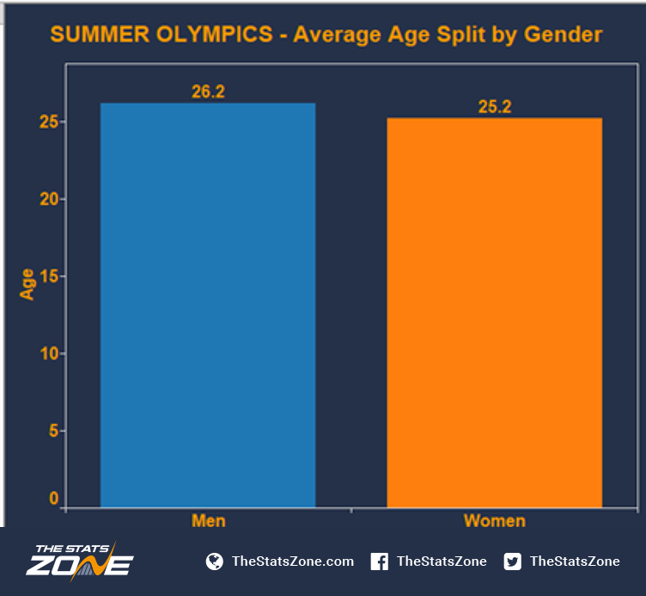
\includegraphics{age_olympics.png} \newline 
Source:
https://www.thestatszone.com/olympic-sports-how-does-peak-age-vary
\newline
\newline
NBA players are the elite athletes in their respective sports, so this
study shows that the reason MVP's are mostly around the age of 26-28 is
because an athlete reaches his prime at 26.2 years and starts to
gradually slow down.The following graph further shows the performance of
MLB players based on age groups. Although baseball is a different sport,
the concepts are all the same. All athletes in their respective field
experience the same prime years, and experience the same gradual
decrease in performance when they hit their 30s. \newline
\includegraphics{greatplayers.png} \newline  Source:
https://www.fangraphs.com/blogs/how-do-star-hitters-age/ \newline
\newline
What you can see from the chart above is that even hall of famers in
baseball could not maintain the same performance as they did whenthey
were in their mid to late 20s. This makes it clear that it is highly
unlikely for a player who is above the age of 30-32 years to become MVP.
SO therefore I conclude that any players above the age of 32 is highly
unlikelt to become mvp.

    \subsection{Kareem Abdul Jabbar career
analysis}\label{kareem-abdul-jabbar-career-analysis}

The further understand that players' performance slows down after the
age of 29, lets look at the MVP stats for Kareem Abdul Jabbar who is
leading the NBA with most MVP wins with \textbf{6}.

    \begin{Verbatim}[commandchars=\\\{\}]
{\color{incolor}In [{\color{incolor}605}]:} \PY{k}{def} \PY{n+nf}{getYear}\PY{p}{(}\PY{n}{year}\PY{p}{)}\PY{p}{:}
              \PY{k}{return} \PY{n}{year}\PY{p}{[}\PY{l+m+mi}{5}\PY{p}{:}\PY{p}{]}
          \PY{n}{years} \PY{o}{=} \PY{n}{getCsvData}\PY{p}{(}\PY{l+s+s1}{\PYZsq{}}\PY{l+s+s1}{mvp\PYZus{}1.csv}\PY{l+s+s1}{\PYZsq{}}\PY{p}{,}\PY{l+m+mi}{0}\PY{p}{,}\PY{l+s+s1}{\PYZsq{}}\PY{l+s+s1}{s}\PY{l+s+s1}{\PYZsq{}}\PY{p}{)}
          \PY{n}{mvp\PYZus{}name} \PY{o}{=} \PY{n}{getCsvData}\PY{p}{(}\PY{l+s+s1}{\PYZsq{}}\PY{l+s+s1}{mvp\PYZus{}1.csv}\PY{l+s+s1}{\PYZsq{}}\PY{p}{,}\PY{l+m+mi}{2}\PY{p}{,}\PY{l+s+s1}{\PYZsq{}}\PY{l+s+s1}{s}\PY{l+s+s1}{\PYZsq{}}\PY{p}{)}
          \PY{n}{minutes} \PY{o}{=} \PY{n}{getCsvData}\PY{p}{(}\PY{l+s+s1}{\PYZsq{}}\PY{l+s+s1}{mvp\PYZus{}1.csv}\PY{l+s+s1}{\PYZsq{}}\PY{p}{,}\PY{l+m+mi}{7}\PY{p}{,}\PY{l+s+s1}{\PYZsq{}}\PY{l+s+s1}{f}\PY{l+s+s1}{\PYZsq{}}\PY{p}{)}
          \PY{n}{points} \PY{o}{=} \PY{n}{getCsvData}\PY{p}{(}\PY{l+s+s1}{\PYZsq{}}\PY{l+s+s1}{mvp\PYZus{}1.csv}\PY{l+s+s1}{\PYZsq{}}\PY{p}{,}\PY{l+m+mi}{8}\PY{p}{,}\PY{l+s+s1}{\PYZsq{}}\PY{l+s+s1}{f}\PY{l+s+s1}{\PYZsq{}}\PY{p}{)}
          \PY{n}{rebounds} \PY{o}{=} \PY{n}{getCsvData}\PY{p}{(}\PY{l+s+s1}{\PYZsq{}}\PY{l+s+s1}{mvp\PYZus{}1.csv}\PY{l+s+s1}{\PYZsq{}}\PY{p}{,}\PY{l+m+mi}{9}\PY{p}{,}\PY{l+s+s1}{\PYZsq{}}\PY{l+s+s1}{f}\PY{l+s+s1}{\PYZsq{}}\PY{p}{)}
          \PY{n}{assists} \PY{o}{=} \PY{n}{getCsvData}\PY{p}{(}\PY{l+s+s1}{\PYZsq{}}\PY{l+s+s1}{mvp\PYZus{}1.csv}\PY{l+s+s1}{\PYZsq{}}\PY{p}{,}\PY{l+m+mi}{10}\PY{p}{,}\PY{l+s+s1}{\PYZsq{}}\PY{l+s+s1}{f}\PY{l+s+s1}{\PYZsq{}}\PY{p}{)}
          \PY{n}{win\PYZus{}shares} \PY{o}{=} \PY{n}{getCsvData}\PY{p}{(}\PY{l+s+s1}{\PYZsq{}}\PY{l+s+s1}{mvp\PYZus{}1.csv}\PY{l+s+s1}{\PYZsq{}}\PY{p}{,}\PY{l+m+mi}{15}\PY{p}{,}\PY{l+s+s1}{\PYZsq{}}\PY{l+s+s1}{f}\PY{l+s+s1}{\PYZsq{}}\PY{p}{)}
          \PY{n}{kareem\PYZus{}years} \PY{o}{=} \PY{p}{[}\PY{p}{]}
          \PY{n}{kareem\PYZus{}min} \PY{o}{=} \PY{p}{[}\PY{p}{]}
          \PY{n}{kareem\PYZus{}points} \PY{o}{=} \PY{p}{[}\PY{p}{]}
          \PY{n}{kareem\PYZus{}reb} \PY{o}{=} \PY{p}{[}\PY{p}{]}
          \PY{n}{kareem\PYZus{}ass} \PY{o}{=} \PY{p}{[}\PY{p}{]}
          \PY{n}{kareem\PYZus{}win} \PY{o}{=} \PY{p}{[}\PY{p}{]}
          \PY{n}{index} \PY{o}{=} \PY{l+m+mi}{0}
          \PY{n}{kareem\PYZus{}index} \PY{o}{=} \PY{p}{[}\PY{p}{]}
          \PY{k}{for} \PY{n}{i} \PY{o+ow}{in} \PY{n}{mvp\PYZus{}name}\PY{p}{:}
              \PY{k}{if}\PY{p}{(}\PY{n}{i} \PY{o}{==} \PY{l+s+s1}{\PYZsq{}}\PY{l+s+s1}{Kareem Abdul\PYZhy{}Jabbar}\PY{l+s+s1}{\PYZsq{}}\PY{p}{)}\PY{p}{:}
                  \PY{n}{kareem\PYZus{}index}\PY{o}{.}\PY{n}{append}\PY{p}{(}\PY{n}{index}\PY{p}{)}
              \PY{n}{index}\PY{o}{+}\PY{o}{=}\PY{l+m+mi}{1}
          \PY{k}{for} \PY{n}{i} \PY{o+ow}{in} \PY{n+nb}{reversed}\PY{p}{(}\PY{n+nb}{range}\PY{p}{(}\PY{n+nb}{len}\PY{p}{(}\PY{n}{kareem\PYZus{}index}\PY{p}{)}\PY{p}{)}\PY{p}{)}\PY{p}{:}
              \PY{n}{kareem\PYZus{}years}\PY{o}{.}\PY{n}{append}\PY{p}{(}\PY{n}{getYear}\PY{p}{(}\PY{n}{years}\PY{p}{[}\PY{n}{kareem\PYZus{}index}\PY{p}{[}\PY{n}{i}\PY{p}{]}\PY{p}{]}\PY{p}{)}\PY{p}{)}
              \PY{n}{kareem\PYZus{}min}\PY{o}{.}\PY{n}{append}\PY{p}{(}\PY{n}{minutes}\PY{p}{[}\PY{n}{kareem\PYZus{}index}\PY{p}{[}\PY{n}{i}\PY{p}{]}\PY{p}{]}\PY{p}{)}
              \PY{n}{kareem\PYZus{}points}\PY{o}{.}\PY{n}{append}\PY{p}{(}\PY{n}{points}\PY{p}{[}\PY{n}{kareem\PYZus{}index}\PY{p}{[}\PY{n}{i}\PY{p}{]}\PY{p}{]}\PY{p}{)}
              \PY{n}{kareem\PYZus{}reb}\PY{o}{.}\PY{n}{append}\PY{p}{(}\PY{n}{rebounds}\PY{p}{[}\PY{n}{kareem\PYZus{}index}\PY{p}{[}\PY{n}{i}\PY{p}{]}\PY{p}{]}\PY{p}{)}
              \PY{n}{kareem\PYZus{}ass}\PY{o}{.}\PY{n}{append}\PY{p}{(}\PY{n}{assists}\PY{p}{[}\PY{n}{kareem\PYZus{}index}\PY{p}{[}\PY{n}{i}\PY{p}{]}\PY{p}{]}\PY{p}{)}
              \PY{n}{kareem\PYZus{}win}\PY{o}{.}\PY{n}{append}\PY{p}{(}\PY{n}{win\PYZus{}shares}\PY{p}{[}\PY{n}{kareem\PYZus{}index}\PY{p}{[}\PY{n}{i}\PY{p}{]}\PY{p}{]}\PY{p}{)}   
          \PY{n}{plt}\PY{o}{.}\PY{n}{plot}\PY{p}{(}\PY{p}{[}\PY{p}{]}\PY{p}{,}\PY{p}{[}\PY{p}{]}\PY{p}{,}\PY{n}{color}\PY{o}{=}\PY{l+s+s1}{\PYZsq{}}\PY{l+s+s1}{m}\PY{l+s+s1}{\PYZsq{}}\PY{p}{,}\PY{n}{label}\PY{o}{=}\PY{l+s+s1}{\PYZsq{}}\PY{l+s+s1}{Minutes}\PY{l+s+s1}{\PYZsq{}}\PY{p}{,}\PY{n}{linewidth}\PY{o}{=}\PY{l+m+mi}{5}\PY{p}{)}
          \PY{n}{plt}\PY{o}{.}\PY{n}{plot}\PY{p}{(}\PY{p}{[}\PY{p}{]}\PY{p}{,}\PY{p}{[}\PY{p}{]}\PY{p}{,}\PY{n}{color}\PY{o}{=}\PY{l+s+s1}{\PYZsq{}}\PY{l+s+s1}{c}\PY{l+s+s1}{\PYZsq{}}\PY{p}{,}\PY{n}{label}\PY{o}{=}\PY{l+s+s1}{\PYZsq{}}\PY{l+s+s1}{Points}\PY{l+s+s1}{\PYZsq{}}\PY{p}{,}\PY{n}{linewidth}\PY{o}{=}\PY{l+m+mi}{5}\PY{p}{)}
          \PY{n}{plt}\PY{o}{.}\PY{n}{plot}\PY{p}{(}\PY{p}{[}\PY{p}{]}\PY{p}{,}\PY{p}{[}\PY{p}{]}\PY{p}{,}\PY{n}{color}\PY{o}{=}\PY{l+s+s1}{\PYZsq{}}\PY{l+s+s1}{r}\PY{l+s+s1}{\PYZsq{}}\PY{p}{,}\PY{n}{label}\PY{o}{=}\PY{l+s+s1}{\PYZsq{}}\PY{l+s+s1}{Rebounds}\PY{l+s+s1}{\PYZsq{}}\PY{p}{,}\PY{n}{linewidth}\PY{o}{=}\PY{l+m+mi}{5}\PY{p}{)}
          \PY{n}{plt}\PY{o}{.}\PY{n}{plot}\PY{p}{(}\PY{p}{[}\PY{p}{]}\PY{p}{,}\PY{p}{[}\PY{p}{]}\PY{p}{,}\PY{n}{color}\PY{o}{=}\PY{l+s+s1}{\PYZsq{}}\PY{l+s+s1}{b}\PY{l+s+s1}{\PYZsq{}}\PY{p}{,}\PY{n}{label}\PY{o}{=}\PY{l+s+s1}{\PYZsq{}}\PY{l+s+s1}{Assists}\PY{l+s+s1}{\PYZsq{}}\PY{p}{,}\PY{n}{linewidth}\PY{o}{=}\PY{l+m+mi}{5}\PY{p}{)}
          \PY{n}{plt}\PY{o}{.}\PY{n}{plot}\PY{p}{(}\PY{p}{[}\PY{p}{]}\PY{p}{,}\PY{p}{[}\PY{p}{]}\PY{p}{,}\PY{n}{color}\PY{o}{=}\PY{l+s+s1}{\PYZsq{}}\PY{l+s+s1}{k}\PY{l+s+s1}{\PYZsq{}}\PY{p}{,}\PY{n}{label}\PY{o}{=}\PY{l+s+s1}{\PYZsq{}}\PY{l+s+s1}{Win Shares}\PY{l+s+s1}{\PYZsq{}}\PY{p}{,}\PY{n}{linewidth}\PY{o}{=}\PY{l+m+mi}{5}\PY{p}{)}
          \PY{n}{plt}\PY{o}{.}\PY{n}{stackplot}\PY{p}{(}\PY{n}{kareem\PYZus{}years}\PY{p}{,}\PY{n}{kareem\PYZus{}min}\PY{p}{,}\PY{n}{kareem\PYZus{}points}\PY{p}{,}\PY{n}{kareem\PYZus{}reb}\PY{p}{,}\PY{n}{kareem\PYZus{}ass}\PY{p}{,}\PY{n}{kareem\PYZus{}win}\PY{p}{,}\PY{n}{colors}\PY{o}{=}\PY{p}{[}\PY{l+s+s1}{\PYZsq{}}\PY{l+s+s1}{m}\PY{l+s+s1}{\PYZsq{}}\PY{p}{,}\PY{l+s+s1}{\PYZsq{}}\PY{l+s+s1}{c}\PY{l+s+s1}{\PYZsq{}}\PY{p}{,}\PY{l+s+s1}{\PYZsq{}}\PY{l+s+s1}{r}\PY{l+s+s1}{\PYZsq{}}\PY{p}{,}\PY{l+s+s1}{\PYZsq{}}\PY{l+s+s1}{b}\PY{l+s+s1}{\PYZsq{}}\PY{p}{,}\PY{l+s+s1}{\PYZsq{}}\PY{l+s+s1}{k}\PY{l+s+s1}{\PYZsq{}}\PY{p}{,}\PY{l+s+s1}{\PYZsq{}}\PY{l+s+s1}{g}\PY{l+s+s1}{\PYZsq{}}\PY{p}{]}\PY{p}{)}
          \PY{n}{plt}\PY{o}{.}\PY{n}{xlabel}\PY{p}{(}\PY{l+s+s1}{\PYZsq{}}\PY{l+s+s1}{Year}\PY{l+s+s1}{\PYZsq{}}\PY{p}{)}
          \PY{n}{plt}\PY{o}{.}\PY{n}{ylabel}\PY{p}{(}\PY{l+s+s1}{\PYZsq{}}\PY{l+s+s1}{Y}\PY{l+s+s1}{\PYZsq{}}\PY{p}{)}
          \PY{n}{plt}\PY{o}{.}\PY{n}{title}\PY{p}{(}\PY{l+s+s1}{\PYZsq{}}\PY{l+s+s1}{Kareem Abdul Jabbar Career Stack Plot}\PY{l+s+s1}{\PYZsq{}}\PY{p}{)}
          \PY{n}{plt}\PY{o}{.}\PY{n}{legend}\PY{p}{(}\PY{p}{)}
          \PY{n}{plt}\PY{o}{.}\PY{n}{show}\PY{p}{(}\PY{p}{)}
\end{Verbatim}


    \begin{center}
    \adjustimage{max size={0.9\linewidth}{0.9\paperheight}}{output_53_0.png}
    \end{center}
    { \hspace*{\fill} \\}
    
    \textbf{Analysis} \newline

As shown in the stack plot above, we can see that Kareem Abdul Jabbar's
performance slowed down each year in every aspect. He still managed to
be crowned MVP but his last MVP ring which was awarded at the age of 32
did not siginify his best career performance. This graph is a perfect
representation of why MVP's are mostly in the range of 26-29 years og
age and struggle to become MVP after that.

\subsection{MVP Demographics}\label{mvp-demographics}

Let us now look at the demographics of the MVP's by State

    \begin{Verbatim}[commandchars=\\\{\}]
{\color{incolor}In [{\color{incolor}606}]:} \PY{n}{born} \PY{o}{=} \PY{n}{getCsvData}\PY{p}{(}\PY{l+s+s1}{\PYZsq{}}\PY{l+s+s1}{mvp\PYZus{}1.csv}\PY{l+s+s1}{\PYZsq{}}\PY{p}{,}\PY{l+m+mi}{19}\PY{p}{,}\PY{l+s+s1}{\PYZsq{}}\PY{l+s+s1}{s}\PY{l+s+s1}{\PYZsq{}}\PY{p}{)}
          \PY{n}{name} \PY{o}{=} \PY{n}{getCsvData}\PY{p}{(}\PY{l+s+s1}{\PYZsq{}}\PY{l+s+s1}{mvp\PYZus{}1.csv}\PY{l+s+s1}{\PYZsq{}}\PY{p}{,}\PY{l+m+mi}{2}\PY{p}{,} \PY{l+s+s1}{\PYZsq{}}\PY{l+s+s1}{s}\PY{l+s+s1}{\PYZsq{}}\PY{p}{)}
          \PY{n}{index} \PY{o}{=} \PY{l+m+mi}{0}
          \PY{n}{born\PYZus{}dic} \PY{o}{=} \PY{p}{\PYZob{}}\PY{p}{\PYZcb{}}
          \PY{n}{states} \PY{o}{=} \PY{p}{[}\PY{p}{]}
          \PY{n}{names} \PY{o}{=} \PY{p}{[}\PY{p}{]}
          \PY{n}{state\PYZus{}names} \PY{o}{=} \PY{p}{[}\PY{p}{]}
          \PY{k}{for} \PY{n}{i} \PY{o+ow}{in} \PY{n}{born}\PY{p}{:}
              \PY{n}{born\PYZus{}dic}\PY{p}{[}\PY{n}{name}\PY{p}{[}\PY{n}{index}\PY{p}{]}\PY{p}{]} \PY{o}{=} \PY{n}{i}
              \PY{n}{index}\PY{o}{+}\PY{o}{=}\PY{l+m+mi}{1}
          \PY{k}{for} \PY{n}{key} \PY{o+ow}{in} \PY{n}{born\PYZus{}dic}\PY{p}{:}
              \PY{n}{states}\PY{o}{.}\PY{n}{append}\PY{p}{(}\PY{n}{born\PYZus{}dic}\PY{p}{[}\PY{n}{key}\PY{p}{]}\PY{p}{)}
          \PY{n}{state\PYZus{}count} \PY{o}{=} \PY{n}{Counter}\PY{p}{(}\PY{n}{states}\PY{p}{)}
          \PY{n}{ind} \PY{o}{=} \PY{l+m+mi}{0}
          \PY{k}{for} \PY{n}{key} \PY{o+ow}{in} \PY{n}{state\PYZus{}count}\PY{p}{:}
              \PY{n}{state\PYZus{}names}\PY{o}{.}\PY{n}{append}\PY{p}{(}\PY{n}{key}\PY{p}{)}
              \PY{n}{names}\PY{o}{.}\PY{n}{append}\PY{p}{(}\PY{n}{state\PYZus{}count}\PY{p}{[}\PY{n}{key}\PY{p}{]}\PY{p}{)}
          \PY{n}{plt}\PY{o}{.}\PY{n}{pie}\PY{p}{(}\PY{n}{names}\PY{p}{,}
              \PY{n}{labels}\PY{o}{=}\PY{n}{state\PYZus{}names}\PY{p}{,}
              \PY{n}{startangle} \PY{o}{=} \PY{l+m+mi}{90}\PY{p}{,}
              \PY{n}{shadow} \PY{o}{=} \PY{k+kc}{True}\PY{p}{,}
              \PY{n}{autopct}\PY{o}{=}\PY{l+s+s1}{\PYZsq{}}\PY{l+s+si}{\PYZpc{}1.1f}\PY{l+s+si}{\PYZpc{}\PYZpc{}}\PY{l+s+s1}{\PYZsq{}}\PY{p}{)}
          \PY{n}{plt}\PY{o}{.}\PY{n}{title}\PY{p}{(}\PY{l+s+s1}{\PYZsq{}}\PY{l+s+s1}{Demographics}\PY{l+s+s1}{\PYZsq{}}\PY{p}{)}
          \PY{n}{plt}\PY{o}{.}\PY{n}{show}\PY{p}{(}\PY{p}{)}
\end{Verbatim}


    \begin{center}
    \adjustimage{max size={0.9\linewidth}{0.9\paperheight}}{output_55_0.png}
    \end{center}
    { \hspace*{\fill} \\}
    
    \textbf{Analysis} \newline

From the pie chart, 25\% of MVP's come from only 2 states! There have
been MVP's from 21 different places around the world, but interestingly,
1/4 come from either New York or Louisiana. Basketball is one of the
most popular sports in the world, and to know that only 2 states account
for 25\% of MVP's in the last 62 years is quite interesting. The
question is what is so special about these two states that produce 25\%
of the MVP's from the last 6 to 7 decades? \newline
\newline
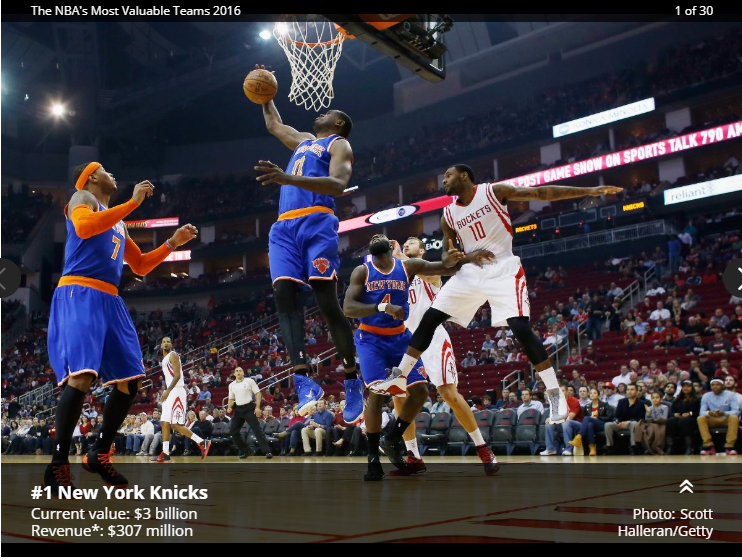
\includegraphics{nykworth1.png} \newline  Source:
https://www.forbes.com/pictures/mli45fflmj/1-new-york-knicks/\#3382942f2de0
\newline
\newline
In study done by Forbes.com in 2016, the New York Knicks are ranked 1 as
the most valuable team in the NBA. Their networth is \textbf{3 billion}
dollars and they rack in \textbf{300 million dollars} of revenue each
year! The reason this is important is because this shows how popular
basketball is in New York \newline
\newline
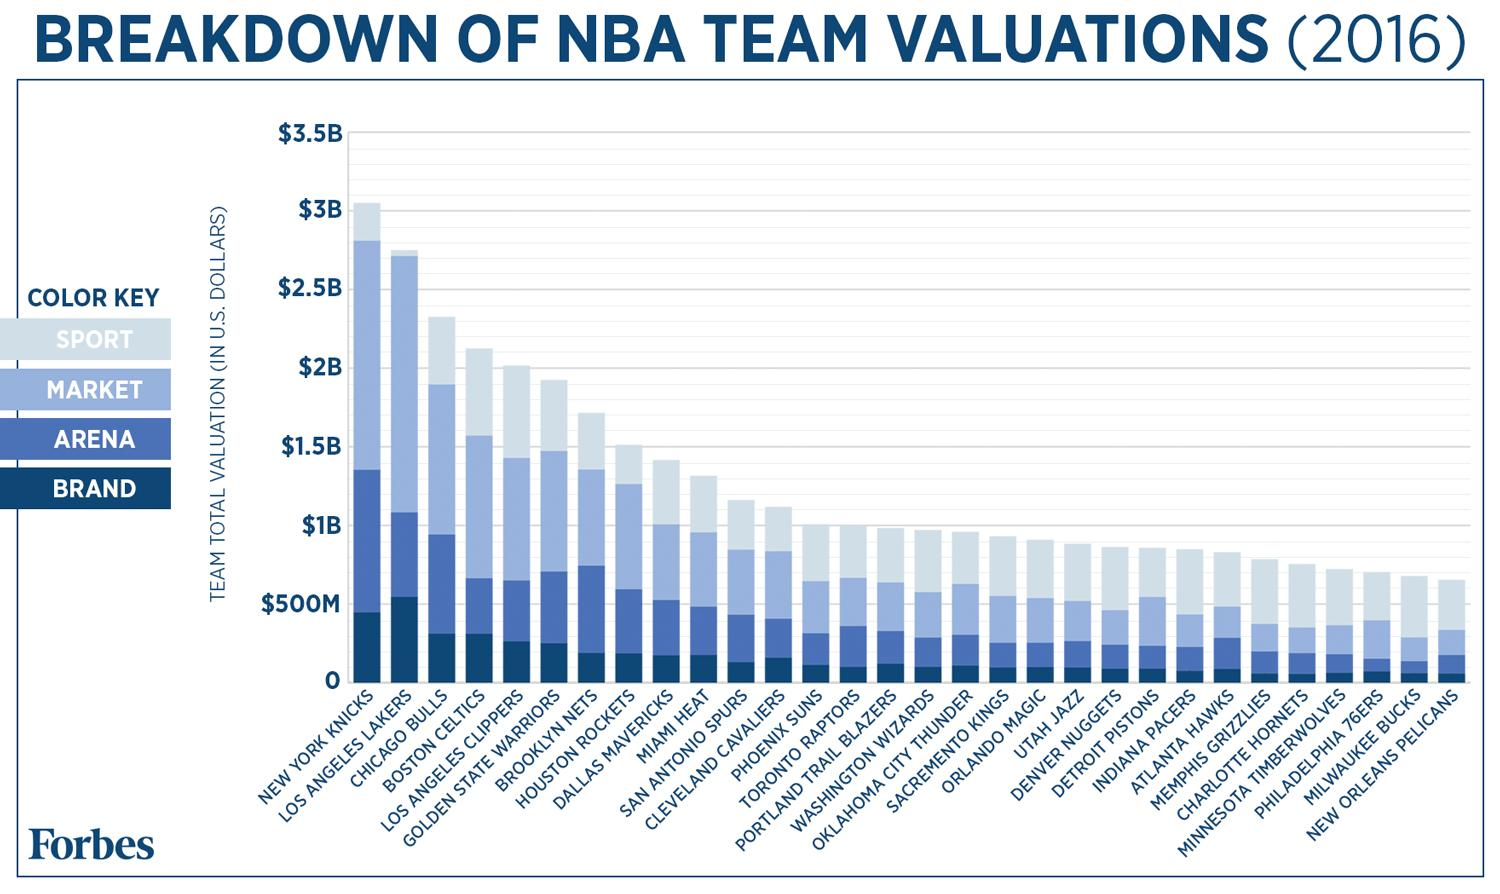
\includegraphics{knicks_income.png} \newline
Source:
https://www.forbes.com/sites/baileybrautigan/2016/03/21/where-all-that-money-comes-from-nba-team-valuations-visualized/\#3733bd89444f
\newline
\newline
The New York Knicks large dominance over the market share shows the
popularity of basketball in New York. This will in turn motivate and
produce great players.In addition, according to bleachreport.com, the
state of New York is \textbf{ranked number 3} in producing the best high
school players. Also, in a study conducted in 2010, New York was
\textbf{ranked third} by Gross Domestic Product with a \textbf{GDP of
1.2 Trillion dollars!} New York accounts for 8.1 percent of the total
GDP in the United States. The below picture gives a nice visualization
of how large New York's economy is in comparison to other states.
\newline  \newline
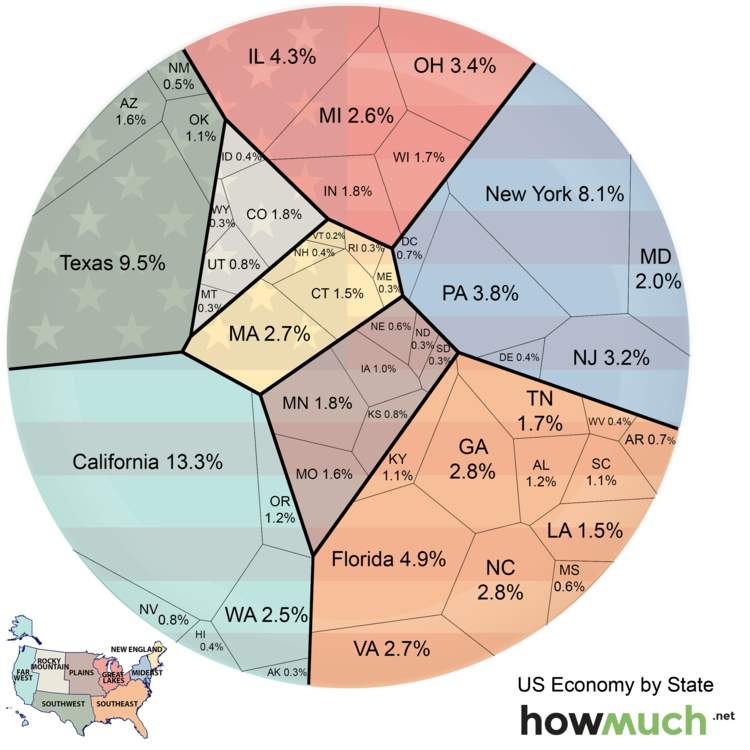
\includegraphics{ny_gdp.png} \newline  Source:
http://www.businessinsider.com/how-much-each-state-contributes-to-the-us-economy-2015-9
\newline
\newline
Lasty, New York ranks \textbf{third} in incomer per two-bedroom housing.
This further explaines that New York has more income for most household,
who then could provide more opportunities and resources for kids to
excel in athletics. \newline
\newline
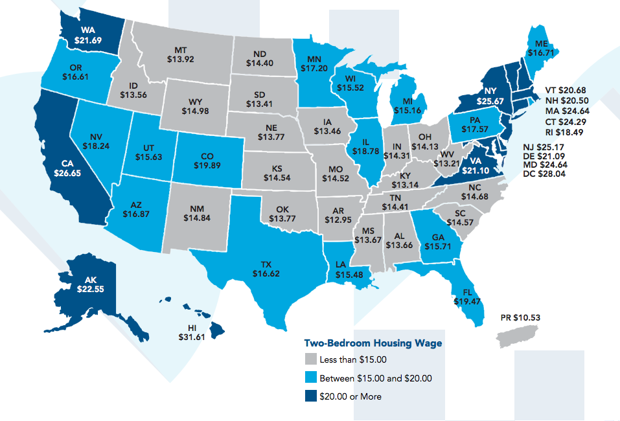
\includegraphics{newyork_income.png} \newline  Source:
https://www.citylab.com/equity/2015/05/mapping-the-hourly-wage-needed-to-rent-a-2-bedroom-apartment-in-every-us-state/394142/
\newline
\newline
Lousiniana does not compare to New York in GDP, but it is \textbf{ranked
5} by bleachreport in 2017 as producing some of the most talented
athletes. This is definitly a factor as to why Louisiana has had so many
MVP's. 

    \subsection{MVP Positions}\label{mvp-positions}

Lets look at the distribution of NBA positions

    \begin{Verbatim}[commandchars=\\\{\}]
{\color{incolor}In [{\color{incolor}607}]:} \PY{k}{def} \PY{n+nf}{posReduce}\PY{p}{(}\PY{n}{pos}\PY{p}{)}\PY{p}{:}
              \PY{n}{lis} \PY{o}{=} \PY{p}{[}\PY{l+m+mi}{0}\PY{p}{]}\PY{o}{*}\PY{l+m+mi}{5}
              \PY{k}{for} \PY{n}{i} \PY{o+ow}{in} \PY{n}{pos}\PY{p}{:}
                  \PY{k}{if}\PY{p}{(}\PY{n}{i}\PY{o}{==}\PY{l+s+s1}{\PYZsq{}}\PY{l+s+s1}{PointGuard}\PY{l+s+s1}{\PYZsq{}}\PY{p}{)}\PY{p}{:}
                      \PY{n}{lis}\PY{p}{[}\PY{l+m+mi}{0}\PY{p}{]}\PY{o}{+}\PY{o}{=}\PY{l+m+mi}{1}
                  \PY{k}{elif}\PY{p}{(}\PY{n}{i}\PY{o}{==}\PY{l+s+s1}{\PYZsq{}}\PY{l+s+s1}{ShootingGuard}\PY{l+s+s1}{\PYZsq{}}\PY{p}{)}\PY{p}{:}
                      \PY{n}{lis}\PY{p}{[}\PY{l+m+mi}{1}\PY{p}{]}\PY{o}{+}\PY{o}{=}\PY{l+m+mi}{1}
                  \PY{k}{elif}\PY{p}{(}\PY{n}{i}\PY{o}{==}\PY{l+s+s1}{\PYZsq{}}\PY{l+s+s1}{SmallForward}\PY{l+s+s1}{\PYZsq{}}\PY{p}{)}\PY{p}{:}
                      \PY{n}{lis}\PY{p}{[}\PY{l+m+mi}{2}\PY{p}{]}\PY{o}{+}\PY{o}{=}\PY{l+m+mi}{1}
                  \PY{k}{elif}\PY{p}{(}\PY{n}{i}\PY{o}{==}\PY{l+s+s1}{\PYZsq{}}\PY{l+s+s1}{PowerForward}\PY{l+s+s1}{\PYZsq{}}\PY{p}{)}\PY{p}{:}
                      \PY{n}{lis}\PY{p}{[}\PY{l+m+mi}{3}\PY{p}{]}\PY{o}{+}\PY{o}{=}\PY{l+m+mi}{1}
                  \PY{k}{else}\PY{p}{:}
                      \PY{n}{lis}\PY{p}{[}\PY{l+m+mi}{4}\PY{p}{]}\PY{o}{+}\PY{o}{=}\PY{l+m+mi}{1}
              \PY{k}{return} \PY{n}{lis}
          \PY{n}{position} \PY{o}{=} \PY{n}{getCsvData}\PY{p}{(}\PY{l+s+s1}{\PYZsq{}}\PY{l+s+s1}{mvp\PYZus{}1.csv}\PY{l+s+s1}{\PYZsq{}}\PY{p}{,}\PY{l+m+mi}{18}\PY{p}{,}\PY{l+s+s1}{\PYZsq{}}\PY{l+s+s1}{s}\PY{l+s+s1}{\PYZsq{}}\PY{p}{)}
          \PY{n}{real\PYZus{}position} \PY{o}{=} \PY{p}{[}\PY{p}{]}
          \PY{k}{for} \PY{n}{i} \PY{o+ow}{in} \PY{n}{position}\PY{p}{:}
              \PY{n}{lis} \PY{o}{=} \PY{n}{i}\PY{o}{.}\PY{n}{split}\PY{p}{(}\PY{l+s+s1}{\PYZsq{}}\PY{l+s+s1}{and}\PY{l+s+s1}{\PYZsq{}}\PY{p}{)}
              \PY{n}{real\PYZus{}position}\PY{o}{.}\PY{n}{append}\PY{p}{(}\PY{n}{lis}\PY{p}{[}\PY{o}{\PYZhy{}}\PY{l+m+mi}{1}\PY{p}{]}\PY{p}{)}
          \PY{n}{pos\PYZus{}list} \PY{o}{=} \PY{n}{posReduce}\PY{p}{(}\PY{n}{real\PYZus{}position}\PY{p}{)}
          \PY{n}{plt}\PY{o}{.}\PY{n}{style}\PY{o}{.}\PY{n}{use}\PY{p}{(}\PY{l+s+s1}{\PYZsq{}}\PY{l+s+s1}{ggplot}\PY{l+s+s1}{\PYZsq{}}\PY{p}{)}
          \PY{n}{pos} \PY{o}{=} \PY{p}{[}\PY{l+s+s1}{\PYZsq{}}\PY{l+s+s1}{PG}\PY{l+s+s1}{\PYZsq{}}\PY{p}{,} \PY{l+s+s1}{\PYZsq{}}\PY{l+s+s1}{SG}\PY{l+s+s1}{\PYZsq{}}\PY{p}{,} \PY{l+s+s1}{\PYZsq{}}\PY{l+s+s1}{SF}\PY{l+s+s1}{\PYZsq{}}\PY{p}{,} \PY{l+s+s1}{\PYZsq{}}\PY{l+s+s1}{PF}\PY{l+s+s1}{\PYZsq{}}\PY{p}{,} \PY{l+s+s1}{\PYZsq{}}\PY{l+s+s1}{C}\PY{l+s+s1}{\PYZsq{}}\PY{p}{]}
          \PY{n}{plt}\PY{o}{.}\PY{n}{bar}\PY{p}{(}\PY{n}{pos}\PY{p}{,} \PY{n}{pos\PYZus{}list}\PY{p}{,} \PY{n}{color}\PY{o}{=}\PY{l+s+s1}{\PYZsq{}}\PY{l+s+s1}{green}\PY{l+s+s1}{\PYZsq{}}\PY{p}{)}
          \PY{n}{plt}\PY{o}{.}\PY{n}{xlabel}\PY{p}{(}\PY{l+s+s2}{\PYZdq{}}\PY{l+s+s2}{Position}\PY{l+s+s2}{\PYZdq{}}\PY{p}{)}
          \PY{n}{plt}\PY{o}{.}\PY{n}{ylabel}\PY{p}{(}\PY{l+s+s2}{\PYZdq{}}\PY{l+s+s2}{Amount}\PY{l+s+s2}{\PYZdq{}}\PY{p}{)}
          \PY{n}{plt}\PY{o}{.}\PY{n}{title}\PY{p}{(}\PY{l+s+s2}{\PYZdq{}}\PY{l+s+s2}{Positions}\PY{l+s+s2}{\PYZdq{}}\PY{p}{)}
          \PY{n}{plt}\PY{o}{.}\PY{n}{show}\PY{p}{(}\PY{p}{)}
          \PY{n}{x} \PY{o}{=} \PY{p}{(}\PY{n}{pos\PYZus{}list}\PY{p}{[}\PY{l+m+mi}{4}\PY{p}{]} \PY{o}{+} \PY{n}{pos\PYZus{}list}\PY{p}{[}\PY{l+m+mi}{3}\PY{p}{]}\PY{p}{)}\PY{o}{/}\PY{l+m+mi}{62}
          \PY{n}{years} \PY{o}{=} \PY{p}{[}\PY{p}{]}
          \PY{n}{big\PYZus{}men} \PY{o}{=} \PY{p}{[}\PY{p}{]}
          \PY{n}{y} \PY{o}{=} \PY{n}{getCsvData}\PY{p}{(}\PY{l+s+s1}{\PYZsq{}}\PY{l+s+s1}{mvp\PYZus{}1.csv}\PY{l+s+s1}{\PYZsq{}}\PY{p}{,}\PY{l+m+mi}{0}\PY{p}{,}\PY{l+s+s1}{\PYZsq{}}\PY{l+s+s1}{s}\PY{l+s+s1}{\PYZsq{}}\PY{p}{)}
          \PY{k}{for} \PY{n}{i} \PY{o+ow}{in} \PY{n+nb}{reversed}\PY{p}{(}\PY{n+nb}{range}\PY{p}{(}\PY{n+nb}{len}\PY{p}{(}\PY{n}{y}\PY{p}{)}\PY{p}{)}\PY{p}{)}\PY{p}{:}
              \PY{n}{years}\PY{o}{.}\PY{n}{append}\PY{p}{(}\PY{n}{getYear}\PY{p}{(}\PY{n}{y}\PY{p}{[}\PY{n}{i}\PY{p}{]}\PY{p}{)}\PY{p}{)}
              \PY{n}{lis} \PY{o}{=} \PY{n}{position}\PY{p}{[}\PY{n}{i}\PY{p}{]}\PY{o}{.}\PY{n}{split}\PY{p}{(}\PY{l+s+s1}{\PYZsq{}}\PY{l+s+s1}{and}\PY{l+s+s1}{\PYZsq{}}\PY{p}{)}
              \PY{k}{if}\PY{p}{(}\PY{l+s+s1}{\PYZsq{}}\PY{l+s+s1}{PowerForward}\PY{l+s+s1}{\PYZsq{}} \PY{o+ow}{in} \PY{n}{lis} \PY{o+ow}{or} \PY{l+s+s1}{\PYZsq{}}\PY{l+s+s1}{Center}\PY{l+s+s1}{\PYZsq{}} \PY{o+ow}{in} \PY{n}{lis}\PY{p}{)}\PY{p}{:}
                  \PY{n}{big\PYZus{}men}\PY{o}{.}\PY{n}{append}\PY{p}{(}\PY{l+m+mi}{1}\PY{p}{)}
\end{Verbatim}


    \begin{center}
    \adjustimage{max size={0.9\linewidth}{0.9\paperheight}}{output_58_0.png}
    \end{center}
    { \hspace*{\fill} \\}
    
    \textbf{Analysis} \newline

This bar graph shows that 63 percent of the MVP's from the last 60 years
were big men. Furthermore, the first \textbf{30 years} of MVPS from
\textbf{1955-1985} were all Big men! The question is why were big men
soo dominant, especially from the years 1955-1985? The following gif
illustrates some good insight as to why this was the case
\textbf{Please} open the link to the Gif link below, that illustrates
the height changes over the years. \newline
Source:
http://www.tothemean.com/images/2014.08.27.viraj/seasons.height-75c9c0d1.gif
\newline
After examining the Gif link from above, from 1955-1985, most of the
players were smaller guys, and there were hardly any big men at the
time. So how does this explain the large percentage of big men as MVP's?
Well for one, less big men means there are less big men that are
defending and giving trouble to big men that were playing at the time.
Second, there was larger percentage of smaller players, so these smaller
players were easily dominated by the big men. This gave big men an open
floor to dominate over the smaller players-\/-very much like the David
and Goliath type scenario. Furthermore, during the mid 1980's a larger
distribution of big men started playing in the NBA which then made it
harder to succeed as a big since there was more competition. 

    \section{Machine Learning}\label{machine-learning}

    \subsubsection{Prediction}\label{prediction}

There were many considerations as to what would the main focus of my
prediction. The orginal plan was to predict the MVP but sadly there was
not a large enough data set for this task.

    \textbf{Challenge}

\begin{itemize}
\tightlist
\item
  62 years of MVP's did not produce enough rows or data to make a proper
  Machine Learning model. \newline
\end{itemize}

\textbf{Opportunity}

\begin{itemize}
\item
  When I was scraping my data from Basketball-reference.com. One set of
  data that I scraped was the voting stastics for each years MVP. This
  data set consists of the top 10 to 15 players who were considered in
  the race for the MVP spot. Each player from the voting list for each
  year was given a certain amount of voting points based on their
  performance. Features such as Points per game, Assists per game, and
  Rebounds per game has a hefty influence on the amount of voting points
  a player received. After receiving voting points, a player is then
  ranked from best to worst.
\item
  For each year, the players were given a rank from lets say 1-10 where
  the 1st ranked player earned the most points and was awarded the MVP
  crown. The second ranked player was a close second and so on.
\end{itemize}

\textbf{Decision} \newline

\begin{itemize}
\tightlist
\item
  I decided to look at this voting data set for my Machine Learning
  portion of this project. With more or less 60 years of MVP's and 10 to
  15 players in the voting list per year gave me approximately 960 rows
  of data.
\end{itemize}

    \subsection{Features that matter:}\label{features-that-matter}

In my attempt to search for the best features for my Machine learning
Models, I plotted some features to see which ones had a good coreleation
between a players rank and the feature. So for Points per game, I wanted
to see if the higher ranked player you are, will that mean you will
score more points. I did this for many features and this was my finding.

    \begin{Verbatim}[commandchars=\\\{\}]
{\color{incolor}In [{\color{incolor}608}]:} \PY{k+kn}{import} \PY{n+nn}{pandas} \PY{k}{as} \PY{n+nn}{pd}
          \PY{k+kn}{import} \PY{n+nn}{numpy} \PY{k}{as} \PY{n+nn}{np}
          \PY{k+kn}{import} \PY{n+nn}{pandas\PYZus{}ml} \PY{k}{as} \PY{n+nn}{pdml}
          \PY{k+kn}{import} \PY{n+nn}{sklearn}\PY{n+nn}{.}\PY{n+nn}{datasets}
          \PY{k+kn}{import} \PY{n+nn}{seaborn} \PY{k}{as} \PY{n+nn}{sns}
          
          \PY{n}{voting} \PY{o}{=} \PY{n}{pd}\PY{o}{.}\PY{n}{read\PYZus{}csv}\PY{p}{(}\PY{l+s+s1}{\PYZsq{}}\PY{l+s+s1}{voting\PYZus{}mvp.csv}\PY{l+s+s1}{\PYZsq{}}\PY{p}{,}\PY{n}{usecols}\PY{o}{=}\PY{p}{[}\PY{l+m+mi}{0}\PY{p}{,}\PY{l+m+mi}{10}\PY{p}{,}\PY{l+m+mi}{11}\PY{p}{,}\PY{l+m+mi}{12}\PY{p}{,}\PY{l+m+mi}{18}\PY{p}{]}\PY{p}{)}
          \PY{n}{d} \PY{o}{=} \PY{n}{pd}\PY{o}{.}\PY{n}{read\PYZus{}csv}\PY{p}{(}\PY{l+s+s1}{\PYZsq{}}\PY{l+s+s1}{voting\PYZus{}mvp.csv}\PY{l+s+s1}{\PYZsq{}}\PY{p}{,}\PY{n}{usecols}\PY{o}{=}\PY{p}{[}\PY{l+m+mi}{10}\PY{p}{,}\PY{l+m+mi}{11}\PY{p}{,}\PY{l+m+mi}{12}\PY{p}{,}\PY{l+m+mi}{18}\PY{p}{]}\PY{p}{)}
          \PY{n}{target} \PY{o}{=} \PY{p}{[}\PY{p}{]}
          \PY{k}{for} \PY{n}{index}\PY{p}{,} \PY{n}{row} \PY{o+ow}{in} \PY{n}{voting}\PY{o}{.}\PY{n}{iterrows}\PY{p}{(}\PY{p}{)}\PY{p}{:}
              \PY{k}{if}\PY{p}{(}\PY{n}{row}\PY{p}{[}\PY{l+s+s1}{\PYZsq{}}\PY{l+s+s1}{Rank}\PY{l+s+s1}{\PYZsq{}}\PY{p}{]}\PY{o}{\PYZlt{}}\PY{o}{=}\PY{l+m+mi}{3}\PY{p}{)}\PY{p}{:}
                  \PY{n}{target}\PY{o}{.}\PY{n}{append}\PY{p}{(}\PY{l+m+mi}{0}\PY{p}{)}
              \PY{k}{elif}\PY{p}{(}\PY{n}{row}\PY{p}{[}\PY{l+s+s1}{\PYZsq{}}\PY{l+s+s1}{Rank}\PY{l+s+s1}{\PYZsq{}}\PY{p}{]}\PY{o}{\PYZgt{}}\PY{l+m+mi}{3} \PY{o+ow}{and} \PY{n}{row}\PY{p}{[}\PY{l+s+s1}{\PYZsq{}}\PY{l+s+s1}{Rank}\PY{l+s+s1}{\PYZsq{}}\PY{p}{]}\PY{o}{\PYZlt{}}\PY{o}{=}\PY{l+m+mi}{7}\PY{p}{)}\PY{p}{:}
                  \PY{n}{target}\PY{o}{.}\PY{n}{append}\PY{p}{(}\PY{l+m+mi}{1}\PY{p}{)}
              \PY{k}{else}\PY{p}{:}
                  \PY{n}{target}\PY{o}{.}\PY{n}{append}\PY{p}{(}\PY{l+m+mi}{2}\PY{p}{)}
          \PY{n}{final\PYZus{}df} \PY{o}{=} \PY{n}{d}\PY{o}{.}\PY{n}{as\PYZus{}matrix}\PY{p}{(}\PY{p}{)}
          \PY{n}{final\PYZus{}tar} \PY{o}{=} \PY{n}{np}\PY{o}{.}\PY{n}{array}\PY{p}{(}\PY{n}{target}\PY{p}{)}
          \PY{o}{\PYZpc{}}\PY{k}{matplotlib} inline
          \PY{n}{sns}\PY{o}{.}\PY{n}{pairplot}\PY{p}{(}\PY{n}{voting}\PY{p}{,}\PY{n}{x\PYZus{}vars} \PY{o}{=} \PY{p}{[}\PY{l+s+s1}{\PYZsq{}}\PY{l+s+s1}{Rank}\PY{l+s+s1}{\PYZsq{}}\PY{p}{]}\PY{p}{,}\PY{n}{y\PYZus{}vars}\PY{o}{=}\PY{p}{[}\PY{l+s+s1}{\PYZsq{}}\PY{l+s+s1}{PTS}\PY{l+s+s1}{\PYZsq{}}\PY{p}{,}\PY{l+s+s1}{\PYZsq{}}\PY{l+s+s1}{TRB}\PY{l+s+s1}{\PYZsq{}}\PY{p}{,}\PY{l+s+s1}{\PYZsq{}}\PY{l+s+s1}{AST}\PY{l+s+s1}{\PYZsq{}}\PY{p}{,}\PY{l+s+s1}{\PYZsq{}}\PY{l+s+s1}{WS}\PY{l+s+s1}{\PYZsq{}}\PY{p}{]}\PY{p}{,}\PY{n}{kind}\PY{o}{=}\PY{l+s+s1}{\PYZsq{}}\PY{l+s+s1}{reg}\PY{l+s+s1}{\PYZsq{}}\PY{p}{)}
\end{Verbatim}


\begin{Verbatim}[commandchars=\\\{\}]
{\color{outcolor}Out[{\color{outcolor}608}]:} <seaborn.axisgrid.PairGrid at 0x4dd58d4080>
\end{Verbatim}
            
    \begin{center}
    \adjustimage{max size={0.9\linewidth}{0.9\paperheight}}{output_64_1.png}
    \end{center}
    { \hspace*{\fill} \\}
    
    \textbf{Analysis} \newline

After extensive testing on which features would best serve my Machine
learning model, I came to the conclusion that the features:

\begin{itemize}
\tightlist
\item
  Points per game
\item
  Assists per game
\item
  Total Rebounds per game
\item
  Win Shares per game
\end{itemize}

These four features demonstrate sufficient negative correlation with
higher ranked players(players with ranks 1-5) yielding more of each
feature. In other words, if you are ranked i.e 1-5, you most likely
scored more points, grabbed more rebounds, dished out more assists, and
most evidently received a higher win share rating. Please keep remember,
if you are a rank 1 player, you recieved the most voting points for that
MVP year.

I decided to predict a classification. I looped through all of the rows
in my data set, and classified them as:

\subsubsection{\texorpdfstring{Classification:}{Classification: }}\label{classification}

\begin{itemize}
\tightlist
\item
  \textbf{Rank range (1,3)} I classified them as a \textbf{Tier 1}
\item
  \textbf{Rank range (4,7)} I classified them as a \textbf{Tier 2}
\item
  \textbf{Rank Below 7} I classified them as a \textbf{Tier 3}
\end{itemize}

\textbf{Class Tier 1}

\begin{itemize}
\tightlist
\item
  Is the top tier player who was either MVP or a runner up for the MVP
  position.
\end{itemize}

\textbf{Class Tier 2}

\begin{itemize}
\tightlist
\item
  Is the second tier player who performed tremendously during the season
  but was short of having a real shot at MVP
\end{itemize}

\textbf{Class Tier 3}

\begin{itemize}
\tightlist
\item
  Is the third teir for players who separates themselves from many of
  the players in the NBA but does not have sufficient stats to be MVP
\end{itemize}

\subsection{Importance of Tiers:}\label{importance-of-tiers}

After doing extensive research, I found that to predict the MVP, it is
best to break the Top players from each year in separate groups. The
Tier classes do a great job separating the true Top runners for the MVP
spot and players who performed well but not good enough. If I can
predict what Tier class a player will be in, this will most certainly
narrow down the process of predicting the MVP. As mentioned above, the
Tier classification is based on four , features, \textbf{Points per
game}, \textbf{Rebounds per game} , \textbf{Assists Per game} , and most
importantly, \textbf{Win shares per game}

Now that I have my dataset, I will showcase my experiments with
different machine learning models, and which one best suits my dataset.

    \subsection{Logistic Regression}\label{logistic-regression}

    \begin{Verbatim}[commandchars=\\\{\}]
{\color{incolor}In [{\color{incolor}609}]:} \PY{k+kn}{from} \PY{n+nn}{sklearn}\PY{n+nn}{.}\PY{n+nn}{linear\PYZus{}model} \PY{k}{import} \PY{n}{LogisticRegression}
          \PY{k+kn}{from} \PY{n+nn}{sklearn} \PY{k}{import} \PY{n}{metrics}
          \PY{k+kn}{from} \PY{n+nn}{sklearn}\PY{n+nn}{.}\PY{n+nn}{model\PYZus{}selection} \PY{k}{import} \PY{n}{train\PYZus{}test\PYZus{}split}
          
          \PY{n}{log\PYZus{}reg} \PY{o}{=} \PY{p}{[}\PY{p}{]}
          \PY{k}{for} \PY{n}{i} \PY{o+ow}{in} \PY{n+nb}{range}\PY{p}{(}\PY{l+m+mi}{0}\PY{p}{,}\PY{l+m+mi}{100}\PY{p}{)}\PY{p}{:}
              \PY{n}{x\PYZus{}train}\PY{p}{,}\PY{n}{x\PYZus{}test}\PY{p}{,}\PY{n}{y\PYZus{}train}\PY{p}{,}\PY{n}{y\PYZus{}test} \PY{o}{=} \PY{n}{train\PYZus{}test\PYZus{}split}\PY{p}{(}\PY{n}{final\PYZus{}df}\PY{p}{,}\PY{n}{final\PYZus{}tar}\PY{p}{,}\PY{n}{test\PYZus{}size} \PY{o}{=} \PY{l+m+mf}{0.4}\PY{p}{)}
              \PY{n}{logreg} \PY{o}{=} \PY{n}{LogisticRegression}\PY{p}{(}\PY{p}{)}
              \PY{n}{logreg}\PY{o}{.}\PY{n}{fit}\PY{p}{(}\PY{n}{x\PYZus{}train}\PY{p}{,}\PY{n}{y\PYZus{}train}\PY{p}{)}
              \PY{n}{y\PYZus{}pred} \PY{o}{=} \PY{n}{logreg}\PY{o}{.}\PY{n}{predict}\PY{p}{(}\PY{n}{x\PYZus{}test}\PY{p}{)}
              \PY{n}{x\PYZus{}acc} \PY{o}{=} \PY{n}{metrics}\PY{o}{.}\PY{n}{accuracy\PYZus{}score}\PY{p}{(}\PY{n}{y\PYZus{}test}\PY{p}{,}\PY{n}{y\PYZus{}pred}\PY{p}{)}
              \PY{n}{log\PYZus{}reg}\PY{o}{.}\PY{n}{append}\PY{p}{(}\PY{n}{x\PYZus{}acc}\PY{p}{)}
              
          \PY{n+nb}{print}\PY{p}{(}\PY{n+nb}{sum}\PY{p}{(}\PY{n}{log\PYZus{}reg}\PY{p}{)}\PY{o}{/}\PY{n+nb}{len}\PY{p}{(}\PY{n}{log\PYZus{}reg}\PY{p}{)}\PY{p}{)}
\end{Verbatim}


    \begin{Verbatim}[commandchars=\\\{\}]
0.6657712765957448

    \end{Verbatim}

    \subsection{Result: 66.6\% accuracy}\label{result-66.6-accuracy}

After 100 different test and train splits, the mean accuracy when using
Logistic Regression is 66\%. Because I have 3 different classes, random
guesing gives a 33\% chance of guessing the correct class. This machine
learning model racks in 66\% which is quite decent for a 3 class
classification. I did some research and found out that Logistic
Regression is preferable for binary classifications. Although this is
evidently true, I was quite surprised by the fact that this Model was
able to still hit almost 70\% accuracy with three different classes.

Next we will look at the K nearest neighbor model to see if we get a
better accuracy.

    \subsection{K Nearest Neighbor}\label{k-nearest-neighbor}

    \begin{Verbatim}[commandchars=\\\{\}]
{\color{incolor}In [{\color{incolor}610}]:} \PY{k+kn}{import} \PY{n+nn}{matplotlib}\PY{n+nn}{.}\PY{n+nn}{pyplot} \PY{k}{as} \PY{n+nn}{plt}
          \PY{k+kn}{from} \PY{n+nn}{sklearn}\PY{n+nn}{.}\PY{n+nn}{neighbors} \PY{k}{import} \PY{n}{KNeighborsClassifier}
          \PY{n}{k\PYZus{}range} \PY{o}{=} \PY{n+nb}{range}\PY{p}{(}\PY{l+m+mi}{1}\PY{p}{,}\PY{l+m+mi}{100}\PY{p}{)}
          \PY{n}{scores} \PY{o}{=} \PY{p}{[}\PY{p}{]}
          \PY{n}{x\PYZus{}train}\PY{p}{,}\PY{n}{x\PYZus{}test}\PY{p}{,}\PY{n}{y\PYZus{}train}\PY{p}{,}\PY{n}{y\PYZus{}test} \PY{o}{=} \PY{n}{train\PYZus{}test\PYZus{}split}\PY{p}{(}\PY{n}{final\PYZus{}df}\PY{p}{,}\PY{n}{final\PYZus{}tar}\PY{p}{,}\PY{n}{test\PYZus{}size} \PY{o}{=} \PY{l+m+mf}{0.4}\PY{p}{)}
          \PY{k}{for} \PY{n}{k} \PY{o+ow}{in} \PY{n}{k\PYZus{}range}\PY{p}{:}
              \PY{n}{knn} \PY{o}{=} \PY{n}{KNeighborsClassifier}\PY{p}{(}\PY{n}{n\PYZus{}neighbors} \PY{o}{=} \PY{n}{k}\PY{p}{)}
              \PY{n}{knn}\PY{o}{.}\PY{n}{fit}\PY{p}{(}\PY{n}{x\PYZus{}train}\PY{p}{,}\PY{n}{y\PYZus{}train}\PY{p}{)}
              \PY{n}{y\PYZus{}pred} \PY{o}{=} \PY{n}{knn}\PY{o}{.}\PY{n}{predict}\PY{p}{(}\PY{n}{x\PYZus{}test}\PY{p}{)}
              \PY{n}{scores}\PY{o}{.}\PY{n}{append}\PY{p}{(}\PY{n}{metrics}\PY{o}{.}\PY{n}{accuracy\PYZus{}score}\PY{p}{(}\PY{n}{y\PYZus{}test}\PY{p}{,}\PY{n}{y\PYZus{}pred}\PY{p}{)}\PY{p}{)}
              
          \PY{o}{\PYZpc{}}\PY{k}{matplotlib} inline
          
          \PY{n}{plt}\PY{o}{.}\PY{n}{plot}\PY{p}{(}\PY{n}{k\PYZus{}range}\PY{p}{,}\PY{n}{scores}\PY{p}{)}
          \PY{n}{plt}\PY{o}{.}\PY{n}{xlabel}\PY{p}{(}\PY{l+s+s1}{\PYZsq{}}\PY{l+s+s1}{Value of K for KNN}\PY{l+s+s1}{\PYZsq{}}\PY{p}{)}
          \PY{n}{plt}\PY{o}{.}\PY{n}{ylabel}\PY{p}{(}\PY{l+s+s1}{\PYZsq{}}\PY{l+s+s1}{Testing Accuracy}\PY{l+s+s1}{\PYZsq{}}\PY{p}{)}
\end{Verbatim}


\begin{Verbatim}[commandchars=\\\{\}]
{\color{outcolor}Out[{\color{outcolor}610}]:} Text(0,0.5,'Testing Accuracy')
\end{Verbatim}
            
    \begin{center}
    \adjustimage{max size={0.9\linewidth}{0.9\paperheight}}{output_70_1.png}
    \end{center}
    { \hspace*{\fill} \\}
    
    \textbf{Best K Value} \newline

After trying different values of K, the graph demonstrates that the best
value of K is between the range of \textbf{20-25}. For best results, I
chose to choose k to be \textbf{23}

    \begin{Verbatim}[commandchars=\\\{\}]
{\color{incolor}In [{\color{incolor}611}]:} \PY{k+kn}{from} \PY{n+nn}{sklearn}\PY{n+nn}{.}\PY{n+nn}{neighbors} \PY{k}{import} \PY{n}{KNeighborsClassifier} 
          \PY{k+kn}{from} \PY{n+nn}{sklearn} \PY{k}{import} \PY{n}{metrics}
          \PY{k+kn}{from} \PY{n+nn}{sklearn}\PY{n+nn}{.}\PY{n+nn}{model\PYZus{}selection} \PY{k}{import} \PY{n}{train\PYZus{}test\PYZus{}split}
          
          \PY{n}{k\PYZus{}nn} \PY{o}{=} \PY{p}{[}\PY{p}{]}
          \PY{k}{for} \PY{n}{i} \PY{o+ow}{in} \PY{n+nb}{range}\PY{p}{(}\PY{l+m+mi}{0}\PY{p}{,}\PY{l+m+mi}{100}\PY{p}{)}\PY{p}{:}
              \PY{n}{x\PYZus{}train}\PY{p}{,}\PY{n}{x\PYZus{}test}\PY{p}{,}\PY{n}{y\PYZus{}train}\PY{p}{,}\PY{n}{y\PYZus{}test} \PY{o}{=} \PY{n}{train\PYZus{}test\PYZus{}split}\PY{p}{(}\PY{n}{final\PYZus{}df}\PY{p}{,}\PY{n}{final\PYZus{}tar}\PY{p}{,}\PY{n}{test\PYZus{}size} \PY{o}{=} \PY{l+m+mf}{0.4}\PY{p}{)}
              \PY{n}{knn}\PY{o}{=} \PY{n}{KNeighborsClassifier}\PY{p}{(}\PY{n}{n\PYZus{}neighbors} \PY{o}{=} \PY{l+m+mi}{23}\PY{p}{)}
              \PY{n}{knn}\PY{o}{.}\PY{n}{fit}\PY{p}{(}\PY{n}{x\PYZus{}train}\PY{p}{,}\PY{n}{y\PYZus{}train}\PY{p}{)}
              \PY{n}{y\PYZus{}pred} \PY{o}{=} \PY{n}{knn}\PY{o}{.}\PY{n}{predict}\PY{p}{(}\PY{n}{x\PYZus{}test}\PY{p}{)}
              \PY{n}{x\PYZus{}acc} \PY{o}{=} \PY{n}{metrics}\PY{o}{.}\PY{n}{accuracy\PYZus{}score}\PY{p}{(}\PY{n}{y\PYZus{}test}\PY{p}{,}\PY{n}{y\PYZus{}pred}\PY{p}{)}
              \PY{n}{k\PYZus{}nn}\PY{o}{.}\PY{n}{append}\PY{p}{(}\PY{n}{x\PYZus{}acc}\PY{p}{)}
              
          \PY{n+nb}{print}\PY{p}{(}\PY{n+nb}{sum}\PY{p}{(}\PY{n}{k\PYZus{}nn}\PY{p}{)}\PY{o}{/}\PY{n+nb}{len}\PY{p}{(}\PY{n}{k\PYZus{}nn}\PY{p}{)}\PY{p}{)}
\end{Verbatim}


    \begin{Verbatim}[commandchars=\\\{\}]
0.6689095744680853

    \end{Verbatim}

    \subsection{Result: 66.9\% accuracy}\label{result-66.9-accuracy}

After 100 different test and train splits, the mean accuracy when using
K Nearest Neighbor is 66.9\%. This is slightly better than Logistic
Regression, so thus far, KNN is my preferred model to predict the Tier
of a player.

Next we will look at the Decision Tree model to see if we get a better
accuracy. I came in with the expectation that decision trees would yeld
the best results, but I wasunpleasently surpised by the lack of
predictive power Decision trees displayed. 

    \subsection{Decision Trees:}\label{decision-trees}

    \begin{Verbatim}[commandchars=\\\{\}]
{\color{incolor}In [{\color{incolor}612}]:} \PY{k+kn}{from} \PY{n+nn}{sklearn}\PY{n+nn}{.}\PY{n+nn}{tree} \PY{k}{import} \PY{n}{DecisionTreeClassifier}
          \PY{n}{x\PYZus{}train}\PY{p}{,}\PY{n}{x\PYZus{}test}\PY{p}{,}\PY{n}{y\PYZus{}train}\PY{p}{,}\PY{n}{y\PYZus{}test} \PY{o}{=} \PY{n}{train\PYZus{}test\PYZus{}split}\PY{p}{(}\PY{n}{final\PYZus{}df}\PY{p}{,}\PY{n}{final\PYZus{}tar}\PY{p}{,} \PY{n}{stratify}\PY{o}{=}\PY{n}{final\PYZus{}tar}\PY{p}{,}\PY{n}{test\PYZus{}size}\PY{o}{=}\PY{l+m+mf}{0.4}\PY{p}{)}
          \PY{n}{t\PYZus{}range} \PY{o}{=} \PY{n+nb}{range}\PY{p}{(}\PY{l+m+mi}{1}\PY{p}{,}\PY{l+m+mi}{100}\PY{p}{)}
          \PY{n}{train\PYZus{}scores} \PY{o}{=} \PY{p}{[}\PY{p}{]}
          \PY{n}{test\PYZus{}scores} \PY{o}{=} \PY{p}{[}\PY{p}{]}
          \PY{k}{for} \PY{n}{t} \PY{o+ow}{in} \PY{n}{t\PYZus{}range}\PY{p}{:}
              \PY{n}{tree} \PY{o}{=} \PY{n}{DecisionTreeClassifier}\PY{p}{(}\PY{n}{max\PYZus{}depth} \PY{o}{=} \PY{n}{t}\PY{p}{)}
              \PY{n}{tree}\PY{o}{.}\PY{n}{fit}\PY{p}{(}\PY{n}{x\PYZus{}train}\PY{p}{,}\PY{n}{y\PYZus{}train}\PY{p}{)}
              \PY{n}{train\PYZus{}score} \PY{o}{=} \PY{n}{tree}\PY{o}{.}\PY{n}{score}\PY{p}{(}\PY{n}{x\PYZus{}train}\PY{p}{,}\PY{n}{y\PYZus{}train}\PY{p}{)}
              \PY{n}{train\PYZus{}scores}\PY{o}{.}\PY{n}{append}\PY{p}{(}\PY{n}{train\PYZus{}score}\PY{p}{)}
              \PY{n}{test\PYZus{}score} \PY{o}{=} \PY{n}{tree}\PY{o}{.}\PY{n}{score}\PY{p}{(}\PY{n}{x\PYZus{}test}\PY{p}{,}\PY{n}{y\PYZus{}test}\PY{p}{)}
              \PY{n}{test\PYZus{}scores}\PY{o}{.}\PY{n}{append}\PY{p}{(}\PY{n}{test\PYZus{}score}\PY{p}{)}
          \PY{o}{\PYZpc{}}\PY{k}{matplotlib} inline
          
          \PY{n}{plt}\PY{o}{.}\PY{n}{plot}\PY{p}{(}\PY{n}{t\PYZus{}range}\PY{p}{,}\PY{n}{test\PYZus{}scores}\PY{p}{)}
          \PY{n}{plt}\PY{o}{.}\PY{n}{xlabel}\PY{p}{(}\PY{l+s+s1}{\PYZsq{}}\PY{l+s+s1}{Tree Depth Value}\PY{l+s+s1}{\PYZsq{}}\PY{p}{)}
          \PY{n}{plt}\PY{o}{.}\PY{n}{ylabel}\PY{p}{(}\PY{l+s+s1}{\PYZsq{}}\PY{l+s+s1}{Testing Accuracy}\PY{l+s+s1}{\PYZsq{}}\PY{p}{)}
\end{Verbatim}


\begin{Verbatim}[commandchars=\\\{\}]
{\color{outcolor}Out[{\color{outcolor}612}]:} Text(0,0.5,'Testing Accuracy')
\end{Verbatim}
            
    \begin{center}
    \adjustimage{max size={0.9\linewidth}{0.9\paperheight}}{output_75_1.png}
    \end{center}
    { \hspace*{\fill} \\}
    
    \subsubsection{Decision Tree Depth}\label{decision-tree-depth}

When I tested the Decision Tree model on my data set, I wanted to apply
as much \textbf{pruning} as I could to prevent overfitting, and to save
my PC from computing unnecessary splits. My method of pruning was to
utilize ** Max Tree Depth ** to better understand how deep should my
decision tree split off to maximize result as minimize overfitting.

As you can see in the graph above, running depths past \textbf{4-5
splits} would not add any value to my models accuracy. So I decided to
leave the depth at \textbf{4}. After setting the max depth of my
Decision tree to 4, these are the results I got.

    \begin{Verbatim}[commandchars=\\\{\}]
{\color{incolor}In [{\color{incolor}613}]:} \PY{k+kn}{from} \PY{n+nn}{sklearn}\PY{n+nn}{.}\PY{n+nn}{tree} \PY{k}{import} \PY{n}{DecisionTreeClassifier}
          \PY{n}{tree\PYZus{}avg} \PY{o}{=} \PY{p}{[}\PY{p}{]}
          \PY{k}{for} \PY{n}{i} \PY{o+ow}{in} \PY{n+nb}{range}\PY{p}{(}\PY{l+m+mi}{1}\PY{p}{,}\PY{l+m+mi}{100}\PY{p}{)}\PY{p}{:}
              \PY{n}{x\PYZus{}train}\PY{p}{,}\PY{n}{x\PYZus{}test}\PY{p}{,}\PY{n}{y\PYZus{}train}\PY{p}{,}\PY{n}{y\PYZus{}test} \PY{o}{=} \PY{n}{train\PYZus{}test\PYZus{}split}\PY{p}{(}\PY{n}{final\PYZus{}df}\PY{p}{,}\PY{n}{final\PYZus{}tar}\PY{p}{,} \PY{n}{stratify}\PY{o}{=}\PY{n}{final\PYZus{}tar}\PY{p}{,}\PY{n}{test\PYZus{}size}\PY{o}{=}\PY{l+m+mf}{0.4}\PY{p}{)}
              \PY{n}{tree} \PY{o}{=} \PY{n}{DecisionTreeClassifier}\PY{p}{(}\PY{n}{max\PYZus{}depth} \PY{o}{=} \PY{l+m+mi}{4}\PY{p}{)}
              \PY{n}{tree}\PY{o}{.}\PY{n}{fit}\PY{p}{(}\PY{n}{x\PYZus{}train}\PY{p}{,}\PY{n}{y\PYZus{}train}\PY{p}{)}
              \PY{n}{score} \PY{o}{=} \PY{n}{tree}\PY{o}{.}\PY{n}{score}\PY{p}{(}\PY{n}{x\PYZus{}test}\PY{p}{,}\PY{n}{y\PYZus{}test}\PY{p}{)}
              \PY{n}{tree\PYZus{}avg}\PY{o}{.}\PY{n}{append}\PY{p}{(}\PY{n}{score}\PY{p}{)}                    
          \PY{n+nb}{print}\PY{p}{(}\PY{l+s+s1}{\PYZsq{}}\PY{l+s+s1}{Mean Accuracy for Decision Tree is: }\PY{l+s+s1}{\PYZsq{}} \PY{o}{+} \PY{n+nb}{str}\PY{p}{(}\PY{p}{(}\PY{n+nb}{sum}\PY{p}{(}\PY{n}{tree\PYZus{}avg}\PY{p}{)}\PY{o}{/}\PY{n+nb}{len}\PY{p}{(}\PY{n}{tree\PYZus{}avg}\PY{p}{)}\PY{p}{)}\PY{p}{)}\PY{p}{)}
\end{Verbatim}


    \begin{Verbatim}[commandchars=\\\{\}]
Mean Accuracy for Decision Tree is: 0.64944659359553

    \end{Verbatim}

    \subsection{Result: 64.4\% accuracy}\label{result-64.4-accuracy}

After running test and train splits with a max depth of \textbf{4} , The
mean accuracy after 100 interations is \textbf{64.4\%} . My thoughts on
these results are very dissapointing. We learned in class that
Classification trees have the power to yeld very accurate results. My
though going into training this model was accuracy around 70\%. But to
my suprise, the mean accuracy of 64.4\% is the best I could get.

    \subsection{Related work}\label{related-work}

\textbf{Paper 1: Predicting sports events from past results} \newline

Source:
http://referaat.cs.utwente.nl/conference/14/paper/7226/predicting-sports-events-from-past-results.pdf

A paper written by Douwe Buursma titled "Predicting sports events from
past results" is en excellent read when trying to predict sporting
events, sporting outcomes based on past results. Just a quick overview,
Douwe brushes upon which key aspects of a gaming event really add value
to predicting futire events. He emphasizes that accurate match history
would do wonders when training a machine learning model. He also goes
over different classifications and regression techniques that can be
used to combine a solid prediction. I highly recommend any student from
future classes to read this paper, if they are attempting to predict
something in the athletics department. \newline

\textbf{Paper 2: Predicting outcome of soccer matches using machine
learning} \newline

Source:
https://pdfs.semanticscholar.org/7d1f/8ff04a87b29eddc8eb84300d98d7dd3ffe30.pdf

Another paper written by Albina Yezus titled "Predicting outcome of
soccer matches using machine learning" is also a very useful resource
for predicting sporting outcomes with the help of machine learning.
Albina goes over tools very similar to the ones I used to visualize and
predict events. She very concisely gives insight on which machine
learning models would apply to which situation. I was happy to find out
that the technique of classification greatly suits sporting predictions,
which I used as my overall model. I also recommend this article for any
future students who are looking to predict sporting events with the help
of machine learning models.

    \subsection{Conclusion}\label{conclusion}

When I was originally trying to predict MVP, I was not able to do so
because of the lack of time and proper planning. This was a great
learning experience for me in terms of understanding the complexity of
being a data scientist. I see that they are the highest paid IT
professionals is the world, and after this report, I am not at all
surprised. With the data that I had, I was able to find some interesting
insights on what attriutes MVP's share in common. I was able to narrow
down what age group most MVP lie in, that their stats should be overall
good, or atleast excelling at on of the features. I was able to see
where MVP's were born and why certain states produce more MVPs than
others. Then I tried to use MVP voting statistics to get better insight
on whether my model could predict players who are \textbf{most likely}
going to be MVP. After trying the three different Classification models,
they more or less predict in the same range. Still the best model thus
far is \textbf{KNN} with a \textbf{K value of 23}. I am confident that
with this model will more or less narrow down the top 3 players from the
leagues 400 players. It will give a ball park on which handful of
players will most likely be MVP just by focusing on their most key
features which \textbf{Points per game}, \textbf{Rebounds per game},
\textbf{Assists per game}, and most importantly, \textbf{Win shares per
game}. With these key features with which I was able to see a direct
correlation where players ranked 1-3 had higher states in all
categories. The lower ranked players (4-and so on) showed a decrease in
all of these features. I could have definilty used this prediction and
gone further with it to narrow down which player would be MVP. I wanted
to use KNN on realtime data, but unfortunalty I have run out of time. My
plan was to use my model and predict which players were in \textbf{Tier
1} which would narrow down significatly who would be this years MVP. My
apologies for not predicting the MVP exactly, but I am happy that I am
able to predict the top thee players who would be most likely an MVP
with an accuracy of \textbf{66.9\%}.

    \subsection{Acknowledgments}\label{acknowledgments}

\textbf{First} \newline

\begin{itemize}
\tightlist
\item
  I would like to give my wamrest thanks to Professor De Melo, and TA's
  Hanxiong and Shahab for a very insightful and enlightening class
  experience. Without your guys guidance and hardwork, I would not have
  put this report together. I went into the class with 0 data science
  and machine learning experience, but this class was constructed in
  such a way that we students would learn practically how to apply data
  science and machine learning techniques. After this class, I am
  deciding to take my career route in data science and machine learning.
  I now understand the value this career path has, and how rewarding it
  will be in the near future. Thank you all once again.
\end{itemize}

\textbf{Programming Languages} \newline

\begin{itemize}
\tightlist
\item
  Python 3.6
\end{itemize}

\textbf{Libraries and modules} \newline

\begin{itemize}
\tightlist
\item
  Beautiful Soup
\item
  Matplot lib
\item
  IPthon.Display
\item
  Scipy
\item
  Numpy
\item
  mpl\_toolkists.mplot3d-\/-\textgreater{}Axes3D
\item
  Pandas
\item
  Pandas\_ml
\item
  Sklearn.dataset
\item
  Seaborn
\item
  Sklearn.linear\_model-\/-\textgreater{}LogisticRegression
\item
  Sklearn.model\_selection-\/-\textgreater{}train\_test\_split
\item
  Sklearn.neighbors-\/-\textgreater{}KNeighborsClassifier
\item
  Sklearn-\/-\textgreater{}metrics
\item
  Sklearn.tree-\/-\textgreater{}DecisionTreeClassifier
\end{itemize}

    \subsubsection{References:}\label{references}

\begin{itemize}
\tightlist
\item
  espn.com
\item
  basketball-reference.com
\item
  https://www.thestatszone.com/olympic-sports-how-does-peak-age-vary
\item
  https://www.fangraphs.com/blogs/how-do-star-hitters-age/
\item
  https://www.forbes.com/pictures/mli45fflmj/1-new-york-knicks/\#3382942f2de0
\item
  https://www.forbes.com/sites/baileybrautigan/2016/03/21/where-all-that-money-comes-from-nba-team-valuations-visualized/\#3733bd89444f
\item
  http://www.businessinsider.com/how-much-each-state-contributes-to-the-us-economy-2015-9
\item
  https://www.citylab.com/equity/2015/05/mapping-the-hourly-wage-needed-to-rent-a-2-bedroom-apartment-in-every-us-state/394142/
\item
  http://www.tothemean.com/images/2014.08.27.viraj/seasons.height-75c9c0d1.gif
\item
  http://scikit-learn.org/stable/modules/tree.html
\item
  http://scikit-learn.org/stable/modules/generated/sklearn.linear\_model.LogisticRegression.html
\item
  http://scikit-learn.org/stable/modules/generated/sklearn.neighbors.KNeighborsClassifier.html
\item
  http://referaat.cs.utwente.nl/conference/14/paper/7226/predicting-sports-events-from-past-results.pdf
\item
  https://pdfs.semanticscholar.org/7d1f/8ff04a87b29eddc8eb84300d98d7dd3ffe30.pdf
\end{itemize}


    % Add a bibliography block to the postdoc
    
    
    
    \end{document}
